%% LyX 2.2.3 created this file.  For more info, see http://www.lyx.org/.
%% Do not edit unless you really know what you are doing.
\documentclass[12pt,english]{article}
\usepackage[osf]{mathpazo}
\renewcommand{\sfdefault}{lmss}
\renewcommand{\ttdefault}{lmtt}
\usepackage[T1]{fontenc}
\usepackage[latin9]{inputenc}
\usepackage[paperwidth=30cm,paperheight=35cm]{geometry}
\geometry{verbose,tmargin=2cm,bmargin=2cm}
\setlength{\parindent}{0bp}
\usepackage{amsmath}
\usepackage{amssymb}

\makeatletter

%%%%%%%%%%%%%%%%%%%%%%%%%%%%%% LyX specific LaTeX commands.
%% Because html converters don't know tabularnewline
\providecommand{\tabularnewline}{\\}

%%%%%%%%%%%%%%%%%%%%%%%%%%%%%% User specified LaTeX commands.
\usepackage{tikz}
\usetikzlibrary{matrix,arrows,decorations.pathmorphing}
\usetikzlibrary{shapes.geometric}
\usepackage{tikz-cd}
\usepackage{amsthm}
\usepackage{xparse,etoolbox}

\theoremstyle{plain}
\newtheorem{theorem}{Theorem}[section]
\newtheorem{lemma}[theorem]{Lemma}
\newtheorem{prop}{Proposition}[section]
\newtheorem*{cor}{Corollary}
\theoremstyle{definition}
\newtheorem{defn}{Definition}[section]
\newtheorem{ex}{Exercise} 
\newtheorem{example}{Example}[section]
\theoremstyle{remark}
\newtheorem*{rem}{Remark}
\newtheorem*{note}{Note}
\newtheorem{case}{Case}
\usepackage{graphicx}
\usepackage{amssymb}
\usepackage{tikz-cd}
\usetikzlibrary{calc,arrows,decorations.pathreplacing}
\tikzset{mydot/.style={circle,fill,inner sep=1.5pt},
commutative diagrams/.cd,
  arrow style=tikz,
  diagrams={>=latex},
}

\usepackage{babel}
\usepackage{hyperref}
\hypersetup{
    colorlinks,
    citecolor=blue,
    filecolor=blue,
    linkcolor=blue,
    urlcolor=blue
}
\usepackage{pgfplots}
\usetikzlibrary{decorations.markings}
\pgfplotsset{compat=1.9}


\newcommand{\blocktheorem}[1]{%
  \csletcs{old#1}{#1}% Store \begin
  \csletcs{endold#1}{end#1}% Store \end
  \RenewDocumentEnvironment{#1}{o}
    {\par\addvspace{1.5ex}
     \noindent\begin{minipage}{\textwidth}
     \IfNoValueTF{##1}
       {\csuse{old#1}}
       {\csuse{old#1}[##1]}}
    {\csuse{endold#1}
     \end{minipage}
     \par\addvspace{1.5ex}}
}

\raggedbottom

\blocktheorem{theorem}% Make theo into a block
\blocktheorem{defn}% Make defi into a block
\blocktheorem{lemma}% Make lem into a block
\blocktheorem{rem}% Make rem into a block
\blocktheorem{cor}% Make col into a block
\blocktheorem{prop}% Make prop into a block


\usepackage[bottom]{footmisc}

\makeatother

\usepackage{babel}
\begin{document}

\title{Some Interesting Homological Constructions}

\author{Michael Nelson}

\maketitle
\pagebreak{}

\tableofcontents{}

\pagebreak{}

\part{Preliminary Material}

\section{Gr�bner Bases}

Throughout this section, let $K$ be a field, and let $S$ denote
the polynomial ring $K[x_{1},\dots,x_{n}]$.

\subsection{The Polynomial Ring $S$}

~~~A \textbf{monomial }$m$ in $S$ is a product in $S$ of the
form
\[
m=x_{1}^{\alpha_{1}}x_{2}^{\alpha_{2}}\cdots x_{n}^{\alpha_{n}},
\]
where all of the exponents $\alpha_{1},\alpha_{2}\dots,\alpha_{n}$
are nonnegative integers. Sometimes we will use the notation $x^{\alpha}$
to denote a monomial, where $\alpha=(\alpha_{1},\alpha_{2},\dots,\alpha_{n})$
is an $n$-tuple of nonnegative integers. Note that $x^{\alpha}=1$
when $\alpha=(0,0,\dots,0)$. If $m=x^{\alpha}$ is a monomial in
$S$ then the \textbf{degree }of $m$, denoted $\text{deg}(m)$ or
$|x^{\alpha}|$ , is the sum $\alpha_{1}+\alpha_{2}+\cdots+\alpha_{n}$. 

~~~A \textbf{polynomial }$f$ in $S$ is a finite linear combination
of monomials. We will write a polynomial $f$ in the form 
\[
f=\sum_{\alpha}a_{\alpha}x^{\alpha},\quad a_{\alpha}\in K,
\]
where the sum is over a finite number of $n$-tuples $\alpha=(\alpha_{1},\dots,\alpha_{n})$. 

\begin{defn} Let $f=\sum_{\alpha}a_{\alpha}x^{\alpha}$ be a polynomial
in $K[x_{1},\dots,x_{n}]$. 
\begin{enumerate}
\item We call $a_{\alpha}$ the \textbf{coefficient }of the monomial $x^{\alpha}$.
\item If $a_{\alpha}\neq0$, then we call $a_{\alpha}x^{\alpha}$ a term
of $f$.
\item The \textbf{total degree }of $f\neq0$, denoted $\mbox{deg}(f)$,
is the maximum $|\alpha|$ such that the coefficient $a_{\alpha}$
is nonzero. 
\end{enumerate}
\end{defn}

\subsection{Orderings on the Monomials in $K[x_{1},\dots,x_{n}]$}

\begin{defn} A \textbf{monomial ordering }$>$ on $K[x_{1},\dots,x_{n}]$
is a total ordering $>$ on $\mathbb{Z}_{\geq0}^{n}$, or equivalently,
a total ordering on the set of monomials $x^{\alpha}$, $\alpha\in\mathbb{Z}_{\geq0}^{n}$,
satisfying
\[
x^{\alpha}>x^{\beta}\implies x^{\gamma}x^{\alpha}>x^{\gamma}x^{\beta},
\]
for all $\alpha,\beta,\gamma\in\mathbb{Z}_{\geq0}^{n}$. Furthermore, 
\begin{enumerate}
\item $>$ is called a \textbf{global ordering }if $x^{\alpha}>1$ for all
$\alpha\neq0$. 
\item $>$ is called a \textbf{local ordering }if $1>x^{\alpha}$ for all
$\alpha\neq0$. 
\item $>$ is called a \textbf{mixed ordering }if it is neither global nor
local.
\end{enumerate}
\end{defn}

\begin{rem}\label{rem1} By a total ordering, we mean for all distinct
pairs of monomials $x^{\alpha}$ and $x^{\beta}$, we either have
$x^{\alpha}>x^{\beta}$ or $x^{\beta}>x^{\alpha}$. This property
is used in induction arguments. \end{rem}

~~~Of course, if we turn the ordering around by setting $x^{\alpha}>'x^{\beta}$
if $x^{\beta}>x^{\alpha}$, then $>'$ is global if and only if $>$
is local. However, local and global (and mixed) orderings have quite
different properties. We want to describe the most important characterizations
of a global ordering, but first we need to state Dickson's Lemma.

\begin{lemma} Let $M\subset\mathbb{Z}_{\geq0}^{n}$ be any subset.
Then there is a finite set $B\subset M$ such that for all $\alpha\in M$,
there exists $\beta\in B$ such that $\alpha\geq_{\mbox{nat}}\beta$.
\end{lemma}

\begin{rem} We call $B$ a \textbf{Dickson basis }of $M$. \end{rem}

~~~For now, we simply state Dickson's Lemma without proof. It is
a good exercise to understand why Dickson's Lemma is true. Later on
we will prove a slight variation of Dickson's Lemma in Theorem~(\ref{dicksonlemma}).
With Dickson's Lemma in hand, we now describe the most important characterizations
of a global ordering.

\begin{lemma}\label{lemma1.2.5} Let $>$ be a monomial ordering,
then the following conditions are equivalent. 
\begin{enumerate}
\item $>$ is a well-ordering, i.e. every nonempty set of monomials has
a smallest element, or equivalently, every decreasing sequence 
\[
x^{\alpha(1)}>x^{\alpha(2)}>x^{\alpha(3)}>\cdots
\]
eventually terminates.
\item $x_{i}>1$ for $i=1,\dots,n$. 
\item $>$ is global. 
\item $\alpha\geq_{\mbox{nat}}\beta$ and $\alpha\neq\beta$ implies $x^{\alpha}>x^{\beta}$,
where $\geq_{\mbox{nat}}$ is a partial order on $\mathbb{Z}_{\geq0}^{n}$
defined by 
\[
(\alpha_{1},\dots,\alpha_{n})\geq_{\mbox{nat}}(\beta_{1},\dots,\beta_{n})\mbox{ if and only if }\alpha_{i}\geq\beta_{i}\mbox{ for all }i.
\]
\end{enumerate}
\end{lemma}

\begin{proof}\hfill
\begin{enumerate}
\item (1$\implies$2): If $1>x_{i}$ for some $i$, then $1>x_{i}^{p-1}>x_{i}^{p}$,
yielding a set of monomials without a smallest element.
\item (2$\implies$3): Write $x^{\alpha}=x^{\alpha'}x_{j}$ for some $j$
and use induction. 
\item (3$\implies$4): Let $(\alpha_{1},\dots,\alpha_{n})\geq_{\mbox{nat}}(\beta_{1},\dots,\beta_{n})$
and $\alpha\neq\beta$. Then $\alpha-\beta\in\mathbb{N}^{n}$, hence
$x^{\alpha-\beta}>1$, and therefore $x^{\alpha}=x^{\beta}x^{\alpha-\beta}>x^{\beta}$. 
\item (4$\implies$1): Let $M$ be a non-empty set of monomials. By Dickson's
Lemma, there is a finite subset $B\subset M$ such that for each $x^{\alpha}\in M$,
there is an $x^{\beta}\in B$ with $\alpha\geq_{\mbox{nat}}\beta$.
By assumption, $x^{\alpha}>x^{\beta}$ or $x^{\alpha}=x^{\beta}$,
that is, $B$ contains a smallest element of $M$ with respect to
$>$. 
\end{enumerate}
\end{proof}

\subsubsection{Examples of Monomial Orderings}

~~~We now describe some important examples of monomial orderings.
First we go over some global orderings: Let $\alpha,\beta\in\mathbb{Z}_{\geq0}^{n}$. 
\begin{enumerate}
\item (Lexicographical ordering): We say $x^{\alpha}>_{lp}x^{\beta}$ if
\[
\mbox{there exists \ensuremath{1\leq i\leq n} such that \ensuremath{\alpha_{1}=\beta_{1},\dots,\alpha_{i-1}=\beta_{i-1},\alpha_{i}>\beta_{i}}.}
\]
\item (Degree reverse lexicographical ordering) We say $x^{\alpha}>_{dp}x^{\beta}$
if 
\[
|\alpha|=\sum_{i=1}^{n}\alpha_{i}>|\beta|=\sum_{i=1}^{n}\beta_{i},\quad\mbox{or}\quad|\alpha|=|\beta|\mbox{ and there exists }1\leq i\leq n\mbox{ such that }\alpha_{n}=\beta_{n},\dots,\alpha_{i+1}=\beta_{i+1},\alpha_{i}<\beta_{i}.
\]
\item (Degree lexicographical ordering) We say $x^{\alpha}>_{Dp}x^{\beta}$
if 
\[
|\alpha|=\sum_{i=1}^{n}\alpha_{i}>|\beta|=\sum_{i=1}^{n}\beta_{i},\quad\mbox{or}\quad|\alpha|=|\beta|\mbox{ and there exists }1\leq i\leq n\mbox{ such that }\alpha_{1}=\beta_{1},\dots,\alpha_{i-1}=\beta_{i-1},\alpha_{i}>\beta_{i}.
\]
\end{enumerate}
\begin{example} With respect to the lexicographical ordering on $K[x,y,z]$,
we have $x^{3}y^{2}z>_{lp}x^{3}yz^{3}$ and $xy^{2}z>_{lp}xyz^{2}$.
\end{example}

\begin{example} With respect to the degree reverse lexicographical
ordering on $K[x,y,z]$, we have $x^{2}y^{2}z^{2}>_{dp}x^{3}yz^{3}$
and $z^{2}>_{dp}x$. \end{example}

\begin{example} With respect to the degree lexicographical ordering
on $K[x,y,z]$, we have $x^{3}yz^{3}>_{Dp}x^{2}y^{2}z^{2}$ and $z^{2}>_{Dp}x$.
\end{example}

\begin{defn} Let $f=\sum_{\alpha}c_{\alpha}x^{\alpha}$ be a nonzero
polynomial in $K[x_{1},\dots,x_{n}]$ and let $>$ be a monomial order. 
\begin{enumerate}
\item The \textbf{multidegree }of $f$ is 
\[
\mbox{multdeg}(f)=\mbox{max}(\alpha\in\mathbb{Z}_{\geq0}^{n}\mid c_{\alpha}\neq0).
\]
\item The \textbf{leading coefficient }of $f$ is 
\[
\mbox{LC}(f)=c_{\mbox{multdeg}(f)}\in K.
\]
\item The \textbf{leading monomial }of $f$ is 
\[
\mbox{LM}(f)=x^{\mbox{multdeg}(f)}.
\]
\item The \textbf{leading term }of $f$ is 
\[
\mbox{LT}(f)=\mbox{LC}(f)\cdot\mbox{LM}(f).
\]
\end{enumerate}
\end{defn}

~~~To illustrate, let $f=4xy^{2}z+4z^{2}-5x^{3}+7x^{2}z^{2}$ as
before and let $>$ denote lex orer. Then 
\begin{align*}
\mbox{multdeg}(f) & =(3,0,0)\\
\mbox{LC}(f) & =-5\\
\mbox{LM}(f) & =x^{3}\\
\mbox{LT}(f) & =-5x^{3}.
\end{align*}
Now let $>$ denote grlex order. Then 
\begin{align*}
\mbox{multdeg}(f) & =(2,0,2)\\
\mbox{LC}(f) & =7\\
\mbox{LM}(f) & =x^{2}z^{2}\\
\mbox{LT}(f) & =7x^{2}z^{2}.
\end{align*}

\begin{lemma} Let $f,g\in K[x_{1},\dots,x_{n}]$ be nonzero polynomials.
Then:
\begin{enumerate}
\item $\mbox{multdeg}(fg)=\mbox{multdeg}(f)+\mbox{multdeg}(g).$
\item If $f+g\neq0$, then $\mbox{multdeg}(f+g)\leq\mbox{max}(\mbox{multdeg}(f),\mbox{multdeg}(g))$.
If, in addition, $\mbox{multdeg}(f)\neq\mbox{multdeg}(g)$, then equality
occurs. 
\end{enumerate}
\end{lemma}

~~~Let $f=\sum_{\alpha}c_{\alpha}x^{\alpha}$ and $g=\sum_{\beta}d_{\beta}x^{\beta}$.
Then 
\[
fg=\sum_{\gamma}\left(\sum_{\alpha+\beta=\gamma}c_{\alpha}d_{\beta}\right)x^{\gamma}.
\]

\begin{example} Let $f=c_{2,1,1}x^{2}yz+c_{1,1,2}xyz^{2}$ and $g=c_{1,0,0}x+c_{0,0,1}z$.
Then 
\[
fg=c_{2,1,1}c_{1,0,0}x^{3}yz+(c_{2,1,1}c_{0,0,1}+c_{1,1,2}c_{1,0,0})x^{2}yz^{2}+c_{1,1,2}c_{0,0,1}xyz^{3}
\]
\end{example}

\subsection{A Division Algorithm in $K[x_{1},\dots,x_{n}]$}

Input: $f_{1},\dots,f_{s},f$

Output: $q_{1},\dots,q_{s},r$ 

\hfill

$q_{1}:=0;\cdots;q_{s}:=0;r:=0$

$p:=f$ 

WHILE $p\neq0$ DO

~~~~~~~~~~~~~~~$i:=1$

~~~~~~~~~~~~~~~$divisionoccured:=$false

~~~~~~~~~~~~~~~~WHILE $i\leq s$ AND $divisionoccured=$false
DO

~~~~~~~~~~~~~~~~~~~~~~~~IF $\mbox{LT}(f_{i})$
divides $\mbox{LT}(p)$ THEN 

~~~~~~~~~~~~~~~~~~~~~~~~~~~~~~~~~~~~~~~~~$q_{i}:=q_{i}+\mbox{LT}(p)/\mbox{LT}(f_{i})$

~~~~~~~~~~~~~~~~~~~~~~~~~~~~~~~~~~~~~~~~~$p:=p-(\mbox{LT}(p)/\mbox{LT}(f_{i}))f_{i}$

~~~~~~~~~~~~~~~~~~~~~~~~~~~~~~~~~~~~~~~~~$divisionoccured:=$true

~~~~~~~~~~~~~~~~~~~~~~~~\emph{ELSE}

~~~~~~~~~~~~~~~~~~~~~~~~~~~~~~~~~~~~~~~~~$i:=i+1$\\
~~~~~~~~~~~~~~~IF $divisionoccured=$false THEN

~~~~~~~~~~~~~~~~~~~~~~~~$r:=r+\mbox{LT}(p)$

~~~~~~~~~~~~~~~~~~~~~~~~$p:=p-\mbox{LT}(p)$

RETURN $q_{1},\dots,q_{s},r$ 

\subsection{Monomial Ideals}

\begin{defn} An ideal $I\subseteq K[x_{1},\dots,x_{n}]$ is a \textbf{monomial
ideal }if there is a subset $A\subset\mathbb{Z}_{\geq0}^{n}$ (possibly
infinite) such that $I$ consists of all polynomials which are finite
sums of the form $\sum_{\alpha\in A}h_{\alpha}x^{\alpha}$, where
$h_{\alpha}\in K[x_{1},\dots,x_{n}]$. In this case, we write $I=\langle x^{\alpha}\mid\alpha\in A\rangle$.
\end{defn}

\begin{example} An example of a monomial ideal is given by $I=\langle x^{4}y^{2},x^{3}y^{4},x^{2}y^{5}\rangle\subseteq K[x,y]$.
A nontrivial example of a monomial ideal is given by $J=\langle f_{1},f_{2},f_{3},f_{4}\rangle=\langle x^{2}+x^{2}y^{3},-x^{2}y^{3}+y^{3},x^{4},y^{6}\rangle$.
It's easy to see that $J\subset\langle x^{2},y^{3}\rangle$, let's
show the reverse inclusion. Write
\begin{align*}
x^{2} & =f_{1}-x^{2}f_{2}-y^{3}f_{3}\\
y^{3} & =f_{1}+y^{3}f_{2}-x^{2}f_{4}.
\end{align*}
So $\langle x^{2},y^{3}\rangle\subset J$. \end{example}

\begin{lemma}\label{monomialdivisible} Let $I=\langle x^{\alpha}\mid\alpha\in A\rangle$
be a monomial ideal. Then a monomial $x^{\beta}$ lies in $I$ if
and only if $x^{\beta}$ is divisible by $x^{\alpha}$ for some $\alpha\in A$.
\end{lemma}

\begin{proof} If $x^{\beta}$ is a multiple of $x^{\alpha}$ for
some $\alpha\in A$, then $x^{\beta}\in I$ by the definition of the
ideal. Conversely, if $x^{\beta}\in I$, then $x^{\beta}=\sum_{i=1}^{s}h_{i}x^{\alpha(i)}$,
where $h_{i}\in K[x_{1},\dots,x_{n}]$ and $\alpha(i)\in A$. If we
expand each $h_{i}$ as a sum of terms, we obtain
\[
x^{\beta}=\sum_{i=1}^{s}h_{i}x^{\alpha(i)}=\sum_{i=1}^{s}\left(\sum_{j}c_{i,j}x^{\beta(i,j)}\right)x^{\alpha(i)}=\sum_{i,j}c_{i,j}x^{\beta(i,j)}x^{\alpha(i)}.
\]

After collecting terms of the same multidegree, every term on the
right side of the equation is divisible by some $x^{\alpha(i)}$.
Hence, the left side $x^{\beta}$ must have the same property. \end{proof}

\begin{theorem}\label{dicksonlemma} (Dickson's Lemma.) Let $I=\langle x^{\alpha}\mid\alpha\in A\rangle$
be a monomial ideal. Then $I$ can be written as $I=\langle x^{\alpha(1)},\dots,x^{\alpha(s)}\rangle$
where $\alpha(1),\dots,\alpha(s)\in A$. \end{theorem}

\begin{proof} (By induction on $n$, the number of variables.) If
$n=1$, then $I$ is generated by the monomials $x_{1}^{\alpha}$,
where $\alpha\in A\subseteq\mathbb{Z}_{\geq0}$. Since $\mathbb{Z}_{\geq0}$
is well-ordered, there exists a smallest element of $A$, call it
$\beta$. Then $\beta\leq\alpha$ for all $\alpha\in A$, so that
$x_{1}^{\beta}$ divides all other generators $x_{1}^{\alpha}$. From
here, it follows $I=\langle x^{\beta}\rangle$.

~~~Now assume $n>1$ and that the theorem is true for $n-1$. We
will write the variables as $x_{1},\dots,x_{n-1},y$, so that monomials
in $K[x_{1},\dots,x_{n-1},y]$ can be written as $x^{\alpha}y^{m}$,
where $\alpha=(\alpha_{1},\dots,\alpha_{n-1})\in\mathbb{Z}_{\geq0}^{n-1}$
and $m\in\mathbb{Z}_{\geq0}$. Suppose that $I\subseteq K[x_{1},\dots,x_{n-1},y]$
is a monomial ideal. To find generators for $I$, let $J=I:y^{\infty}\cap K[x_{1},\dots,x_{n-1}]$
be the ideal in $K[x_{1},\dots,x_{n-1}]$ generated by the monomials
$x^{\alpha}$ for which $x^{\alpha}y^{m}\in I$ for some $m\geq0$.
From the induction hypothesis, we obtain that $J$ is finitely generated,
say $J=\langle x^{\alpha(1)},\dots,x^{\alpha(s)}\rangle$. For each
$i$ between $1$ and $s$, the definition of $J$ tells us that $x^{\alpha(i)}y^{m_{i}}\in I$
for some $m_{i}\geq0$. Let $m$ be the largest $m_{i}$. Then for
each $\ell$ between $0$ and $m-1$, consider the ideal $J_{\ell}=I:y^{\ell}\cap K[x_{1},\dots,x_{n-1}]$
generated by the monomials $x^{\beta}$ such that $x^{\beta}y^{\ell}\in I$.
One can think of $J_{\ell}$ as the ``slice'' of $I$ generated
by monomials containing $y$ exactly to the $\ell$th power. Clearly
we have 
\[
J=J_{m}\supset J_{m-1}\cdots\supset J_{1}\supset J_{0}=I\cap K[x_{1},\dots,x_{n-1}].
\]

Using our inductive hypothesis again, $J_{\ell}$ has a finite generating
set of monomials, say $J_{\ell}=\langle x^{\alpha_{\ell}(1)},\dots,x^{\alpha_{\ell}(s_{\ell})}\rangle$. 

~~~We claim that $I$ is generated by the monomials in the following
list: 
\begin{align*}
\mbox{from }J_{0}: & x^{\alpha_{0}(1)},\dots,x^{\alpha_{0}(s_{0})},\\
\mbox{from }J_{1}: & x^{\alpha_{1}(1)}y,\dots,x^{\alpha_{1}(s_{1})}y,\\
\vdots\\
\mbox{from }J_{m-1}: & x^{\alpha_{m-1}(1)}y^{m-1},\dots,x^{\alpha_{m-1}(s_{m-1})}y^{m-1},\\
\mbox{from }J: & x^{\alpha(1)}y^{m},\dots,x^{\alpha(s)}y^{m}.
\end{align*}

First note that every monomial in $I$ is divisible by one on the
list. To see why, let $x^{\alpha}y^{p}\in I$. If $p\geq m$, then
$x^{\alpha}y^{p}$ is divisible by some $x^{\alpha(i)}y^{m}$ by the
construction of $J$: Since $x^{\alpha}y^{p}\in I$, we have $x^{\alpha}\in J$.
So by Lemma~(\ref{monomialdivisible}), $x^{\alpha}$ is divisible
by some $x^{\alpha(i)}$, and since $p\geq m$, $x^{\alpha}y^{p}$
is divisible by $x^{\alpha(i)}y^{m}$. On the other hand, if $p\leq m-1$,
then $x^{\alpha}y^{p}$ is divisible by some $x^{\alpha_{p}(j)}y^{p}$
by the construction of $J_{p}$, for the same reason as above. It
follows from Lemma~(\ref{monomialdivisible}) that the above monomials
generate an ideal having the same monomials as $I$, and this forces
the ideals to be the same. 

\end{proof}

\begin{example} Let's illustrate how the proof works when $I=\langle x^{4},x^{3}y^{2}z,x^{2}yz^{3},xy^{3}z^{2},y^{4},z^{4}\rangle$.
Let $J$ be the ideal in $K[y,z]$ generated by the monomials $y^{m_{1}}z^{m_{2}}$
for which $x^{m}y^{m_{1}}z^{m_{1}}\in I$ for some $m\geq0$, and
let $J_{\ell}$ be defined as in the theorem above. Then
\begin{align*}
J_{0} & =\langle y^{4},z^{4}\rangle\\
J_{1} & =\langle y^{4},z^{4},y^{3}z^{2}\rangle\\
J_{2} & =\langle y^{4},z^{4},y^{3}z^{2},yz^{3}\rangle\\
J_{3} & =\langle y^{4},z^{4},yz^{3},y^{2}z\rangle\\
J & =\langle1\rangle.
\end{align*}

The theorem then tells us that $I$ is generated by the monomials
in the following list:
\begin{align*}
\mbox{from }J: & x^{4}\\
\mbox{from }J_{0}: & y^{4},z^{4}\\
\mbox{from }J_{1}: & y^{4}x,z^{4}x,y^{3}z^{2}x\\
\mbox{from }J_{2}: & y^{4}x^{2},z^{4}x^{2},y^{3}z^{2}x^{2},yz^{3}x^{2}\\
\mbox{from }J_{3}: & y^{4}x^{3},z^{4}x^{3},yz^{3}x^{3},y^{2}zx^{2}.
\end{align*}

\end{example}

\subsection{Hilbert Basis Theorem and Grobner Bases}

\begin{defn} Let $I\subseteq K[x_{1},\dots,x_{n}]$ be an ideal other
than $\{0\}$, and fix a monomial ordering on $K[x_{1},\dots,x_{n}]$.
Then 
\begin{enumerate}
\item We denote by $\mbox{LT}(I)$ the set of leading terms of nonzero elements
of $I$. Thus, 
\[
\mbox{LT}(I)=\{cx^{\alpha}\mid\mbox{there exists }f\in I\setminus\{0\}\mbox{ with LT}(f)=cx^{\alpha}\}.
\]
\item We denote by $\langle\mbox{LT}(I)\rangle$ be the ideal generated
by the elements of $\mbox{LT}(I)$. 
\end{enumerate}
\end{defn}

~~~$\langle\mbox{LT}(I)\rangle$ is clearly a monomial ideal, hence
it is finitely generated. That is, there are $g_{1},\dots,g_{t}\in I$
such that $\mbox{LT}(I)=\langle\mbox{LT}(g_{1}),\dots,\mbox{LT}(g_{t})\rangle$.
If we are given an arbitrary finite generating set for $I$, say $I=\langle f_{1},\dots,f_{s}\rangle$,
then $\langle\mbox{LT}(f_{1}),\dots,\mbox{LT}(f_{s})\rangle$ and
$\langle\mbox{LT}(I)\rangle$ may be \emph{different }ideals. To see
this, consider the following example. 

\begin{example} Let $I=\langle f_{1},f_{2}\rangle$, where $f_{1}=x^{3}-2xy$
and $f_{2}=x^{2}y-2y^{2}+x$, and use grlex ordering on monomials
in $K[x,y]$. Then 
\[
x\cdot(x^{2}y-2y^{2}+x)-y\cdot(x^{3}-2xy)=x^{2},
\]

so that $x^{2}\in I$. Thus $x^{2}=\mbox{LT}(x^{2})\in\langle\mbox{LT}(I)\rangle$.
However $x^{2}$ is not divisible by $\mbox{LT}(f_{1})=x^{3}$ or
$\mbox{LT}(f_{2})=x^{2}y$, so that $x^{2}\notin\langle\mbox{LT}(f_{1}),\mbox{LT}(f_{2})\rangle$.

\end{example}

\begin{defn} Fix a monomial order on the polynomial ring $K[x_{1},\dots,x_{n}]$.
A finite subset $G=\{g_{1},\dots,g_{t}\}$ of an ideal $I\subseteq K[x_{1},\dots,x_{n}]$
different from $\{0\}$ is said to be a \textbf{Grobner basis }if
\[
\langle\mbox{LT}(g_{1}),\dots,\mbox{LT}(g_{t})\rangle=\langle\mbox{LT}(I)\rangle.
\]
\end{defn}

~~~The next theorem justifies our use of the word ``basis'' in
``Grobner basis''.

\begin{theorem} (Hilbert Basis Theorem). Every ideal $I\subseteq K[x_{1},\dots,x_{n}]$
has a finite generating set. In other words, $I=\langle g_{1},\dots,g_{t}\rangle$
for some $g_{1},\dots,g_{t}\in I$. \end{theorem}

\begin{proof} If $I=\{0\}$, we take our generating set to be $\{0\}$,
which is certainly finite. If $I$ contains some nonzero polynomial,
then a generating set $g_{1},\dots,g_{t}$ for $I$ can be constructed
as follows. 

~~~We first select one particular monomial order to use in the
division algorithm and in computing leading terms. Then $I$ has an
ideal of leading terms $\langle\mbox{LT}(I)\rangle$. Since $\langle\mbox{LT}(I)\rangle$
is a monomial ideal, there are $g_{1},\dots,g_{t}\in I$ such that
$\langle\mbox{LT}(I)\rangle=\langle\mbox{LT}(g_{1}),\dots,\mbox{LT}(g_{t})\rangle$.
We claim that $I=\langle g_{1},\dots,g_{t}\rangle$. 

~~~Let $f\in I$ be any polynomial. If we apply the division algorithm
to divide $f$ by $(g_{1},\dots,g_{t})$, then we get an expression
of the form
\[
f=q_{1}g_{1}+\cdots+q_{t}g_{t}+r
\]

where no term of $r$ is divisible by any of $\mbox{LT}(g_{1}),\dots,\mbox{LT}(g_{t})$.
We claim that $r=0$. To see this, note that 
\[
r=f-q_{1}g_{1}-\cdots-q_{t}g_{t}\in I.
\]

If $r\neq0$, then $\mbox{LT}(r)\in\mbox{LT}(I)=\langle\mbox{LT}(g_{1}),\dots,\mbox{LT}(g_{t})\rangle$.
It follows that $\mbox{LT}(r)$ must be divisible by some $\mbox{LT}(g_{i})$.
This contradicts what it means to be a remainder, and, consequently,
$r$ must be zero. Thus, 
\[
f=q_{1}g_{1}+\cdots q_{t}g_{t}+0\in\langle g_{1},\dots,g_{t}\rangle,
\]
 which shows that $I\subseteq\langle g_{1},\dots,g_{t}\rangle$. The
reverse inclusion is trivial.\end{proof}

\subsection{Properties of Grobner Bases}

\begin{prop} Let $I\subseteq K[x_{1},\dots,x_{n}]$ be an ideal and
let $G=\{g_{1},\dots,g_{t}\}$ be a Grobner basis for $I$. Then given
$f\in K[x_{1},\dots,x_{n}]$, there is a unique $r\in K[x_{1},\dots,x_{n}]$
with the following two properties:
\begin{enumerate}
\item No term of $r$ is divisible by any of $\mbox{LT}(g_{1}),\dots,\mbox{LT}(g_{t})$.
\item There is $g\in I$ such that $f=g+r$. 
\end{enumerate}
In particular, $r$ is the remainder on division of $f$ by $G$ no
matter how the elements of $G$ are listed when using the division
algorithm.\end{prop}

\begin{proof} The division algorithm gives $f=q_{1}g_{1}+\cdots+q_{t}g_{t}+r$
where $r$ satisfies $(1)$. We can also satisfy $(2)$ by setting
$g=q_{1}g_{1}+\cdots+q_{t}g_{t}\in I$. This proves the existence
of $r$. 

~~~To prove uniqueness, suppose $f=g+r=g'+r'$ satisfy $(1)$ and
$(2)$. Then $r-r'=g'-g\in I$, so that if $r\neq r'$, then $\mbox{LT}(r-r')\in\langle\mbox{LT}(I)\rangle=\langle\mbox{LT}(g_{1}),\cdots,\mbox{LT}(g_{t})\rangle$.
It follows that $\mbox{LT}(r-r')$ is divisible by some $\mbox{LT}(g_{i})$.
This is impossible since no term of $r$,$r'$ is divisible by one
of $\mbox{LT}(g_{1}),\dots\mbox{LT}(g_{t})$. Thus $r-r'$ must be
zero, and uniqueness is proved. \end{proof}

\begin{rem}\label{rem} In fact, it is easy to show that $g$ is unique
too, using the uniqueness of $r$. \end{rem}

\begin{defn} We will write $f^{F}$ for the remainder on division
of $f$ by the ordered $s$-tuple $F=(f_{1},\dots,f_{s})$. If $F$
is a Grobner basis for $\langle f_{1},\dots,f_{s}\rangle$, then we
can regard $F$ as a set (without any particular order). \end{defn}

\subsection{$S$-polynomials}

\begin{defn} We will write $f^{F}$ for the remainder on division
of $f$ by the ordered $s$-tuple $F=(f_{1},\dots,f_{s})$. If $F$
is a Gr�bner basis of $\langle f_{1},\dots,f_{s}\rangle$, then we
can regard $F$ as a set (without any particular order). \end{defn}

~~~For instance, with $F=(x^{2}y-y^{2},x^{4}y^{2}-y^{2})\subseteq K[x,y]$,
using the lex order, we have 
\[
(x^{5}y)^{F}=xy^{3}
\]
 since the division algorithm yields 
\[
x^{5}y=(x^{3}+xy)(x^{2}y-y^{2})+0\cdot(x^{4}y^{2}-y^{2})+xy^{3}.
\]

~~~The obstruction to $\{f_{1},\dots,f_{s}\}$ being a Grobner
basis is the possible occurence polynomial combinatios of the $f_{i}$
whose leading terms are not in the ideal generated by the $\mbox{LT}(f_{i})$.
One way this can occur is if the leading terms in a suitable combination
\[
ax^{\alpha}f_{i}-bx^{\beta}f_{j}
\]
 cancel, leaving only smaller terms. On the other hand, $ax^{\alpha}f_{i}-bx^{\beta}f_{j}\in I$,
so its leading term is in $\langle\mbox{LT}(I)\rangle$. 

\begin{defn} Let $f,g\in K[x_{1},\dots,x_{n}]$ be nonzero polynomials. 
\begin{enumerate}
\item If $\mbox{multdeg}(f)=\alpha$ and $\mbox{multdeg}(g)=\beta$, then
let $\gamma=(\gamma_{1},\dots,\gamma_{n})$, where $\gamma_{i}=\mbox{max}(\alpha_{i},\beta_{i})$
for each $i$. We call $x^{\gamma}$ the \textbf{least common multiple
}of $\mbox{LM}(f)$ and $\mbox{LM}(g)$, written $x^{\gamma}=\mbox{lcm}(\mbox{LM}(f),\mbox{LM}(g))$. 
\item The $S$-\textbf{polynomial }of $f$ and $g$ is the combination
\[
S(f,g)=\frac{x^{\gamma}}{\mbox{LT}(f)}\cdot f-\frac{x^{\gamma}}{\mbox{LT}(g)}\cdot g.
\]
\end{enumerate}
\end{defn}

\begin{theorem}\label{buchbergercriterion} (Buchberger's Criterion).
Let $I$ be a polynomial ideal. Then a basis $G=\{g_{1},\dots,g_{t}\}$
of $I$ is a Gr�bner basis of $I$ if and only if for all pairs $i\neq j$,
the remainder on division of $S(g_{i},g_{j})$ by $G$ is zero. \end{theorem}

\begin{example}\label{grobnerexample} Consider the ring $\mathbb{Q}[x,y]$
with grlex order, and let $I=\langle f_{1},f_{2}\rangle=\langle x^{3}-2xy,x^{2}y-2y^{2}+x\rangle$.
Then $\{f_{1},f_{2}\}$ is not a Gr�bner basis for $I$ since $\mbox{LT}(S(f_{1},f_{2}))=-x^{2}\notin\langle\mbox{LT}(f_{1}),\mbox{LT}(f_{2})\rangle$.
Thus, we should add in $f_{3}=-x^{2}$ into our generating set. So
setting $F=(f_{1},f_{2},f_{3})$, we compute 
\begin{align*}
S(f_{1},f_{2}) & =f_{3},\mbox{ so}\\
S(f_{1},f_{2})^{F} & =0,\\
S(f_{1},f_{3}) & =-2xy,\mbox{ but}\\
S(f_{1},f_{3})^{F} & =-2xy\neq0.
\end{align*}

Thus, we must add $f_{4}=-2xy$ to our generating set. If we let $F=(f_{1},f_{2},f_{3},f_{4})$,
then we have 
\begin{align*}
S(f_{1},f_{2})^{F} & =S(f_{1},f_{3})^{F}=0,\\
S(f_{1},f_{4}) & =-2xy^{2},\mbox{ so}\\
S(f_{1},f_{4})^{F} & =0,\\
S(f_{2},f_{3})^{F} & =-2y^{2}+x,\mbox{ but}\\
S(f_{2},f_{3})^{F} & =-2y^{2}+x\neq0
\end{align*}

Hence, we must also add $f_{5}=-2y^{2}+x$ to our generating set.
Setting $F=(f_{1},f_{2},f_{3},f_{4},f_{5})$, one can compute that
\[
S(f_{i},f_{j})^{F}=0\mbox{ for all }1\leq i<j\leq5.
\]

So by Theorem~(\ref{buchbergercriterion}), it follows that a grlex
Gr�bner basis for $I$ is given by 
\[
\{f_{1},f_{2},f_{3},f_{4},f_{5}\}=\{x^{3}-2xy,x^{2}y-2y^{2}+x,-x^{2},-2xy,-2y^{2}+x\}.
\]

\end{example}

\begin{theorem}\label{buchbergeralgorithm} (Buchberger's Algorithm).
Let $I=\langle f_{1},\dots,f_{s}\rangle\neq\{0\}$ be a polynomial
ideal. Then a Gr�bner basis for $I$ can be constructed in a finite
number of steps by the described algorithm. \end{theorem}

~~~Why does this algorithm terminate? We need to consider what
happens after each pass through the main loop. The set $G$ consists
of $G'$ (the old $G$) together with the nonzero remainders of $S$-polynomials
of elements of $G'$. Then 
\begin{equation}
\langle\mbox{LT}(G')\rangle\subseteq\langle\mbox{LT}(G)\rangle\label{eq:successive}
\end{equation}

Since $G'\subseteq G$. Furthermore, if $G'\neq G$, we claim that
$\langle\mbox{LT}(G')\rangle$ is strictly smaller than $\langle\mbox{LT}(G)\rangle$.
To see this, suppose that a nonzero remainder $r$ of and $S$-polynomial
has been adjoined to $G$. Since $r$ is a remainder on division by
$G'$, $\mbox{LT}(r)$ is not divisible by the leading terms of elements
of $G'$, and thus $\mbox{LT}(r)\notin\langle\mbox{LT}(G')\rangle$
by Lemma~(\ref{monomialdivisible}). Yet $\mbox{LT}(r)\in\langle\mbox{LT}(G)\rangle$,
which proves our claim. 

~~~By (\ref{eq:successive}), the ideal $\langle\mbox{LT}(G')\rangle$
from successive iterations of the loop form an ascending chain of
ideals in $K[x_{1},\dots,x_{n}]$. Thus, the Ascending Chain Condition
implies that after a finite number of iterations the chain will stabilize,
so that $\langle\mbox{LT}(G')\rangle=\langle\mbox{LT}(G)\rangle$
must happen eventually. 

~~~Gr�bner bases computed using the algorithm of Theorem~(\ref{buchbergeralgorithm})
are often bigger than necessary. We can eliminate some unneeded generators
by using the following fact. 

\begin{lemma}\label{eliminate} Let $G$ be a Gr�bner basis of $I\subseteq K[x_{1},\dots,x_{n}]$.
Let $p\in G$ be a polynomial such that $\mbox{LT}(p)\in\langle\mbox{LT}(G\setminus\{p\})\rangle$.
Then $G\setminus\{p\}$ is also a Gr�bner basis for $I$. \end{lemma}

\begin{proof} We know that $\langle\mbox{LT}(G)\rangle=\langle\mbox{LT}(I)\rangle$.
If $\mbox{LT}(p)\in\langle\mbox{LT}(G\setminus\{p\})\rangle$, then
we have $\langle\mbox{LT}(G\setminus\{p\})\rangle=\langle\mbox{LT}(G)\rangle$.
By definition, it follows that $G\setminus\{p\}$ is also a Gr�bner
basis for $I$. \end{proof}

~~~By adjusting constants to make all leading coefficients equal
to $1$ and removing any $p$ with $\mbox{LT}(p)\in\langle\mbox{LT}(G\setminus\{p\}\rangle$
from $G$, we arrive at what we will call a \textbf{minimal Gr�bner
basis}. We can construct a minimal Gr�bner basis for a given nonzero
ideal by applying the algorithm of Theorem~(\ref{buchbergeralgorithm})
and then using Lemma~(\ref{eliminate}) to eliminate any unneeded
generators that might have been included. 

~~~To illustrate this procedure, we return to the ideal $I$ studied
in Example~(\ref{grobnerexample}). Using grlex order, we found the
Gr�bner basis 
\begin{align*}
f_{1} & =x^{3}-2xy,\\
f_{2} & =x^{2}y-2y^{2}+x,\\
f_{3} & =-x^{2},\\
f_{4} & =-2xy,\\
f_{5} & =-2y^{2}+x.
\end{align*}
Since some of the leading coefficients are different from $1$, the
first step is to multiply the generators by suitable constants to
make this true. Then note that $\mbox{LT}(f_{1})=x^{3}=-x\cdot\mbox{LT}(f_{3})$.
By Lemma~(\ref{eliminate}), we can dispense with $f_{1}$ in the
minimal Gr�bner basis. Similarly, since $\mbox{LT}(f_{2})=x^{2}y=-(1/2)x\cdot\mbox{LT}(f_{4})$,
we can also eliminate $f_{2}$. There are no further cases where the
leading term of a generator divides the leading term of another generator.
Hence 
\begin{align*}
\tilde{f}_{3} & =x^{2},\\
\tilde{f}_{4} & =xy,\\
\tilde{f}_{5} & =y^{2}-(1/2)x
\end{align*}
 is a minimal Gr�bner basis for $I$. 

~~~When $G$ is a minimal Gr�bner basis, the leading terms of $\mbox{LT}(p)$,
$p\in G$, form the unique minimal basis of $\langle\mbox{LT}(I)\rangle$.
Unfortunately, the original ideal $I$ may have many minimal Gr�bner
bases. For example, in the ideal $I$ considered above, it is easy
to check that 
\begin{align*}
\tilde{f}_{3} & =x^{2}+axy,\\
\tilde{f}_{4} & =xy,\\
\tilde{f}_{5} & =y^{2}-(1/2)x
\end{align*}

is also a minimal Gr�bner basis, where $a\in\mathbb{Q}$ is any constant.
Thus, we can produce infinitely many minimal Gr�bner bases. Fortunately,
we can single out one minimal basis that is better than others. The
definition is as follows.

\begin{defn} A \textbf{reduced Gr�bner basis }for a polynomial ideal
$I$ is a Gr�bner basis $G$ for $I$ such that: 
\begin{enumerate}
\item $\mbox{LC}(p)=1$ for all $p\in G$.
\item For all $p\in G$, no monomial of $p$ lies in $\langle\mbox{LT}(G\setminus\{p\}\rangle$. 
\end{enumerate}
\end{defn}

\section{Graded Rings and Modules}

\subsection{Graded Rings}

~~~A $\textbf{graded ring}$ $R$ is a ring together with a direct
sum decomposition 
\[
R=\bigoplus_{i\in\mathbb{Z}}R_{i},
\]

where the $R_{i}$ are abelian groups which satisfy the property that
if $r_{i}\in R_{i}$ and $r_{j}\in R_{j}$, then $r_{i}r_{j}\in R_{i+j}$.\footnote{An equivalent way of saying this is $R_{i}R_{j}\subset R_{i+j}$.}
The $R_{i}$ are called \textbf{homogeneous components }of $R$ and
the elements of $R_{i}$ are called \textbf{homogeneous elements }of
\textbf{degree }$i$. If $r$ is a homogeneous element in $R$, then
we denote the degree of $r$ as $\text{deg}(r)$. Unless otherwise
specified, we usually assume that $R_{i}=0$ for $i<0$ and $R_{0}=R$.
Also, when we say ``Let $R$ be a graded ring'', then the homogeneous
components are denoted $R_{i}$ for $i\in\mathbb{Z}$. 

\begin{example}\label{example} An important example of a graded ring
is a ring $R$ endowed with the \textbf{trivial grading}: The homogoneeous
components of $R$ being $R_{0}:=R$ and $R_{i}:=0$ for all $i>0$.
For instance, if $R$ is a field, then will \emph{always} assume that
$R$ is a graded ring endowed with the trivial grading. \end{example}

\begin{example}\label{example} Let $R$ be a ring and let $Q$ be
an ideal in $R$. The \textbf{associated graded ring of $R$ with
respect to $Q$ }is 
\[
\mbox{Gr}_{Q}(R):=\bigoplus_{i=0}^{\infty}Q^{i}/Q^{i+1}.
\]

The multiplication in $\mbox{Gr}_{Q}(R)$ is induced by the multiplication
$Q^{i}\times Q^{j}\to Q^{i+j}$, and $\mbox{Gr}_{Q}(R)$ is a graded
ring with $\mbox{Gr}_{Q}(R)_{0}=R/Q$. \end{example}

\subsubsection{Weighted Polynomial Rings}

~~~Let $w=(w_{1},\dots,w_{n})$ is an $n$-tuple of positive integers.
We define the \textbf{weighted polynomial ring} $S_{w}$ with respect
to the \textbf{weight $w$ }to be the polynomial ring $R[x_{1},\dots,x_{n}]$
endowed with the unique grading such that $\text{deg}(x_{\lambda})=\alpha_{\lambda}$
for all $\lambda=1,\dots,n$. We define the \textbf{weighted degree
}of a monomial $m=x_{1}^{\alpha_{1}}\cdots x_{n}^{\alpha_{n}}$ in
$S_{w}$, denoted $\text{deg}_{w}(m)$, to be 
\[
\text{deg}_{w}(m):=\sum_{\lambda=1}^{n}w_{\lambda}\alpha_{\lambda}.
\]
The homogeneous components of $S_{w}$ are given by 
\[
(S_{w})_{i}:=\text{Span}_{R}\langle m\in S\mid m\text{ is monomial of weighted degree }i\rangle.
\]

If $w=(1,\dots,1)$, then we recover the polynomial ring $S$ with
the usual grading. 

\begin{example}\label{example} Let $R$ be a field $K$ and let $S_{w}$
be the polynomial ring $K[x,y,z]$ endowed with the grading with respect
to the weight $w=(1,2,3)$. The first few homogeneous components of
$S$ start out as
\begin{align*}
S_{0} & =K\\
S_{1} & =Kx\\
S_{2} & =Kx^{2}+Ky\\
S_{3} & =Kx^{3}+Kxy+Kz\\
 & \vdots
\end{align*}

\end{example}

\subsection{Graded $R$-Modules}

~~~Let $R$ be a graded ring. An $R$-module $M$, together with
a direct sum decomposition $M=\bigoplus_{i\in\mathbb{Z}}M_{i}$ into
abelian groups is called a \textbf{graded $R$-module }if $R_{i}M_{j}\subset M_{i+j}$
for all $i,j\in\mathbb{Z}$. The $M_{i}$ are called \textbf{homogeneous
components} of $M$ and the elements of $M_{i}$ are called \textbf{homogeneous
}of \textbf{degree }$i$. If $m$ is a homogeneous element in $M$,
then we denote the degree of $m$ as $\text{deg}(m)$. When we say
``Let $M$ be a graded $R$-module'', then it is assumed that $R$
is a graded ring and that the homogeneous components of $M$ are $M_{i}$
for $i\in\mathbb{Z}$. Unlike in the case of graded rings, we do \emph{not
}usually assume that $M_{i}=0$ for $i<0$. Here's an important example
of a graded $R$-module where we do not necessarily have $M_{i}=0$
for $i<0$: If $M$ is a graded $R$-module, then for $j\in\mathbb{Z}$,
we define the $j$'\textbf{th} \textbf{twist }or the $j$'\textbf{th
shift }of $M$ to be the graded $R$-module 
\[
M(j):=\bigoplus_{i\in\mathbb{Z}}M(j)_{i}
\]
where $M(j)_{i}:=M_{i+j}$.

\subsubsection{Graded $R$-Submodules}

\begin{lemma}\label{gradedsubmodule} Let $M$ be a graded $R$-module
and $N\subset M$ a submodule. The following conditions are equivalent:
\begin{enumerate}
\item $N$ is graded $R$-module whose homogeneous components are $M_{i}\cap N$. 
\item $N$ is generated by homogeneous elements.
\item Let $m=\sum m_{i}$ with $m_{i}\in M_{i}$. Then $m\in N$ if and
only if $m_{i}\in N$ for all $i\in\mathbb{Z}$.
\end{enumerate}
\end{lemma}

~~~A submodule $N\subset M$ satisfying the equivalent conditions
of Lemma~(\ref{gradedsubmodule}) is called a \textbf{graded }(or
\textbf{homogeneous}) $R$-submodule. 

\begin{rem} Let $R$ be a graded ring, and let $I$ be a homogeneous
ideal in $R$. Then the quotient $R/I$ has an induced structure as
a graded ring, where the homogeneous component of $R/I$ is 
\[
(R/I)_{i}:=(R_{i}+I)/I\cong R_{i}/I\cap R_{i}
\]
\end{rem} 

\begin{example}\label{example1} Let $R$ be a field $K$ , $S_{w}$
be the polynoimal ring $K[x,y,z]$ with respect to the weight $w=(5,6,15)$,
and let $I=\langle y^{5}-z^{2},x^{3}-z,x^{6}-y^{5}\rangle$ be an
ideal $S_{w}$. Then $I$ is a homogeneous ideal in $S_{w}$. \end{example}

\begin{example}\label{example1} Let $R$ be a field $K$ , $S_{w}$
be the polynoimal ring $K[x,y,z]$ with respect to the weight $w=(1,2,3)$,
and let $I=\langle z-x^{3},z^{2}-y^{3}\rangle$ be an ideal $S_{w}$.
Then $I$ is a homogeneous ideal in $S_{w}$. \end{example}

\subsubsection{Homomorphisms of Graded $R$-Modules}

~~~Let $M$ and $N$ be graded $R$-modules. A homomorphism $\varphi:M\to N$
is called \textbf{homogeneous }(or \textbf{graded}) of degree $j$
if $\varphi(M_{i})\subset N_{i+j}$ for all $i\in\mathbb{Z}$. If
$\varphi$ is homogeneous of degree zero then we will simply say $\varphi$
is \textbf{homogeneous}. 

\begin{example}\label{example} Let $R$ denote the polynomial ring
$K[x,y,z,t]$ with the natural grading. Then the matrix
\[
U=\begin{pmatrix}x+y+z & w^{2}-x^{2} & x^{3}\\
1 & x & xy+z^{2}
\end{pmatrix}
\]
defines a homomorphism $U:R(-1)\oplus R(-2)\oplus R(-3)\to R\oplus R(-1)$
which is graded of degree zero. \end{example}

\subsection{Graded $R$-Algebras}

~~~Let $R$ be a graded ring and let $A$ be an $R$-algebra. We
say $A$ is a \textbf{graded $R$-algebra }if $A$ is graded as a
ring and which satisfies the property that if $r_{i}\in R_{i}$ and
$a_{j}\in A_{j}$, then $r_{i}a_{j}\in A_{i+j}$.\footnote{This property says that $A$ is a graded $R$-module.} 

\begin{rem}\label{rem} We do not require $A$ to be a \emph{commutative
}ring. \end{rem} 

\section{Homological Algebra}

\subsection{Chain Complexes over $R$}

~~~Let $R$ be a ring. A \textbf{chain complex} $A:=(A_{\bullet},d_{\bullet})$
\textbf{over} $R$, or simply a \textbf{chain complex }if the context
is clear, is a sequence of $R$-modules $A_{i}$ and morphisms $d_{i}:A_{i}\to A_{i-1}$
\begin{equation}\label{diagramA}\begin{tikzcd} (A,d) := \cdots \arrow[r] & A_{i+1} \arrow[r,"d _{i+1}"] & A_i  \arrow[r," d _i "] & A_{i-1} \arrow[r] & \cdots \end{tikzcd}\end{equation}

such that $d_{i}\circ d_{i+1}=0$ for all $i\in\mathbb{Z}$. The condition
$d_{i}\circ d_{i+1}=0$ is equivalent to the condition $\text{Ker}(d_{i})\supset\text{Im}(d_{i+1})$.
With this in mind, we define the \textbf{$i$th} \textbf{homology
of the chain complex} $A$ to be 
\[
H_{i}(A):=\text{Ker}(d_{i})/\text{Im}(d_{i+1}).
\]

~~~A \textbf{chain map} between two complexes $A=(A_{\bullet},d_{\bullet})$
and $A'=(A'_{\bullet},d'_{\bullet})$ is a sequence $\varphi_{\bullet}$
of $R$-module homomorphisms $\varphi_{i}:A_{i}\to A'_{i}$ such that
$d_{i}\varphi_{i-1}=\varphi_{i}d_{i-1}'$ for all $i\in\mathbb{Z}$.
It follows from the definition that a chain map $\varphi:A\to A'$
induces map of homologies $\varphi_{i}:H_{i}(A)\to H_{i}(A')$ for
all $i\in\mathbb{Z}$. 

~~~To simplify notation in what follows, we think of $R$ as a
trivially graded ring. If 

\begin{equation}\label{diagramA}\begin{tikzcd} A := \cdots \arrow[r] & A_{i+1} \arrow[r,"d _{i+1}"] & A_i  \arrow[r," d _i "] & A_{i-1} \arrow[r] & \cdots \end{tikzcd}\end{equation}
is a chain complex over $R$, then we can think of $A$ as a graded
$R$-module together with an graded endomorphism $d:A\to A$ of degree
$-1$ such that $d^{2}=0$. We think of $d_{i}$ as being the restriction
of $d$ to $A_{i}$. We define the \textbf{homology }of $A$ to be
$H(A):=\text{Ker}(d)/\text{Im}(d)$. Note that $H(A)=\bigoplus_{i\in\mathbb{Z}}H_{i}(A)$.
An element in $\text{Ker}(d)$ is called a \textbf{cycle }of $A$
and an element in $\text{Im}(d)$ is called a \textbf{boundary }of\textbf{
}$A$.\textbf{ }

~~~Let $A$ and $A'$ be chain complexes over $R$ with differentials
$d$ and $d'$ respectively. A chain map $\varphi:A\to A'$ can be
thought of as a homogeneous homomorphism of graded $R$-modules such
that $\varphi d=d'\varphi$. It follows from the definition that $\varphi$
takes $\text{Ker}(d)$ to $\text{Ker}(d')$ and $\text{Im}(d)$ to
$\text{Im}(d')$. Thus $\varphi$ gies rise to an \textbf{induced
map on homology}, which we also call $\varphi:H(A)\to H(A')$. Note
that the restriction of $\varphi$ to $H_{i}(A)$ is $\varphi_{i}:H_{i}(A)\to H_{i}(A')$.

\subsubsection{Homotopy Equivalence}

~~~Let $\varphi$ and $\psi$ be chain maps of chain complexes
$A$ and $A'$ with differentials $d$ and $d'$ respectively. We
say $\varphi$ is \textbf{homotopic }to $\psi$ if there is a graded
homomorphism $h:A\to A'$ of degree $1$ such that $\varphi-\psi=d'h+hd$. 

\begin{prop}\label{prop} Let $\varphi$ and $\psi$ be chain maps
of chain complexes $A$ and $A'$ with differentials $d$ and $d'$
respectively such that $\varphi$ is homotopic to $\psi$. Then $\varphi$
and $\psi$ induce the same map on homology. \end{prop}

\begin{proof} It suffices to show that $\varphi-\psi$ induces the
$0$ map on homology. Thus we may simplify the notation by replacing
$\varphi$ by $\varphi-\psi$, and assume from the outset that $\psi=0$.
Let $h$ be a homotopy, so $\varphi=d'h+dh$. Let $a\in\text{Ker}(d)$
be a cycle of $A$. From the formula for the homotopy $h$ we get
\begin{align*}
\varphi(a) & =d'(h(a))+h(d(a))\\
 & =d'(h(a))+h(0)\\
 & =d'(h(a)).
\end{align*}
Therefore $\varphi(a)$ is a boundary of $A'$. This implies that
$\varphi$ induces the $0$ map on homology. \end{proof}

\subsection{Exact Sequences of Chain Complexes over $R$}

~~~Let $A$, $A'$, and $A''$ be chain complexes over $R$ with
differentials $d$,$d'$, and $d''$ respectively, and let $\varphi:A'\to A$
and $\psi:A\to A''$ be chain maps. Then we say that

\begin{center}\begin{tikzcd} 0 \arrow[r] & A' \arrow[r, "\varphi "]  & A \arrow[r, "\psi "]  & A'' \arrow[r]  & 0 \end{tikzcd}\end{center} 

is a \textbf{short exact sequence }of chain complexes if 

\begin{center}\begin{tikzcd} 0 \arrow[r] & A'_i \arrow[r, "\varphi _i"]  & A_i \arrow[r, "\psi _i"]  & A'' _i \arrow[r]  & 0 \end{tikzcd}\end{center} 

is exact for all $i\in\mathbb{Z}$. In other words, the rows in the
diagram below are exact. 

\begin{center}\begin{tikzcd}[row sep=30] & \vdots \arrow[d, "d' _{i+2}"]  & \vdots \arrow[d, "d _{i+2}" ]   & \vdots \arrow[d , "d'' _{i+2}"] 

\\ 

0 \arrow[r] & A'_{i+1}   \arrow[r, "\varphi _{i+1}"] \arrow[d, "d' _{i+1} " ] & A_{i+1}   \arrow[r, "\psi _{i+1}"] \arrow[d, "d _{i+1} " ] & A''_{i+1}   \arrow[r] \arrow[d, "d'' _{i+1} " ] & 0

\\

0 \arrow[r] & A'_{i}   \arrow[r, "\varphi _{i}"] \arrow[d, "d' _{i} " ] & A_{i}   \arrow[r, "\psi _{i}"] \arrow[d, "d _{i} " ] & A''_{i}   \arrow[r] \arrow[d, "d'' _{i} " ] & 0

\\ 

0 \arrow[r] & A'_{i-1}   \arrow[r, "\varphi _{i-1}"] \arrow[d, "d' _{i-1} " ] & A_{i-1}   \arrow[r, "\psi _{i-1}"] \arrow[d, "d _{i-1} " ] & A''_{i-1}   \arrow[r] \arrow[d, "d'' _{i-1} " ] & 0

\\   & \vdots & \vdots  & \vdots 


\end{tikzcd}\end{center}

Given such a short exact sequence, we get induced maps $\varphi_{i}:H_{i}(A')\to H_{i}(A)$
and $\psi_{i}:H_{i}(A)\to H_{i}(A'')$, and \textbf{connecting homomorphisms}
$\gamma_{i}:H_{i}(A'')\to H_{i-1}(A')$ which gives rise a long exact
sequence in homology:

\begin{center}\begin{tikzcd}[row sep=40]  && \cdots \arrow[r] \arrow[d, phantom, ""{coordinate, name=Z'}] & H_{i+1} (A'') \arrow[dll, " \gamma _{i+1} ", swap, rounded corners, to path={ -- ([xshift=2ex]\tikztostart.east) |- (Z') [near end]\tikztonodes -| ([xshift=-2ex]\tikztotarget.west) -- (\tikztotarget)}] 



\\  & H_{i} (A') \arrow[r, "\varphi _i "] & H_{i} (A) \arrow[r, " \psi _i"] \arrow[d, phantom, ""{coordinate, name=Z}] & H_{i} (A'') \arrow[dll, " \gamma _i  ", swap, rounded corners, to path={ -- ([xshift=2ex]\tikztostart.east) |- (Z) [near end]\tikztonodes -| ([xshift=-2ex]\tikztotarget.west) -- (\tikztotarget)}] 

\\ & H_{i-1} (A') \arrow[r, "\varphi _{i-1} "] & H_{i-1} (A) \arrow[r, "\psi _{i-1} "] & \cdots 

\end{tikzcd}\end{center}

\subsection{Differential Graded $R$-Algebras}

~~~Let $R$ be a ring. A \textbf{differential graded $R$-algebra
}$A$ is a chain complex over $R$ with differential $d$. Such that
$A$ is a graded $R$-algebra and the differential $d$ satisfies
the \textbf{Leibniz law}: 
\begin{equation}
d(ab)=d(a)b+(-1)^{\text{deg}(a)}ad(b).\label{eq:leibniz1-1}
\end{equation}
for all $a,b\in A$. A differential graded $R$-algebra $(A,d)$ is
\textbf{commutative }if $ab=(-1)^{\deg(a)\deg(b)}ba$. We say $A$
is \textbf{strictly commutative }if in addition $a^{2}=0$ for $\text{deg}(a)$
odd. 

\subsubsection{Homomorphisms of Differential Graded $R$-Algebras}

~~~Let $A$ and $A'$ be differential graded $R$-algebras with
differentials $d$ and $d'$ respectively. We say $\varphi:A\to A'$
is \textbf{homomorphism of differential graded} $R$-algebras if $\varphi$
is a chain map of complexes which satisfies the additional of being
$R$-algebra morphism. Thus, $\varphi$ is a chain map of complexes
$\varphi(ab)=\varphi(a)\varphi(b)$ for all $a,b\in A$. 

\subsubsection{Differential Graded $R$-Modules}

~~~Let $A$ be a differential graded $R$-algebra with differential
$d$. A\textbf{ differential graded $A$-module $M$ }is simultaneously
an $A$-module and a chain complex over $R$ with differential $d$
such that $d$ satisfies the \textbf{Leibniz law}: 
\begin{equation}
d(am)=d(a)m+(-1)^{\text{deg}(a)}ad(m).\label{eq:leibniz1-1-1}
\end{equation}

Suppose that $B$ is a chain complex over $R$ with differential $d$.
Then $A\otimes_{R}B$ is an $A$-module which is still a chain complex
over $R$. As a graded $R$-module, the homogeneous component of $A\otimes_{R}B$
in degree $k$ is 
\[
(A\otimes_{R}B)_{k}:=\bigoplus_{i+j=k}A_{i}\otimes_{R}B_{j}
\]
The differential $d$ is defined on elementary tensors $a\otimes b$,
where $a\in A$ and $b\in B$, as 
\[
d(a\otimes b):=d(a)\otimes b+(-1)^{\text{deg}(a)}a\otimes d(b),
\]
and is extended $R$-linearly everywhere else. A straightforward calculation
shows that $d^{2}=0$ and $d$ satisfies Leibniz law (\ref{eq:leibniz1-1-1}).
Moreover, if $B$ is a differential graded $R$-algebra, then $A\otimes_{R}B$
can realized as a differential graded $A$-algebra and a differential
graded $B$-algebra. Multiplication in $A\otimes_{R}B$ is defined
by 
\[
(a\otimes b)(a'\otimes b')=(-1)^{\text{deg}(a')\text{deg}(b)}aa'\otimes bb'.
\]

\subsection{Koszul Complexes}

\subsubsection{Exterior Algebras}

~~~Let $R$ be a ring and $M$ an $R$-module. For $k\geq2$, the
$k$th \textbf{exteror power }of $M$, denoted $\Lambda^{k}(M)$,
is the $R$-module $M^{\otimes k}/J_{k}$ where $J_{k}$ is the submodule
of $M^{\otimes k}$ spanned by all $m_{1}\otimes\cdots\otimes m_{k}$
with $m_{i}=m_{j}$ for $i\neq j$. For any $m_{1},\dots,m_{k}\in M$,
the coset of $m_{1}\otimes\cdots\otimes m_{k}$ in $\Lambda^{k}(M)$
is denoted $m_{1}\wedge\cdots\wedge m_{k}$. For completeness, we
set $\Lambda^{0}(M)=R$ and $\Lambda^{1}(M)=M$. A general element
in $\Lambda^{k}(M)$ will be denoted as $\omega$ or $\eta$. Since
$M^{\otimes k}$ is spanned by tensors $m_{1}\otimes\cdots\otimes m_{k}$,
the quotient module $M^{\otimes k}/J_{k}=\Lambda^{k}(M)$ is spanned
by their images $m_{1}\wedge\cdots\wedge m_{k}$. That is, any $\omega\in\Lambda^{k}(M)$
is a finite $R$-linear combination
\[
\omega=\sum r_{i_{1},\dots,i_{k}}m_{i_{1}}\wedge\cdots\wedge m_{i_{k}},
\]
where there coefficients $r_{i_{1},\dots,i_{k}}$ are in $R$ and
the $m_{i}$'s are in $M$. We call $m_{1}\wedge\cdots\wedge m_{k}$
an \textbf{elementary wedge product}. Since $r(m_{1}\wedge\cdots\wedge m_{k})=(rm_{1})\wedge\cdots\wedge m_{k}$,
every element of $\Lambda^{k}(M)$ is a sum (not just a linear combination)
of elementary wedge products. 

~~~We define the \textbf{exterior algebra }of $M$ to\textbf{ }be
\[
\Lambda(M):=\bigoplus_{k\geq0}\Lambda^{k}(M),
\]
where the multiplication rule given by the wedge product. The exterior
algebra of $M$ is a graded $R$-algebra, where the degree $k$ homogeneous
component is $\Lambda^{k}(M)$. If $R$ does not have characteristic
$2$, then the exterior algebra of $M$ is \textbf{skew commutative}.
This means that if $\omega_{1}$ and $\omega_{2}$ are homogeneous
elements, then 
\[
\omega_{1}\wedge\omega_{2}=(-1)^{\text{deg}(\omega_{1})\deg(\omega_{2})}\omega_{2}\wedge\omega_{1}.
\]

~~~The construction of $\Lambda(M)$ is functioral in $M$. This
means that if $N$ is another $R$-module and $\varphi:M\to N$ is
an $R$-module homomorphism. Then $\varphi$ induces a graded $R$-algebra
homomorphism $\wedge\varphi:\Lambda(M)\to\Lambda(N)$, where $\wedge\varphi$
takes the elementary wedge product $m_{1}\wedge\cdots\wedge m_{k}$
in $\Lambda(M)$ and maps it to the wedge product $\varphi(m_{1})\wedge\cdots\wedge\varphi(m_{k})$
in $\Lambda(N)$. We will write $\wedge^{k}\varphi$ to be the induced
$R$-module homomorphism from $\Lambda^{k}(M)$ to $\Lambda^{k}(N)$.
In particular, if $N$ is free of rank $n$, then $\Lambda^{n}(N)\cong R$,
and if $\varphi:N\to N$ is an $R$-module homomorphism, then $\wedge^{n}\varphi$
is multiplication by the determinant of any matrix representing $\varphi$. 

\begin{example}\label{example} Let $R$ be a ring, $M=Rx_{1}\oplus Rx_{2}\oplus Rx_{3}\cong R^{3}$,
and let $\varphi:M\to M$ be the $R$-module homomorphism induced
by setting $\varphi(x_{\mu})=\sum_{\lambda=1}^{n}a_{\lambda\mu}x_{\lambda}$
for $1\leq\lambda,\mu\leq3$. The matrix representation of $\varphi$
with respect to the ordered basis $\beta_{1}=\{x_{1},x_{2},x_{3}\}$
is given by
\[
[\varphi]_{\beta_{1}}^{\beta_{1}}:=\begin{pmatrix}a_{11} & a_{12} & a_{13}\\
a_{21} & a_{22} & a_{23}\\
a_{31} & a_{32} & a_{33}
\end{pmatrix}
\]

To calculate $\wedge^{2}\varphi$, we need to see how it acts on the
basis vectors $x_{\lambda}\wedge x_{\mu}$ where $1\leq\lambda<\mu\leq3$: 

\begin{align*}
\varphi(x_{1})\wedge\varphi(x_{2}) & =(a_{11}x_{1}+a_{21}x_{2}+a_{31}x_{3})\wedge(a_{12}x_{1}+a_{22}x_{2}+a_{32}x_{3})\\
 & =(a_{11}a_{22}-a_{21}a_{12})x_{1}\wedge x_{2}+(a_{11}a_{32}-a_{31}a_{12})x_{1}\wedge x_{3}+(a_{21}a_{32}-a_{31}a_{22})x_{2}\wedge x_{3}\\
\\
\varphi(x_{1})\wedge\varphi(x_{3}) & =(a_{11}x_{1}+a_{21}x_{2}+a_{31}x_{3})\wedge(a_{13}x_{1}+a_{23}x_{2}+a_{33}x_{3})\\
 & =(a_{11}a_{23}-a_{21}a_{13})x_{1}\wedge x_{2}+(a_{11}a_{33}-a_{31}a_{13})x_{1}\wedge x_{3}+(a_{21}a_{33}-a_{31}a_{23})x_{2}\wedge x_{3}\\
\\
\varphi(x_{2})\wedge\varphi(x_{3}) & =(a_{12}x_{1}+a_{22}x_{2}+a_{32}x_{3})\wedge(a_{13}x_{1}+a_{23}x_{2}+a_{33}x_{3})\\
 & =(a_{12}a_{23}-a_{22}a_{13})x_{1}\wedge x_{2}+(a_{12}a_{33}-a_{32}a_{13})x_{1}\wedge x_{3}+(a_{22}a_{33}-a_{32}a_{23})x_{2}\wedge x_{3}.
\end{align*}

So the matrix representation of $\wedge^{2}\varphi$ with respect
to the ordered basis $\beta_{2}=\{x_{1}\wedge x_{2},x_{1}\wedge x_{3},x_{2}\wedge x_{3}\}$
is 
\[
[\varphi]_{\beta_{2}}^{\beta_{2}}=\begin{pmatrix}a_{11}a_{22}-a_{21}a_{12} & a_{11}a_{23}-a_{21}a_{13} & a_{12}a_{23}-a_{22}a_{13}\\
a_{11}a_{32}-a_{31}a_{12} & a_{11}a_{33}-a_{31}a_{13} & a_{12}a_{33}-a_{32}a_{13}\\
a_{21}a_{32}-a_{31}a_{22} & a_{21}a_{33}-a_{31}a_{23} & a_{22}a_{33}-a_{32}a_{23}
\end{pmatrix}
\]

To calculate $\wedge^{3}\varphi$, we need to see how it acts on the
basis vector $x_{1}\wedge x_{2}\wedge x_{3}$:
\begin{align*}
\varphi(x_{1})\wedge\varphi(x_{2})\wedge\varphi(x_{3}) & =(a_{11}x_{1}+a_{21}x_{2}+a_{31}x_{3})\wedge(a_{12}x_{1}+a_{22}x_{2}+a_{32}x_{3})\wedge(a_{13}x_{1}+a_{23}x_{2}+a_{33}x_{3})\\
 & =(a_{11}a_{22}a_{33}-a_{11}a_{32}a_{23}+a_{21}a_{32}a_{13}-a_{21}a_{12}a_{33}+a_{31}a_{12}a_{23}-a_{31}a_{22}a_{13})x_{1}\wedge x_{2}\wedge x_{3}\\
 & =\det\left([\varphi]_{\beta_{1}}^{\beta_{1}}\right)e_{1}\wedge e_{2}\wedge e_{3}
\end{align*}

\end{example}

\subsubsection{Koszul Complexes}

~~~Let $R$ be a ring, $M$ an $R$-module, and $\varphi:M\to R$
an $R$-module homomorphism. The assignment
\[
(m_{1},\dots,m_{k})\mapsto\sum_{i=1}^{k}(-1)^{i+1}\varphi(m_{i})m_{1}\wedge\cdots\wedge\widehat{m}_{i}\wedge\cdots\wedge m_{k}
\]
defines an alternating $n$-linear map $M^{k}\to\Lambda^{k-1}(M)$.
By the universal property of the $k$th exterior power, there exists
an $R$-linear map $d_{\varphi}^{(k)}:\Lambda^{k}(M)\to\Lambda^{k-1}(M)$
with 
\[
d_{\varphi}^{(n)}(m_{1}\wedge\cdots\wedge m_{k})=\sum_{i=1}^{n}(-1)^{i+1}\varphi(m_{i})m_{1}\wedge\cdots\wedge\widehat{m}_{i}\wedge\cdots\wedge m_{k}
\]
for all $m_{1},\dots,m_{k}\in L$. The collection of the maps $d_{\varphi}^{(n)}$
defines a graded $R$-homomorphism 
\[
d_{\varphi}:\Lambda(M)\to\Lambda(M)
\]
of degree $-1$. By a straightforward calculation one verifies that
$d_{\varphi}$ gives $\Lambda(M)$ the structure of a differential
graded $R$-algebra. This differential graded $R$-algebra is called
the \textbf{Koszul complex }of $\varphi$ and is denoted $\mathcal{K}_{\bullet}(\varphi)$.
The \textbf{dual} \textbf{Koszul complex }of $\varphi$, denoted $\mathcal{K}^{\bullet}(\varphi)$,
is the chain complex over $R$ whose underlying graded $R$-module
is $\text{Hom}_{R}(\mathcal{K}_{\bullet}(\varphi),R)$ and whose differential
is $d^{\star}$, where $d^{\star}$ is obtained by applying the functor
$\text{Hom}_{R}(-,R)$ to $d$. 

\begin{example}\label{example} Let $R$ be a ring of characteristic
$2$, $S$ denote the polynomial ring $R[x_{1},\dots,x_{n}]$, and
let $\varphi:S_{1}:=\bigoplus_{\lambda=1}^{n}Rx_{\lambda}\to R$ be
the unique $R$-linear map such that $\varphi(x_{\lambda})=a_{\lambda}\in R$
for all $\lambda=1,\dots,n$. Then $\Lambda(S_{1})$ is isomorphic
to $S/\langle x_{1}^{2},\dots,x_{n}^{2}\rangle$ as graded $R$-algebras.
Using this isomorphism, we give $S/\langle x_{1}^{2},\dots,x_{n}^{2}\rangle$
the structure of a differential graded $R$-algebra by carrying over
the differential $d_{\varphi}$ for $\Lambda(S_{1})$ to a differential
$d$ for $S/\langle x_{1}^{2},\dots,x_{n}^{2}\rangle$. An easy calculation
shows that $d=\sum_{\lambda=1}^{n}a_{\lambda}\partial_{x_{\lambda}}$.
\end{example}

\part{Homological Constructions over $\mathbb{F}_{2}$}

\section{Fixing Notation}

~~~Throughout this part of the article, we write $K$ to denote
the field $\mathbb{F}_{2}$. We also write $S$ to denote the polynomial
ring $K[x_{1},\dots,x_{n}]$. We fix a (global) monomial ordering
and a homogeneous ideal $I$ in $S$. \footnote{Except in the case of lemmas, theorems, propositions, or examples.}
Let $G=\{g_{1},g_{2}\dots,g_{r}\}$ be the reduced Gr�bner basis for
$I$. Recall that every polynomial $f\in K[x_{1},\dots,x_{n}]$ can
be written as $f=g+r$, where $g\in I$ and no term of $r$ is divisible
by any element of $\text{LT}(I),$ and, moreover, $g$ and $r$ are
uniquely determined. We use the notation $f^{G}:=r$ and call this
the \textbf{normal form of} $f$. We also use the notation $\pi(f):=f-f^{G}=g$
(since we are working over a characteristic $2$ field, we can just
write $\pi(f)=f+f^{G}$). It follows from uniqueness of $f^{G}$ and
$f+f^{G}$ that taking the normal form of a polynomial is a $K$-linear
map:
\begin{equation}
c_{1}f_{1}^{G}+c_{2}f_{2}^{G}=(c_{1}f_{1}+c_{2}f_{2})^{G}\qquad\text{for all }c_{1},c_{2}\in K\text{ and }f_{1},f_{2}\in S.\label{eq:Klinearity}
\end{equation}

We will denote this map as $-^{G}$. So $-^{G}$ is the $K$-linear
map which takes $f$ to $f^{G}$.

~~~Recall that the polynomial ring $S$ is a graded $K$-algebra,
where the homogeneous component $S_{i}$ is the $K$-vector space
of all homogeneous polynomials $f\in S$ of degree $i$. Since $I$
is homogeneous in $S$, $I$ is a graded $K$-module, where the homogeneous
componenet in degree $i$ is $I_{i}:=I\cap S_{i}$. It follows that
the ring $S/I$ is a graded $K$-algebra, where the homogeneous component
in degree $i$ is $(S/I)_{i}:=S_{i}/(I\cap S_{i})$. Define 
\[
S_{I}:=\text{Span}_{K}(x^{\alpha}\mid x^{\alpha}\notin\langle\text{LT}(I)\rangle)
\]
There is an obvious decompostion of $S_{I}$ into $K$-vector spaces
$(S_{I})_{i}$, where 
\[
(S_{I})_{i}=\text{Span}_{K}(x^{\alpha}\mid x^{\alpha}\notin\langle\text{LT}(I)\rangle\text{ and }\text{deg}(x^{\alpha})=i).
\]
In fact, $S/I$ and $S_{I}$ are isomorphic as graded $K$-modules.
The isomorphism is given by mapping $\overline{f}\in S/I$ to $f^{G}\in S_{I}$,
where $K$-linearity follows from (\ref{eq:Klinearity}) and $-^{G}$
preserves homogeneity (respects the grading). This makes $S/I$ isomorphic
to $S_{I}$ as graded $K$-modules. Using this isomorphism, we can
carry multiplication from $S/I$ over to $S_{I}$ to turn $S_{I}$
into a graded $K$-algebra: For $f_{1},f_{2}\in S_{I}$, we define
multiplication as
\begin{equation}
f_{1}\cdot f_{2}=(f_{1}f_{2})^{G}\label{eq:SImult}
\end{equation}
Defining multilpication this way makes $S_{I}$ isomorphic to $S/I$
as graded $K$-algebras. For computational purposes, it is easier
to work with $S_{I}$ rather than $S/I$. 

\begin{example}\label{examplediffalgSI} Consider $S=K[x,y]$ and
$I=\langle xy^{2}+y^{3},x^{3}+x^{2}y\rangle$. Then $G=\{xy^{2}+y^{3},x^{3}+x^{2}y\}$
is the reduced Gr�bner basis with respect to graded reverse lexicographical
order. Thus $\text{LT}(I)=\langle xy^{2},x^{3}\rangle$. Let's do
some computations in $S_{I}$. First, let's write the first few homogeneous
terms of $S_{I}$:
\begin{align*}
(S_{I})_{0} & =K\\
(S_{I})_{1} & =Kx+Ky\\
(S_{I})_{2} & =Kx^{2}+Kxy+Ky^{2}\\
(S_{I})_{3} & =Kx^{2}y+Ky^{3}\\
(S_{I})_{4} & =Ky^{4}\\
(S_{I})_{5} & =Ky^{5}\\
 & \vdots
\end{align*}

Next, we multiply some elements together in $S_{I}$ in the multiplication
table below
\begin{center}
\begin{tabular}{c|ccc}
$\cdot$ & $x$ & $y$ & $y^{3}$\tabularnewline
\hline 
$x^{2}y$ & $y^{4}$ & $y^{4}$ & $y^{6}$\tabularnewline
$x^{2}$ & $x^{2}y$ & $x^{2}y$ & $y^{5}$\tabularnewline
$x$ & $x^{2}$ & $xy$ & $y^{4}$\tabularnewline
\end{tabular}
\par\end{center}

\end{example}

\begin{example}\label{example} Consider $S=K[x,y]$ and $I=\langle xy+y^{2},x^{3}\rangle$.
We first use Singular to compute a Gr�bner basis $G$ of $I$ with
respect to graded reverse lexicographical order. We obtain $G=\{g_{1},g_{2},g_{3}\}$.
where $g_{1}=xy+y^{2}$, $g_{2}=x^{3}$, and $g_{3}=y^{4}$. Then
the first few homogeneous components of $I$, $S/I$ and $S_{I}$
are given below
\begin{align*}
I_{0} & =0 & (S/I)_{0} & =K\cdot\overline{1} & (S_{I})_{0} & =K\\
I_{1} & =0 & (S/I)_{1} & =K\overline{x}+K\overline{y} & (S_{I})_{1} & =Kx+Ky\\
I_{2} & =Kg_{1} & (S/I)_{2} & =K\overline{x}^{2}+K\overline{y}^{2} & (S_{I})_{2} & =Kx^{2}+Ky^{2}\\
I_{3} & =Kxg_{1}+Kyg_{1}+Kg_{2} & (S/I)_{3} & =K\overline{y}^{3} & (S_{I})_{3} & =Ky^{3}\\
I_{4} & =S_{4} & (S/I)_{4} & =0 & (S_{I})_{4} & =0\\
 & \vdots &  & \vdots &  & \vdots
\end{align*}

\end{example}

\section{The Chain Complexes $(S,d)$, $(S_{I},d)$, and $(I,\overline{d})$. }

\subsection{Construction of $(S,d)$}

~~~Let $d:S\to S$ be the graded $K$-linear map of degree $-1$
given by $d:=\sum_{j=1}^{n}\partial_{x_{j}}$. Since $K$ has characteristic
$2$, we have $d^{2}=0$. Indeed, it suffices to show this for any
monomial in $S$, so let $m=x_{1}^{\alpha_{1}}\cdots x_{n}^{\alpha_{n}}$
be a monomial in $S$. Then
\begin{align*}
d^{2}(m) & =\left(\sum_{k=1}^{n}\partial_{x_{k}}\right)^{2}\left(x_{1}^{\alpha_{1}}\cdots x_{n}^{\alpha_{n}}\right)\\
 & =\left(\sum_{k=1}^{n}\partial_{x_{k}}^{2}\right)\left(x_{1}^{\alpha_{1}}\cdots x_{n}^{\alpha_{n}}\right)\\
 & =\sum_{k=1}^{\infty}\alpha_{k}(\alpha_{k}-1)x_{1}^{\alpha_{k}-2}\\
 & =0.
\end{align*}

Thus the differential $d$ gives the graded $K$-module $S$ the structure
of a chain complex over $K$. We denote this chain complex as $(S,d)$
and we denote its as $H(S)$. 

\subsection{Construction of $(S_{I},d)$}

~~~Let $m=x_{1}^{\alpha_{1}}\cdots x_{n}^{\alpha_{n}}$ be a monomial
of degree $i$ in $S$. We denote 
\[
[m]_{o}=\{1\leq\lambda\leq n\mid\alpha_{\lambda}\text{ is odd}\}\qquad\text{and}\qquad[m]_{e}=\{1\leq\mu\leq n\mid\alpha_{\mu}\text{ is even}\}
\]
Using this notation, we can express the differential in another way:
\[
d(m)=\sum_{\lambda\in[m]_{o}}x_{\lambda}^{-1}m.
\]
This makes it clear, for example, that the differential $d$ maps
$S_{I}$ into $S_{I}$. Indeed, if $m$ is not in $\text{LT}(I)$,
then every term $x_{\lambda}^{-1}m$ of $d(m)$ is not in $\text{LT}(I)$
either. Thus the differential $d$ gives the graded $K$-module $S_{I}$
the structure of a chain complex over $K$. We denote this chain complex
as $(S_{I},d)$ and we denote its homology as $H(S_{I})$. 

\subsection{Construction of $(I,\pi\circ d)$ }

~~~Our final construction involves the graded $K$-module $I$.
We construct a map $\underline{d}:I\to I$, where $\underline{d}(f):=d(f)+d(f)^{G}=\pi(d(f))$
for all $f\in I$. Since $\pi$ is a graded $K$-linear map of degree
$0$ and $d$ is a graded $K$-linear map of degree $-1$, it follows
that $\underline{d}$ is a graded $K$-linear map of degree $-1$.
We also have $\underline{d}^{2}=0$. Indeed, for all $f\in I$, we
have 
\begin{align*}
\underline{d}(\underline{d}(f)) & =\underline{d}(d(f)+d(f)^{G})\\
 & =d(d(f)+d(f)^{G})+d(d(f)+d(f)^{G})^{G}\\
 & =d(d(f)^{G})+d(d(f)^{G})^{G}\\
 & =d(d(f)^{G})+d(d(f)^{G})\\
 & =0,
\end{align*}
where $d(d(f)^{G})^{G}=d(d(f)^{G})$ since every term in $d(d(f)^{G})$
is not in $I$. Thus the differential $\underline{d}$ gives the graded
$K$-module $I$ the structure of a chain complex over $K$. We denote
this chain complex as $(I,\underline{d})$ and we denote its homology
as $H(I)$. 

\section{The Differential Graded $K$-Algebras $(S,d)$ and $(S_{I},d)$}

\subsection{Differential Graded Algebra Structure on $S$}

~~~It turns out that $(S,d)$ is more than just a chain complex
over $K$, in fact it is a differential graded $K$-algebra. This
is becuase $S$ is a graded $K$-algebra, and not just a graded $K$-module,
and moreover, the differential $d$ satisfies Leibniz law with respect
to this algebra structure. Indeed, the differential $d$ is defined
in terms of partial derivatives. 

\subsection{Almost Differential Graded Algebra Structure on $\mathbf{A}_{\bullet}(S_{I})$.}

~~~Since $S_{I}$ is a graded $K$-algebra, it is natural wonder
if $(S_{I},d)$ is in fact a differential graded $K$-algebra. A quick
counterexample shows that this is not necessarily the case: Consider
$S=K[x]$ and $I=\langle x^{5}\rangle$. Then
\begin{align*}
d(x\cdot x^{4}) & =d((x^{5})^{G})\\
 & =d(0)\\
 & =0,
\end{align*}
but 
\begin{align*}
d(x)\cdot x^{4}+x\cdot d(x^{4}) & =1\cdot x^{4}+x\cdot0\\
 & =(x^{4})^{G}+0^{G}\\
 & =x^{4},
\end{align*}
so $d(x\cdot x^{5})\neq d(x)\cdot x^{4}+x\cdot d(x^{4})$. The next
theorem tells us precisely when we can give $S_{I}$ is a differential
graded $K$-algebra. 

\begin{theorem}\label{theoremdgalgebrasi} $(S_{I},d)$ is a differential
graded $K$-algebra if and only if $d(g)=0$ for all $g\in G$. \end{theorem}

\begin{proof} Assume that $d(g)=0$ for all $g\in G$. We first prove
that $d(f^{G})=d(f)^{G}$ for all $f\in S$. Let $f\in S$. From the
division algorithm, we have $f=g_{1}q_{1}+\cdots+g_{r}q_{r}+f^{G}$
for some $q_{1},\dots,q_{r}\in S$. Thus 
\begin{align*}
d(f) & =d(g_{1}q_{1}+\cdots+g_{r}q_{r}+f^{G})\\
 & =d(g_{1}q_{1})+\cdots+d(g_{r}q_{r})+d(f^{G})\\
 & =g_{1}d(q_{1})+\cdots+g_{r}d(q_{r})+d(f^{G}).
\end{align*}
Since $g_{1}d(h_{1})+\cdots+g_{r}d(h_{r})\in I$ and no term of $d(f^{G})$
is divisible by any element of $\text{LT}(I)$, it follows from uniqueness
of normal forms that $d(f^{G})=d(f)^{G}$. 

~~~Now we show that this implies that $(S_{I},d)$ is a differential
graded $K$-algebra. Let $f_{1},f_{2}\in S_{I}$. Then 
\begin{align*}
d(f_{1}\cdot f_{2}) & =d((f_{1}f_{2})^{G})\\
 & =(d(f_{1}f_{2}))^{G}\\
 & =(d(f_{1})f_{2}+f_{1}d(f_{2}))^{G}\\
 & =(d(f_{1})f_{2})^{G}+(f_{1}d(f_{2}))^{G}\\
 & =d(f_{1})\cdot f_{2}+f_{1}\cdot d(f_{2}).
\end{align*}

Therefore $(S_{I},d)$ is a differential graded $K$-algebra. 

~~Now we prove the converse. Assume $(S_{I},d)$ is a differential
graded $K$-algebra. Let $g\in G$ and let $m$ be the lead term of
$g$. We may assume $g$ is not a constant (otherwise we'd clearly
have $d(g)=0$). Thus, there exists some $x_{\lambda}$ such that
$x_{\lambda}$ divides $m$. Then on the one hand, we have
\begin{align*}
d(x_{\lambda}\cdot x_{\lambda}^{-1}m) & =d(m^{G})\\
 & =d(g+m)\\
 & =d(g)+d(m),
\end{align*}
since $m^{G}=g+m$. On the other hand, we have 
\begin{align*}
d(x_{\lambda})\cdot x_{\lambda}^{-1}m+x_{\lambda}\cdot d(x_{\lambda}^{-1}m) & =(x_{\lambda}^{-1}m)^{G}+(x_{\lambda}d(x_{\lambda}^{-1}m))^{G}\\
 & =x_{\lambda}^{-1}m+(x_{\lambda}d(x_{\lambda}^{-1}m))^{G}\\
 & =x_{\lambda}^{-1}m+(x_{\lambda}(x_{\lambda}^{-2}m+x_{\lambda}^{-1}d(m)))^{G}\\
 & =x_{\lambda}^{-1}m+(x_{\lambda}^{-1}m+d(m))^{G}\\
 & =x_{\lambda}^{-1}m+(x_{\lambda}^{-1}m)^{G}+d(m)^{G}\\
 & =x_{\lambda}^{-1}m+x_{\lambda}^{-1}m+d(m)^{G}\\
 & =d(m),
\end{align*}

since $(x_{\lambda}^{-1}m)^{G}=x_{\lambda}^{-1}m$ and $d(m)^{G}=d(m)$
(every term of $d(m)$ does not lie in $\langle\text{LT}(G)\rangle$).
Since $(S_{I},d)$ is a differential graded $K$-algebra, we must
have $d(g)=0$. This establishes this theorem. \end{proof}

\begin{rem}\label{rem} We should note that the identity $x_{\lambda}d(x_{\lambda}^{-1}m)=x_{\lambda}(x_{\lambda}^{-2}m+x_{\lambda}^{-1}d(m))=x_{\lambda}^{-1}m+d(m)$
follows since $d$ satisfies Leibniz law not just in $S$, but also
in $S[x_{1}^{-1},\dots,x_{n}^{-1}]$. Again, this is because $d$
is defined in terms of partial derivatives. \end{rem}

\begin{example}\label{example} Going back to Example~(\ref{examplediffalgSI}),
where $S=K[x,y]$, $I=\langle xy^{2}+y^{3},x^{3}+x^{2}y\rangle$,
and $G=\{xy^{2}+y^{3},x^{3}+x^{2}y\}$. We have $d(xy^{2}+y^{3})=d(x^{3}+x^{2}y)=0$.
Therefore Proposition~(\ref{propdgalgebrasi}) implies $(S_{I},d)$
is a differential graded $K$-algebra \end{example}

\subsubsection{Varying the Monomial Ordering}

~~~In this article, we've mainly fixed a (global) monomial ordering
for simplicity. In the next example however, we want to consider two
different (global) monomial orderings: namely we consider graded reverse
lexicographical order with $x>y>z$ and graded reverse lexicographical
order with $y>x>z$.

\begin{example}\label{examplediffalggrob} Consider $S=K[x,y,z]$
and $I=\langle f_{1},f_{2},f_{3}\rangle$ where 
\begin{align*}
f_{1} & =xy+xz+yz\\
f_{2} & =y^{3}+y^{2}z\\
f_{3} & =x^{4}+y^{4}+z^{4}
\end{align*}
Then $d(f_{1})=d(f_{2})=d(f_{3})=0$, but we can't conclude yet that
$(S_{I,G},d)$ is a differential graded $K$-algebra. We first need
to compute a Gr�bner basis with respect to some (global) monomial
ordering. We use Singular to compute the reduced Gr�bner basis $G$
of $I$ with respect to graded reverse lexicographical order with
$x>y>z$. We obtain $G=\{g_{1},g_{2},g_{3},g_{4},g_{5},g_{6},g_{7}\}$
where
\begin{align*}
g_{1} & =xy+xz+yz\\
g_{2} & =y^{3}+y^{2}z\\
g_{3} & =y^{2}z^{2}\\
g_{4} & =x^{4}+y^{4}\\
g_{5} & =xz^{4}+yz^{4}\\
g_{6} & =x^{3}z^{2}+x^{2}z^{3}+yz^{4}+z^{5}\\
g_{7} & =z^{6}.
\end{align*}
One can easily see that $d(g)=0$ for all $g\in G$, and now we can
conclude that $(S_{I,G},d)$ is a differential graded $K$-algebra. 

~~~In fact, we could have used a \emph{different }(global) monomial
ordering and obtained it's corresponding reduced Gr�bner basis $G'$,
and we'd still have $d(g')=0$ for all $g'\in G'$. For instance,
we use Singular to compute the reduced Gr�bner basis $G'$ of $I$
with respect to graded reverse lexicographical order with $y>x>z$.
We obtain $G'=\{g'_{1},g'_{2},g'_{3},g'_{4},g'_{5},g'_{6},g'_{7},g'_{8}\}$
where
\begin{align*}
g'_{1} & =yx+yz+xz\\
g'_{2} & =y^{3}+y^{2}z\\
g'_{3} & =y^{2}z^{2}\\
g'_{4} & =x^{4}+y^{4}\\
g'_{5} & =yz^{4}+xz^{4}\\
g'_{6} & =x^{3}z^{2}+x^{2}z^{3}+xz^{4}+z^{5}\\
g'_{7} & =z^{6}.\\
g'_{8} & =x^{2}z^{4}.
\end{align*}

One can easily see that $d(g')=0$ for all $g'\in G'$, and so we
can conclude that $(S_{I,G'},d)$ is a differential graded $K$-algebra
too. \end{example}

\begin{rem}\label{rem} In fact, $(S_{I,G},d)$ and $(S_{I,G'},d')$
are both isomorphic to $(S/I,\overline{d})$. We will explain this
in the next subsection. \end{rem}

\subsection{Construction of $(S/I,\overline{d})$}

\begin{defn}\label{defn} We say $I$ is $d$-\textbf{stable }if $d$
maps $I$ into $I$. \end{defn}

~~~Suppose $I$ is $d$-stable. Then the differential $d:S\to S$
induces a graded linear map of degree $-1$, denoted $\overline{d}:S/I\to S/I$,
where 
\[
\overline{d}(\overline{f})=\overline{d(f)}\text{ for all }f\in S.
\]
Indeed, the map $\overline{d}$ is well-defined since $d$ is $I$-stable.
To see why, let $f+g$ and $f,$ where $g\in I$ and $f\in S$, be
two different representatives of a class in $S/I$, i.e. $\overline{f+g}=\overline{f}\in S/I$.
Then 
\begin{align*}
\overline{d}\left(\overline{f+g}\right) & =\overline{d(f+g)}\\
 & =\overline{d(f)+d(g)}\\
 & =\overline{d(f)}\\
 & =\overline{d}(\overline{f}).
\end{align*}

where $\overline{d(f)+d(g)}=\overline{d(f)}$ since $d(g)\in I$. 

~~~Moreover, the $\overline{d}$ gives $S/I$ the structure of
a differential graded $K$-algebra. Indeed, $\overline{d}$ is a graded
linear map of degree $-1$ such that $\overline{d}^{2}=0$ and such
that $\overline{d}$ satisfies Leibniz law. This follows from the
fact that $\overline{d}$ inherits these properties from $d$. For
instance, to see that $\overline{d}$ satisfies Leibniz law, $\overline{f}_{1}$
and $\overline{f}_{2}$ be in $S/I$. Then 
\begin{align*}
\overline{d}(\overline{f_{1}f_{2}}) & =\overline{d(f_{1}f_{2})}\\
 & =\overline{d(f_{1})f_{2}+f_{1}d(f_{2})}\\
 & =\overline{d(f_{1})f_{2}}+\overline{f_{1}d(f_{2})}\\
 & =\overline{d}(\overline{f_{1}})\overline{f_{2}}+\overline{f_{1}}\overline{d}(\overline{f_{2}}).
\end{align*}

Thus the differential $d$ gives the graded $K$-algebra $S/I$ the
structure of a differential graded $K$-algebra. We denote this differential
graded $K$-algebra as $(S/I,\overline{d})$, or simply as $S/I$
if the context is clear, and we denote its $i$th homology as $H_{i}(S/I)$. 

\begin{lemma}\label{lemmadg} Let $I$ be a homogeneous ideal in the
polynomial ring $S$, and let $G=\{g_{1},g_{2},\dots,g_{r}\}$ be
the reduced Gr�bner basis for $I$. Then $d(g)=d(g)^{G}$ for all
$g\in G$. \end{lemma} 

\begin{proof} Let $g\in G$. If $d(g)=0$, then clearly we have $d(g)=d(g)^{G}$,
so assume $d(g)\neq0$. We need to prove that $d(g)=d(g)^{G}$. This
is equivalent to saying that no term of $d(g)$ belongs to $\langle\text{LT}(G)\rangle:=\langle\text{LT}(g_{1}),\text{LT}(g_{2}),\dots,\text{LT}(g_{r})\rangle$,
since $G$ is a Gr�bner basis. Every term in of $d(g)$ has the form
$x_{\lambda}^{-1}m$ where $m$ is some term of $g$. It is easy to
see that this term cannot belong to $\text{\ensuremath{\langle}LT}(G)\rangle$.
Indeed, if $x_{\lambda}^{-1}m\in\langle\text{LT}(G)\rangle$, then
$m\in\langle\text{LT}(g_{2}),\dots,\text{LT}(g_{r})\rangle$, and
this contradicts the fact that $G$ is a \emph{reduced }Gr�bner basis.
\end{proof}

\begin{prop}\label{propcriteriondstable} $I$ is $d$-stable if and
only if $d(g)\in I$ for all $g\in G$. \end{prop}

\begin{proof} One direction is trivial, so let's prove the other
direction. Suppose $d(g)\in I$ for all $g\in G$ and let $f\in I$.
Since $G$ generates $I$, we can write $f=\sum_{\lambda=1}^{r}q_{\lambda}g_{\lambda}$
for some $q_{1},\dots,q_{r}\in S$. Thus, by Leibniz law, we have
\begin{align*}
d(f) & =d\left(\sum_{\lambda=1}^{r}q_{\lambda}g_{\lambda}\right)\\
 & =\sum_{\lambda=1}^{r}d(q_{\lambda}g_{\lambda})\\
 & =\sum_{\lambda=1}^{r}(d(q_{\lambda})g_{\lambda}+q_{\lambda}d(g_{\lambda}))\in I.
\end{align*}
Thus, $I$ is $d$-stable. \end{proof} 

~~~Combining Lemma~(\ref{lemmadg}) and Proposition~(\ref{propcriteriondstable}),
we find that that $d(g)=0$ for all $g\in G$ if and only if $d(g)\in I$
for all $g\in G$ if and only if $I$ is $d$-stable. Combining this
with Theorem~(\ref{theoremdgalgebrasi}), we find that $(S_{I},d)$
is a differential graded $K$-algebra if and only if $(S/I,\overline{d})$
is a differential graded $K$-algebra. Now we will show that they
are in fact isomorphic to each other. 

\begin{theorem}\label{theoremdifferentialgradedalgebraI} Suppose
$I$ is $d$-stable. Then $(S_{I},d)$ is isomorphic to $(S/I,\overline{d})$
as differential graded $K$-algebras. \end{theorem}

\begin{proof} Recall that $S/I$ is isomorphic to $S_{I}$ as graded
$K$-algebras, where the isomorphism is given by mapping $\overline{f}\in S/I$
to $f^{G}\in S_{I}$. It remains to show that this isomorphism respects
the differential graded algebra structure. In particular, we need
to show that $d(f^{G})=d(f)^{G}$ for all $f\in S$. This was already
proven in Theorem~(\ref{theoremdgalgebrasi}). \end{proof}

\subsection{More Differential Graded $K$-algebras}

\begin{prop}\label{prop} Suppose $I$ is $d$-stable and let $g$
be a homogeneous polynomial such that $d(g)=0$. Then $(S_{\langle I,g\rangle},d)$
and $(S_{I:g},d)$ are differential graded $K$-algebras. \end{prop}

\begin{proof} We just need to show that $\langle I,g\rangle$ and
$I:g$ are both $d$-stable. Since $d(g)=0$, it follows that $\langle I,g\rangle$
is $d$-stable. To prove that $I:g$ is $d$-stable, let $f\in I:g$.
Then since $fg\in I$, $d(g)=0$, and $I$ is $d$-stable, it follows
that 
\[
d(f)g=d(f)g+fd(g)=d(fg)\in I
\]
Therefore $d(f)\in I:g$, which implies that $I:g$ is $d$-stable.
\end{proof}

\begin{example}\label{example} Consider $S=K[x,y,z]$, $g=x^{2}y+x^{2}z$,
and $I=\langle f_{1},f_{2},f_{3}\rangle$ where
\begin{align*}
f_{1} & =xy+xz+yz\\
f_{2} & =x^{4}y+x^{5}\\
f_{3} & =y^{3}+y^{2}z
\end{align*}
Then $d(f_{1})=d(f_{2})=d(f_{3})=0$ implies that $(S_{I},d)$ is
a differential graded $K$-algebra. The reduced Gr�bner basis for
$I$ with respect to graded lexicographical ordering is $G=\{g_{1},g_{2},g_{3},g_{4},g_{5},g_{6}\}$,
where 
\begin{align*}
g_{1} & =xy+xz+yz\\
g_{2} & =y^{3}+y^{2}z\\
g_{3} & =y^{2}z^{2}\\
g_{4} & =xz^{4}+yz^{4}\\
g_{5} & =x^{5}+x^{4}z+x^{3}z^{2}+x^{2}z^{3}\\
g_{6} & =x^{4}z^{2}
\end{align*}

Since $d(g)=0$, we know that $(S_{\langle I,g\rangle},d)$ and $(S_{I:g},d)$
are also differential graded $K$-algebras. The reduced Gr�bner basis
for $I:g$ with respect to graded lexicographical ordering is $G''=\{g_{1}'',g_{2}'',g_{3}''\}$,
where 
\begin{align*}
g_{1}'' & =y+z\\
g_{2}'' & =z^{2}\\
g_{3}'' & =x^{3}+x^{2}z
\end{align*}
and the reduced Gr�bner basis for $\langle I,g\rangle$ with respect
to graded lexicographical ordering is $G'=\{g_{1}',g_{2}',g_{3}',g_{4}',g_{5}'\}$,
where 
\begin{align*}
g_{1}' & =xy+xz+yz\\
g_{2}' & =y^{3}+y^{2}z\\
g_{3}' & =xz^{2}+yz^{2}\\
g_{4}' & =y^{2}z^{2}\\
g_{5}' & =x^{5}+x^{4}z+x^{3}z^{2}+x^{2}z^{3}
\end{align*}

\end{example}

\section{Calculating Homologies $H(S)$, $H(S_{I})$, and $H(I)$}

\subsection{Acyclicity of $(S_{I},d)$}

\begin{prop}\label{propSisfree} Suppose $I$ is $d$-stable. Then
$H(S_{I})=0$. \end{prop}

\begin{proof} Let $f$ be a homogeneous polynomial in $S_{I}$ such
that $d(f)=0$. Then for any $x_{\lambda}\in(S_{I})_{1}$, we have
\[
d(x_{\lambda}f)=d(x_{\lambda})f+x_{\lambda}d(f)=f.
\]
Therefore $\text{Ker}(d)=\text{Im}(d)$, hence $H(S_{I})=0$. \end{proof}

\begin{rem}\label{remSIisfreeforspecialG} The same proof shows that
$H(S)=0$. \end{rem}

\subsection{Relating $H_{i}(I)$ to $H_{i-1}(S)$ }

\begin{prop}\label{proplongexact} The differential $d$ induces isomorphisms
$H_{i}(I)\cong H_{i-1}(S_{I})$ for all $i>0$. \end{prop}

\begin{proof} First we show that $\underline{d}\pi=\pi d$. For all
$f\in S$, we have
\begin{align*}
\underline{d}(\pi(f)) & =\underline{d}(f+f^{G})\\
 & =d(f+f^{G})+d(f+f^{G})^{G}\\
 & =d(f)+d(f^{G})+d(f)^{G}+d(f^{G})^{G}\\
 & =d(f)+d(f^{G})+d(f)^{G}+d(f^{G})\\
 & =d(f)+d(f)^{G}\\
 & =\pi(d(f)),
\end{align*}

where $d(f^{G})^{G}=d(f^{G})$ because no term in $d(f^{G})$ lies
in $\text{LT}(I)$. 

~~~Therefore we have a short exact sequence of chain complexes
over $K$:

\begin{center}\begin{tikzcd} 0 \arrow[r] & (S_I ,d )  \arrow[r] & (S,d) \arrow[r, " \pi "] &  (I,\underline{d} ) \arrow[r] &  0.  \end{tikzcd}\end{center}

From this, we obtain a long exact sequence in homology, which gives
for each $i>0$, the following short exact sequences:

\begin{center}\begin{tikzcd} 0 = H_i (S) \arrow[r] & H_i (I) \arrow[r, "d"] &  H_{i-1}(S_I ) \arrow[r] & H_{i-1}(S ) = 0.  \end{tikzcd}\end{center}

where $d$ is obtained from the connecting map. In more detail, $d$
maps the element $[f]\in H_{i}(I)$ to the element $[d(f)]\in H_{i-1}(S_{I})$.
\end{proof}

\subsubsection{Relating $H_{i}(S_{J/I})$ to $H_{i-1}(S_{J})$ }

~~~Suppose that $I$ is a monomial ideal such that $H(S_{I})$
is acyclic and suppose that $J$ is a monomial ideal which contains
$I$. Define
\[
S_{J/I}:=\text{Span}_{K}(x^{\alpha}\mid x^{\alpha}\in J\backslash I).
\]

We construct a differential $\underline{d}$ on $S_{J/I}$, given
by $\underline{d}(f)=d(f)+d(f)^{G}$ for all $f\in S_{J/I}$, where
$G$ is the unique reduced Gr�bner basis for $J$. By the same proof
as in Proposition~(\ref{proplongexact}), there is an isomorphism
$H_{i}(S_{J/I})\cong H_{i-1}(S_{J})$ for all $i\geq0$. 

\subsection{Decomposing $H_{i}(S_{I})$ }

~~~Let $I$ be a homogeneous ideal and let $g$ be a homogeneous
polynomial of degree $j$. Let $G$ be the reduced Gr�bner basis for
$I$ and $G'$ be the reduced Gr�bner basis for $\langle I,g\rangle$
with respect to our fixed monomial ordering. In Commutative Algebra,
we learn about the following short exact sequence of graded $S$-modules\begin{center}\begin{tikzcd}[row sep=5] 0 \arrow[r] & (S/(I:g))(-j) \arrow[r, "g"] & S/I \arrow[r] & S/\langle I \text{,} g \rangle \arrow[r] & 0 

\\

& \overline{f} \arrow[r,mapsto,shorten >=0.5cm,shorten <=0.5cm] & \overline{fg}
\end{tikzcd}\end{center}

We want to use this short exact sequence to our advantage. First,
using the isomorphisms $S_{I:g}\cong S/(I:g)$, $S_{I}\cong S/I$,
and $S_{\langle I,g\rangle}\cong S/\langle I,g\rangle$, we get, for
each $i$, a short exact sequence of $K$-vector spaces

\begin{center}\begin{tikzcd}[row sep=5] 0 \arrow[r] & (S_{I:g} )_{j-i} \arrow[r, "\cdot g"] & (S_I )_i \arrow[r, "-^{G'} "] & ( S _{\langle I \text{,} g \rangle })_i \arrow[r] & 0 

\\

& f \arrow[r,mapsto,shorten >=0.5cm,shorten <=0.5cm] & (fg)^G

\\

&& f \arrow[r,mapsto,shorten >=0.5cm,shorten <=0.5cm] & f^{G' }
\end{tikzcd}\end{center}



or in other words, a short exact sequence of graded $K$-vector spaces 

\begin{center}\begin{tikzcd}[row sep=5] 0 \arrow[r] & (S_{I:g})(-j)  \arrow[r, "\cdot g"] & S_I  \arrow[r,"-^{G'} "] & S _{\langle I \text{,} g \rangle } \arrow[r] & 0

\end{tikzcd}\end{center}

We want to know under what conditions this becomes a short exact sequence
of chain complexes over $K$. That is, under what conditions when
does the following diagram commute?

\begin{center}\begin{tikzcd} & \vdots \arrow[d] & \vdots \arrow[d] & \vdots \arrow[d]

\\

0 \arrow[r] & (S_{I:g} )_{j-i} \arrow[d,"d",swap] \arrow[r, "\cdot g"] & (S_I )_i \arrow[d,"d",swap] \arrow[r, "-^{G'} "] & ( S _{\langle I \text{,} g \rangle })_i \arrow[r] \arrow[d,"d"] & 0 

\\

0 \arrow[r] & (S_{I:g} )_{j-i-1} \arrow[d] \arrow[r, "\cdot g"] & (S_I )_{i-1} \arrow[d] \arrow[r, "-^{G'} "] & ( S _{\langle I \text{,} g \rangle })_{i-1} \arrow[d] \arrow[r] & 0 

\\

& \vdots  & \vdots  & \vdots

\end{tikzcd}\end{center}



After some thought, we find that the conditions which need to be satisfied
are the following:
\begin{equation}
(gd(m))^{G}=d((gm)^{G})\text{ for all monomials }m\text{ which are not in }\text{LT}(I:g)\label{eq:condition1}
\end{equation}
\begin{equation}
d(m)^{G'}=d(m^{G'})\text{ for all monomials }m\text{ which are not in }\text{LT}(I)\label{eq:condition2}
\end{equation}

For the moment, let's assume that these conditions are satisfied so
that we have a short exact sequence of chain complexes. Then by the
usual argument, the short exact sequence of chain complexes gives
rise to a long exact sequence in homology:

\begin{center}\begin{tikzcd}[row sep=40]  && \cdots \arrow[r] \arrow[d, phantom, ""{coordinate, name=Z'}] & H_{i+1} (S _{\langle I \text{,} g \rangle }) \arrow[dll, " \lambda ", swap, rounded corners, to path={ -- ([xshift=2ex]\tikztostart.east) |- (Z') [near end]\tikztonodes -| ([xshift=-2ex]\tikztotarget.west) -- (\tikztotarget)}] 



\\  & H_{i-j} (S_{I:g} ) \arrow[r, "\cdot g"] & H_{i} (S_I ) \arrow[r, "-^{G'} "] \arrow[d, phantom, ""{coordinate, name=Z}] & H_{i} (S _{\langle I \text{,} g \rangle }) \arrow[dll, " \lambda ", swap, rounded corners, to path={ -- ([xshift=2ex]\tikztostart.east) |- (Z) [near end]\tikztonodes -| ([xshift=-2ex]\tikztotarget.west) -- (\tikztotarget)}] 

\\ & H_{i-j-1} (S_{I:g} ) \arrow[r, "\cdot g "] & H_{i-1} (S_I ) \arrow[r, "-^{G'} "] & \cdots 

\end{tikzcd}\end{center}

It's easy to see that the connecting maps $\lambda$ all induce the
zero map. So in fact, we get for each $i$, the short exact sequence
of $K$-vector spaces:

\begin{center}\begin{tikzcd}[row sep=40] 0 \arrow[r]  & H_{i-j} (S_{I:g} ) \arrow[r, "\cdot g"] & H_{i} (S_I ) \arrow[r,"-^{G'} "] & H_{i} (S _{\langle I \text{,} g \rangle }) \arrow[r] & 0,  

\end{tikzcd}\end{center}

and since the inclusion map $S_{\langle I,g\rangle}\hookrightarrow S_{I}$
splits the map $-^{G'}$, we obtain the following isomorphism
\begin{equation}
H_{i-j}(S_{I:g})\oplus H_{i}(S_{\langle I,g\rangle})\cong H_{i}(S_{I})\label{eq:homologydirectsum}
\end{equation}

where we map the representative $(f_{1},f_{2})$ in $H_{i-j}(S_{I:g})\oplus H_{i}(S_{\langle I,g\rangle})$
to the representative $gf_{1}+f_{2}$ in $H_{i}(S_{I})$. We summarize
this discussion in the form of a theorem. 

\begin{theorem}\label{theoremdecomposition} Let $I$ be a homogeneous
ideal and let $g$ be a homogeneous polynomial of degree $j$. Let
$G$ be the reduced Gr�bner basis for $I$ and $G'$ be the reduced
Gr�bner basis for $\langle I,g\rangle$ with respect to our fixed
monomial ordering. Suppose that the following conditions are satisfied:
\begin{enumerate}
\item $(gd(m))^{G}=d((gm)^{G})\text{ for all monomials }m\text{ which are not in }\text{LT}(I:g)$.
\item $d(m)^{G'}=d(m^{G'})\text{ for all monomials }m\text{ which are not in }\text{LT}(I)$. 
\end{enumerate}
Then we have an isomorphism 
\[
H_{i-j}(S_{I:g})\oplus H_{i}(S_{\langle I,g\rangle})\cong H_{i}(S_{I})
\]
given by mapping the representative $(f_{1},f_{2})$ in $H_{i-j}(S_{I:g})\oplus H_{i}(S_{\langle I,g\rangle})$
to the representative $gf_{1}+f_{2}$ in $H_{i}(S_{I})$. \end{theorem}

~~~We will now discuss a special case of when the conditions in
Theorem~(\ref{theoremdecomposition}) are satisfied. Consider the
case where $I$ is a monomial ideal and $g$ is a monomial of degree
$j$ which is not in $I$. Then condition (\ref{eq:condition1}) is
satisfied since if $m$ is not in $I:g$, then $gm$ is not in $I$,
and so $(gm)^{G}=gm$ which implies $(gd(m))^{G}=gd(m)$. 

~~~For condition (\ref{eq:condition2}) first assume that $m$
is not in $\langle I,g\rangle$. Then then $m^{G'}=m$, which implies
$d(m)^{G'}=d(m)=d(m^{G'})$. Thus condition (\ref{eq:condition2})
is satisfied in this case. Now assume that $m=g$. Then $m^{G'}=0$,
which implies $d(m^{G'})=0$. Thus, we must have $d(g)=0$ in order
for condition (\ref{eq:condition2}) to be satisfied in this case.
So assume $d(g)=0$ and consider the final case where $m=m_{1}g$.
Since $d(g)=0$, we obtain $d(m)^{G'}=(d(m_{1})g)^{G'}=0$, and thus
(\ref{eq:condition2}) is satisfied in this case as well. 

~~~In the next example, we show how we can apply Theorem~(\ref{theoremdecomposition})
recursively. In what follows, we frequently use the notation $I,g$
to mean $\langle I,g\rangle$ and $I:g$ to mean $I:\langle g\rangle$.
For example, $I,g_{1}:g_{2}=\langle I,g_{1}\rangle:\langle g_{2}\rangle$,
and $I:g_{1},g_{2}=\langle(I:g_{1}),\langle g_{2}\rangle\rangle$,
and so on. We also note that $I:g_{1}:g_{2}=I:g_{1}g_{2}$. 

\begin{example}\label{examplerecursivehomology} Consider $S=K[x,y,z]$
and $I=\langle x^{3}y,yz^{3}\rangle$. Then $d(x^{2})=d(z^{2})=0$,
and so 
\begin{align*}
H_{i}(S_{I}) & =x^{2}H_{i-2}(S_{I:x^{2}})\oplus H_{i}(S_{I,x^{2}})\\
 & =x^{2}(z^{2}H_{i-4}(S_{I:x^{2}z^{2}})\oplus H_{i-2}(S_{I:x^{2},z^{2}}))\oplus z^{2}H_{i-2}(S_{I,x^{2}:z^{2}})\oplus H_{i}(S_{I,x^{2},z^{2}})\\
 & =x^{2}z^{2}H_{i-4}(S_{I:x^{2}z^{2}})\oplus x^{2}H_{i-2}(S_{I:x^{2},z^{2}})\oplus z^{2}H_{i-2}(S_{I,x^{2}:z^{2}})\oplus H_{i}(S_{I,x^{2},z^{2}})
\end{align*}

We calculate
\begin{align*}
I:x^{2}z^{2} & =\langle xy,yz\rangle\\
I,x^{2}:z^{2} & =\langle x^{2},yz\rangle\\
I:x^{2},z^{2} & =\langle xy,z^{2}\rangle\\
I,x^{2},z^{2} & =\langle x^{2},z^{2}\rangle
\end{align*}

The only part which has nontrivial homology is $S_{I:x^{2}z^{2}}$.
Thus, $H_{5}(S_{I})=[d(x^{3}yz^{2})]K$ and $H_{i}(S_{I})=0\text{ for }$all
$i\neq5$. \end{example}

\begin{example}\label{examplerecursivehomology} Consider $S=K[x,y,z]$
and $I=\langle x^{3}y^{2}z,x^{3}yz^{2},x^{2}yz^{3},x^{2}y^{3}z,xy^{2}z^{3},xy^{3}z^{2}\rangle$.
First observe that any permutation of the variables $x,y,z$ will
fix $I$. So we only need to calculate
\begin{align*}
I:x^{2}y^{2}z^{2} & =\langle x,y,z\rangle\\
I:x^{2}y^{2},z^{2} & =\langle yz,xz,z^{2}\rangle\\
I:x^{2},y^{2},z^{2} & =\langle y^{2},z^{2}\rangle\\
I,x^{2},y^{2},z^{2} & =\langle x^{2},y^{2},z^{2}\rangle
\end{align*}

From this, we see that the only ideal which gives rise to nontrivial
homology is $I:x^{2}y^{2},z^{2}=\langle yz,xz,z^{2}\rangle$. Thus,
$H_{6}(S_{I})=[d(x^{3}y^{2}z)]K$ and $H_{i}(S_{I})=0\text{ for }$all
$i\neq5$.

\end{example}

\section{The Cochain Complexes $\mathbf{A}^{\bullet}(S_{I})$, $\mathbf{A}^{\bullet}(S)$,
and $\mathbf{A}^{\bullet}(I)$. }

~~~Throughout this section, let $I$ be a homogeneous ideal in
the polynomial ring $S$ and let $G=\{g_{1},g_{2}\dots,g_{r}\}$ be
the reduced Gr�bner basis for $I$.

\subsection{Duality}

~~~For a $K$-vector space $V$, let $V^{\star}:=\text{Hom}_{K}(V,K)$.
We refer to $V^{\star}$ as the \textbf{dual }of $V$. Recall that
there is a canonical isomorphism $V^{\star\star}\simeq V$. In particular,
we can refer to $V$ as the dual of $V^{\star}$. 

~~~~The duals of $S_{I}$, $S$, and $I$ are all graded $K$-modules,
where the homogeneous components are simply the duals of $(S_{I})_{i}$,
$S_{i}$, and $I_{i}$ respectively. In fact, $S_{I}$, $S/I$, $S$,
and $I$ are all isomorphic as graded $K$-modules to their duals:
To get an isomorphism from $S_{i}$ to $S_{i}^{\star}$, we map the
monomial $x^{\alpha}\in S_{i}$ to the element $\underline{x}^{\alpha}\in S_{i}^{\star}$,
where 
\[
\underline{x}^{\alpha}(x^{\beta})=\begin{cases}
0 & \text{if }\alpha\neq\beta\\
1 & \text{if }\alpha=\beta
\end{cases}
\]
for all monomials $x^{\beta}\in S_{i}$ and is extended linearly.
The isomorphisms $(S_{I})_{i}^{\star}\cong(S_{I})_{i}$ and $I_{i}^{\star}\cong I_{i}$
are induced from this isomorphism. 

\subsection{Construction of $\mathbf{A}^{\bullet}(S)$}

~~~Recall that $\text{Hom}_{K}(-,K)$ is a contravariant functor,
and so we get a map $d^{\star}:S_{i-1}^{\star}\to S_{i}^{\star}$
which comes from applying $\text{Hom}_{K}(-,K)$ to the differential
$d:S_{i}\to S_{i-1}$. We can describe $d^{\star}$ as follows: Let
$m=x_{1}^{\alpha_{1}}\cdots x_{n}^{\alpha_{n}}$ be a monomial of
degree $i-1$ in $S$. Then
\[
d^{\star}(\underline{m})=\sum_{\mu\in[m]_{e}}\underline{x^{\mu}m}.
\]
Using the isomorphism from $S$ to $S^{\star}$ described above, we
pull $d^{\star}$ back to a map on $S$ and we denote this map as
$\delta$ and call it the \textbf{codifferential}. Thus, for each
monomial $m\in S$, we have 
\[
\delta(m)=\sum_{\mu\in[m]_{e}}x_{\mu}m.
\]
It is clear that $\delta$ gives $S$ the structure of a cochain complex
over $K$, which we denote $\mathbf{A}^{\bullet}(S):=(S^{\bullet},\delta^{\bullet})$.
We shall denote the $i$th cohomology of $\mathbf{A}^{\bullet}(S)$
as $H^{i}(S)$. 

\begin{rem}\label{rem} The codifferential $\delta$ does \emph{not
}give $\mathbf{A}^{\bullet}(S)$ the structure of a differential graded
$K$-algebra with respect to the usual multiplication maps. For instance,
consider $S=K[x,y]$. Then $\delta(xy)=0$ but $\delta(x)y+x\delta(y)=x^{2}y+xy^{2}$.
Later on we will introduct a product, called \textbf{cup product},
which will give $\mathbf{A}^{\bullet}(S)$ the structure of a differential
graded $K$-algebra. \end{rem}

\subsubsection{Kronecker Pairing}

~~~When we identify monomials $\underline{x}^{\alpha}$ in $S^{\star}$
with monomials $x^{\alpha}$ in $S_{i}$, we are forgetting the way
monomials in $S_{i}^{\star}$ act on monomials in $S_{i}$. To make
up for this, we introduce a symmetric bilinear form $\langle\cdot,\cdot\rangle$
on $S_{i}$ called the \textbf{Kronecker pairing}. For monomials $x^{\alpha}$
and $x^{\beta}$ in $S_{i}$, we set
\[
\langle x^{\alpha},x^{\beta}\rangle=\underline{x}^{\alpha}(x^{\beta})=\begin{cases}
0 & \text{if }\alpha\neq\beta\\
1 & \text{if }\alpha=\beta
\end{cases}.
\]

Then we extend this linearily to $\langle\cdot,\cdot\rangle:S_{i}\times S_{i}\to K$.
From the way we constructed $\delta$, we have for all $f_{1},f_{2}\in S_{i}$,
we have $\langle\delta(f_{1}),f_{2}\rangle=\langle f_{1},d(f_{2})\rangle$. 

\subsection{Construction of $\mathbf{A}^{\bullet}(I)$}

~~~Since $I$ is an ideal, it's easy to see that $\delta$ restricts
to a map $\delta:I_{i-1}\to I_{i}$, and thus gives $I$ the structure
of a cochain complex over $K$, which we denote $\mathbf{A}^{\bullet}(I):=(I^{\bullet},\delta^{\bullet})$.
We shall denote the $i$th cohomology of $\mathbf{A}^{\bullet}(I)$
as $H^{i}(I)$. 

\subsection{Construction of $\mathbf{A}^{\bullet}(S_{I})$ }

~~~Using the fact that the inclusion map $(S_{I})_{i}\hookrightarrow S_{i}$
splits $-^{G}$, we can construct a map $\underline{\delta}:(S_{I})_{i-1}\to(S_{I})_{i}$,
where $\underline{\delta}(f):=\delta(f)^{G}$ for all $f\in(S_{I})_{i}$.
The map $\underline{\delta}$ gives the graded $K$-module $S_{I}$
the structure of a cochain complex over $K$, which we denote $\mathbf{A}^{\bullet}(S_{I}):=((S_{I})^{\bullet},\underline{\delta}_{\bullet})$.
We shall also denote the $i$th cohomology of $\mathbf{A}^{\bullet}(S_{I})$
as $H^{i}(S_{I})$ and we will refer to $\overline{\delta}$ as the
codifferential map for\textbf{ $S_{I}$ }or, by abuse of notation,
simply the codifferential.

\subsection{Summary}

~~~Summarizing everything up, we have the following cochain complexes
over $K$:
\begin{center}
\begin{tabular}{c|c|c}
Cochain Complex & Homogeneous Components & Codifferential\tabularnewline
\hline 
\hline 
$\mathbf{A}^{\bullet}(S):=(S^{\bullet},\delta^{\bullet})$ & $\mathbf{\mathbf{A}^{\bullet}}(S)^{i}:=S_{i}$  & $\delta:S_{i-1}\to S_{i}$\tabularnewline
\hline 
$\mathbf{A}^{\bullet}(I):=(I^{\bullet},\delta^{\bullet})$ & $\mathbf{A}^{\bullet}(I)^{i}:=I_{i}$ & $\delta:I_{i-1}\to I_{i}$\tabularnewline
\hline 
$\mathbf{A}^{\bullet}(S_{I}):=(S_{I}^{\bullet},\underline{\delta}^{\bullet})$ & $\mathbf{A}^{\bullet}(S_{I})^{i}:=(S_{I})_{i}$ & $\underline{\delta}:(S_{I})_{i-1}\to(S_{I})_{i}$\tabularnewline
\end{tabular}
\par\end{center}

\subsection{Cup and Cap Product}

~~~We introduce some notation. Let $m=x_{1}^{\alpha_{1}}x_{2}^{\alpha_{2}}\cdots x_{n}^{\alpha_{n}}$
be a monomial in $S$. If $\alpha_{\lambda}>0$, then we say $x_{\lambda}$
is in the \textbf{support }of $m$. We denote by $\text{supp}(m)$
to be the set of all $x_{\lambda}$ in the support of $m$. We will
assume that $x_{1}>x_{2}>\cdots>x_{n}$. We say $x_{\lambda}$ is
the \textbf{last nonzero coordinate }of $m$ if $x_{\lambda}$ is
the smallest element in $\text{supp}(m)$. We say $x_{\lambda}$ is
the \textbf{first nonzero coordinate }of $m$ if $x_{\lambda}$ is
the largest element in $\text{supp}(m)$. 

\subsubsection{Cup Product}

\begin{defn}\label{defn} Let $m_{1}$ and $m_{2}$ be monomials $S_{i}$
and $S_{j}$ respectively. The \textbf{cup product }of $m_{1}$ and
$m_{2}$ is 

\[
m_{1}\smile m_{2}=\begin{cases}
\frac{m_{1}m_{2}}{x_{\lambda}} & \text{if }x_{\lambda}\text{ is the last nonzero coordinate of }m_{1}\text{ and the first nonzero coordinate of }m_{2}\\
0 & \text{otherwise}
\end{cases}
\]

This extends to a linear map $\smile:S_{i}\times S_{j}\to S_{i+j-1}$
which we call the cup product. \end{defn}

\begin{example}\label{example} Let $S=K[x,y,z]$. Then 
\begin{align*}
(x^{2}y+xy^{2})\smile(x^{5}+y^{4}z) & =x^{2}y\smile x^{5}+xy^{2}\smile x^{5}+x^{2}y\smile y^{4}z+xy^{2}\smile y^{4}z\\
 & =x^{2}y\smile y^{4}z+xy^{2}\smile y^{4}z\\
 & =x^{2}y^{4}z+xy^{5}z.
\end{align*}

\end{example}

\begin{prop}\label{prop} Let $m_{1}$ and $m_{2}$ be two monomials
in $S$. Then
\begin{equation}
\delta(m_{1}\smile m_{2})=\delta(m_{1})\smile m_{2}+m_{1}\smile\delta(m_{2}).\label{eq:leibnizlawcodifferential}
\end{equation}
\end{prop}

\begin{proof} Let $x_{\lambda_{1}}$ be the last nonzero coordinate
of $m_{1}$ and let $x_{\lambda_{2}}$ be the first nonzero coordinate
of $m_{2}$. First assume that $x_{\lambda_{1}}>x_{\lambda_{2}}$.
Then $m_{1}\smile m_{2}=0$, and this implies $\delta(m_{1}\smile m_{2})=0$.
Also, the last nonzero coordinate of every monomial in $\delta(m_{1})$
will be greater than or equal to $x_{\lambda_{1}}$ which is strictly
greater than $x_{\lambda_{2}}$. Therefore $\delta(m_{1})\smile m_{2}=0$.
Similarly, the first nonzero in $\delta(m_{2})$ will be smaller than
or equal to $x_{\lambda_{2}}$ which is strictly smaller than $x_{\lambda_{1}}$.
Therefore $m_{1}\smile\delta(m_{2})=0$. So we trivially have (\ref{eq:leibnizlawcodifferential})
in this case. 

~~~Now we assume $x_{\lambda_{2}}>x_{\lambda_{1}}$. Then $m_{1}\smile m_{2}=0$,
and this implies $\delta(m_{1}\smile m_{2})=0$. Also, since $x_{\lambda_{1}}\in[m_{2}]_{e}$
and $x_{\lambda_{2}}\in[m_{1}]_{e}$, we will have $\delta(m_{1})\smile m_{2}=m_{1}m_{2}$
and $m_{1}\smile\delta(m_{2})=m_{1}m_{2}$. Adding everything together,
we get 
\[
\delta(m_{1}\smile m_{2})=0=\delta(m_{1})\smile m_{2}+m_{1}\smile\delta(m_{2}).
\]
~~~Finally, assume $x_{\lambda_{1}}=x_{\lambda_{2}}$. Let's denote
this common variable as $x_{\mu}$. On the one hand, we have 
\[
\delta(m_{1}\smile m_{2})=\delta\left(\frac{m_{1}m_{2}}{x_{\mu}}\right)=\sum_{\substack{x_{\lambda}\in[m_{1}]_{e}\\
x_{\lambda}\leq x_{\mu}
}
}\frac{x_{\lambda}m_{1}m_{2}}{x_{\mu}}+\sum_{\substack{x_{\lambda}\in[m_{2}]_{e}\\
x_{\lambda}\geq x_{\mu}
}
}\frac{x_{\lambda}m_{1}m_{2}}{x_{\mu}}
\]
On the other hand, we have 
\[
\delta(m_{1})\smile m_{2}=\sum_{\substack{x_{\lambda}\in[m_{1}]_{e}\\
x_{\lambda}\leq x_{\mu}
}
}\frac{x_{\lambda}m_{1}m_{2}}{x_{\mu}}\qquad\text{and}\qquad m_{1}\smile\delta(m_{2})=\sum_{\substack{x_{\lambda}\in[m_{2}]_{e}\\
x_{\lambda}\geq x_{\mu}
}
}\frac{x_{\lambda}m_{1}m_{2}}{x_{\mu}}.
\]
Combining these together gives the desired result. \end{proof}

\subsubsection{Cap Product}

\begin{defn}\label{defn} Let $m_{1}$ and $m_{2}$ be monomials $S_{i}$
and $S_{j}$ respectively. The \textbf{cap product }of $m_{1}$ and
$m_{2}$ is
\[
m_{1}\frown m_{2}=\begin{cases}
x_{\lambda}\frac{m_{2}}{m_{1}} & \text{if }m_{1}\mid m_{2},\text{ }x_{\lambda}\text{ is the last nonzero coordinate of }m_{1}\text{, and }x_{\lambda}\text{ is the first nonzero coordinate of }\frac{x_{\lambda}m_{2}}{m_{1}}.\\
0 & \text{otherwise}
\end{cases}
\]
The cap product extends linearly to a map $\frown:S_{i}\times S_{j}\to S_{i-j+1}$.
\end{defn}

\section{Topological Interpretation of $H_{i}(S_{I})$ and $H^{i}(S_{I})$ }

~~~Let $I$ be a homogeneous ideal in the polynomial ring $S$
and let $G$ be the reduced Gr�bner basis of $I$. An important observation
is that $H_{i}(S_{\text{LT}(I)})\cong H_{i}(S_{I})$. The reason is
because $\mathbf{A}_{\bullet}(S_{I})$ and $\mathbf{A}_{\bullet}(S_{\text{LT}(I)})$
are clearly isomorphic as chain complexes over $K$, and so they have
the same homology. What's interesting is that $S_{I}$ and $S_{\text{LT}(I)}$
are usually not isomorphic as $K$-algebras. This has important consequences.
For instance, consider Example~(\ref{examplediffalgSI}) where $S=K[x,y]$,
$I=\langle xy^{2}+y^{3},x^{3}+x^{2}y\rangle$, and $G=\{xy^{2}+y^{3},x^{3}+x^{2}y\}$.
In this case, $\text{LT}(I)=\langle xy^{2},x^{3}\rangle$ and $S_{\text{LT}(I)}$
is not a differential graded algebra over $K$. On the other hand,
since $d(xy^{2}+y^{3})=d(x^{3}+x^{2}y)=0$, we know that $\mathbf{A}_{\bullet}(S_{I})$
is a differential graded algebra over $K$. By Remark~(\ref{remSIisfreeforspecialG}),
it follows that $H_{i}(S_{I})=0$ for all $i\geq0$. But this implies
that $H_{i}(S_{\text{LT}(I)})=0$ for all $i\geq0$. 

~~~Now we want to give a topological interpretation of $H_{i}(S_{I})$.
Since $H_{i}(S_{\text{LT}(I)})\cong H_{i}(S_{I})$, we might as well
assume that $I$ is in fact a monomial ideal. However, to get things
started, we will first consider the case where $I$ is a \textbf{squarefree
}monomial ideal. A \textbf{squarefree monomial }in $S$ is a monomial
$m=x_{1}^{\alpha_{1}}\cdots x_{n}^{\alpha_{n}}$ in $S$ such that
for all $1\leq j\leq n$, either $\alpha_{j}=0$ or $\alpha_{j}=1$.
We say an ideal $I$ is a \textbf{squarefree} ideal if it is generated
by squarefree monomials. After we give a topological interpetation
to $H_{i}(S_{I})$ where $I$ is squarefree, we will then consider
the case where $I$ is an arbitary monomial ideal. 

\subsection{Simplicial Complexes }

~~~An (abstract) \textbf{simplicial complex $\Delta$ }on the set
$\{x_{1},x_{2},\dots,x_{n}\}$ is a collection of subsets of $\{x_{1},x_{2},\dots,x_{n}\}$
such that
\begin{enumerate}
\item The simplicial complex $\Delta$ contains all singletons: $\{x_{\lambda}\}\in\Delta$
for all $\lambda=1,2,\dots,n$.
\item The simplicial complex $\Delta$ is closed under containment: if $\sigma\subseteq\{x_{1},x_{2},\dots,x_{n}\}$
and $\sigma\supset\tau$, then $\tau\in\Delta$. 
\end{enumerate}
~~~An element of a simplicial complex is called a \textbf{face
}or \textbf{simplex}, and a simplex of $\Delta$ not properly contained
in another simplex of $\Delta$ is called a \textbf{facet}. A simplex
$\sigma\in\Delta$ of cardinality $i+1$ is called an $i$-dimensional
face or an $i$-face of $\Delta$. The empty set $\emptyset$, is
the unique face of dimension $-1$, as long as $\Delta$ is not the
\textbf{void complex }$\{\}$ consisting of no subsets of $\{1,\dots,n\}$.
The \textbf{dimension }of $\Delta$, denoted $\text{dim}(\Delta)$,
is defined to be the maximum of the dimensions of its faces (or $-\infty$
if $\Delta=\{\}$). We often use the 

\begin{example}\label{examplesimplicialcomplex} The simplicial complex
$\Delta$ on $\{x_{1},x_{2},x_{3},x_{4},x_{5}\}$ consisting of all
subsets of $\{x_{1},x_{2},x_{3}\}$, $\{x_{2},x_{4}\}$, $\{x_{3},x_{4}\}$,
and $\{x_{4}\}$ is pictured below

\begin{center}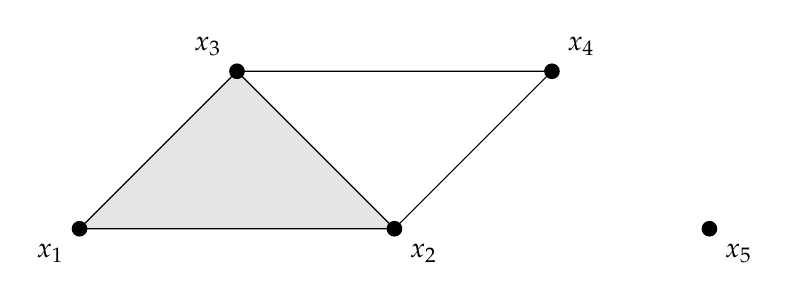
\begin{tikzpicture}

\draw[fill=gray!20] (0,0) -- (2,2) -- (4,0)-- (0,0);
\draw (2,2) -- (6,2) -- (4,0);

\node[circle, fill=black, inner sep=2pt, label=below left:$x_1 $] (a) at (0,0) {};
\node[circle, fill=black, inner sep=2pt, label=above left:$x_3 $] (b) at (2,2) {};
\node[circle, fill=black, inner sep=2pt, label=below right:$x_2 $] (c) at (4,0) {};
\node[circle, fill=black, inner sep=2pt, label=above right:$x_4 $] (c) at (6,2) {};
\node[circle, fill=black, inner sep=2pt, label=below right:$x_5 $] (c) at (8,0) {};




\end{tikzpicture} \end{center}

Note that $\Delta$ is completely specified by its facets. \end{example} 

~~~Let $\Delta$ be a simplicial complex on $\{x_{1},x_{2},\dots,x_{n}\}$.
For $i\in\mathbb{Z}$, let $F_{i}(\Delta)$ be the set of $i$-dimensional
faces of $\Delta$, and let $K^{F_{i}(\Delta)}$ be a $K$-vector
space whose basis elements $e_{\sigma}$ correspond to the $i$-faces
$\sigma\in F_{i}(\Delta)$. The (\textbf{augmented }or \textbf{reduced})
\textbf{chain complex of} $\Delta$ \textbf{over $K$ }is the complex 

\begin{center}\begin{tikzcd} \widetilde{\mathcal{C}}_{\bullet } (\Delta ; K): &  0  & K^{F_{-1} (\Delta ) } \arrow[l] & \cdots \arrow[l, "\partial _{0} ", swap]  & K^{F_{i-1} (\Delta ) } \arrow[l, "\partial _{i-1} ", swap] &   K^{F_{i} (\Delta ) } \arrow[l, "\partial _{i} ", swap] & \cdots  \arrow[l, "\partial _{i+1} ", swap] &  K^{F_{n-1} (\Delta ) } \arrow[l, "\partial _{n-1} ", swap] & 0 \arrow[l] \end{tikzcd}\end{center} 

where for an $i$-face $\sigma$, 
\[
\partial_{i}(e_{\sigma})=\sum_{j\in\sigma}\text{sign}(j,\sigma)e_{\sigma\backslash\{j\}}.
\]
Here $\text{sign}(j,\sigma)=(-1)^{r-1}$ if $j$ is the $r$th element
of the set $\sigma$, written in increasing order (since we are working
over a characteristic $2$ filed though, we can drop the sign all
together and simply write $\partial_{i}(e_{\sigma})=\sum_{j\in\sigma}e_{\sigma\backslash\{j\}}$).
For $i\in\mathbb{Z}$, we define the $i$\textbf{th reduced homology
}of $\Delta$ over $K$ as 
\[
\widetilde{H}_{i}(\Delta,K):=\text{Ker}(\partial_{i})/\text{Im}(\partial_{i+1}).
\]

In particular, $\widetilde{H}_{n-1}(\Delta;K)=\text{Ker}(\partial_{n-1})$
and $\widetilde{H}_{i}(\Delta;K)=0$ for $i<0$ or $n-1<i$, unless
$\Delta=\{\emptyset\}$, in which case $\widetilde{H}_{-1}(\Delta;K)\cong K$
and $\widetilde{H}_{i}(\Delta;K)=0$ for $i\geq0$. The dimension
of $\widetilde{H}_{0}(\Delta;K)$ as a $K$-vector space is one less
than the number of connected components of $\Delta$. Elements of
$\text{Ker}(\partial_{i})$ are called $i$\textbf{-cycles }and elements
of $\text{Im}(\partial_{i+1})$ are called $i$\textbf{-boundaries}. 

\begin{example}\label{example} For $\Delta$ as in Example~(\ref{examplesimplicialcomplex}),
we have 
\begin{align*}
F_{2}(\Delta) & =\{\{1,2,3\}\}\\
F_{1}(\Delta) & =\{\{1,2\},\{1,3\},\{2,3\},\{2,4\},\{3,4\}\}\\
F_{0}(\Delta) & =\{\{1\},\{2\},\{3\},\{4\},\{5\}\}\\
F_{-1}(\Delta) & =\{\emptyset\}
\end{align*}

Choosing bases for the $K^{F_{i}(\Delta)}$ as suggested by the ordering
of the faces listed above, the chain complex for $\Delta$ becomes
\begin{center}\begin{tikzcd}[ampersand replacement=\&] 

0 \& K \arrow[l] \& \& \&  K^5 \arrow[swap]{lll}{\begin{pmatrix} 1 & 1 & 1 & 1 & 1 \end{pmatrix} } \& \& \& \&   K^5 \arrow[swap]{llll}{ \begin{pmatrix} 1 & 1 & 0 & 0 & 0 \\ 1 & 0 & 1 & 1 & 0 \\ 0 & 1 & 1 & 0 & 1  \\ 0 & 0 & 0 & 1 & 1 \\ 0 & 0 & 0 & 0 & 0 \end{pmatrix} } \& \& K \arrow[swap]{ll}{\begin{pmatrix} 1 \\ 1 \\ 1 \\ 0 \\ 0 \end{pmatrix} } \& 0 \arrow[l]



\end{tikzcd}\end{center}

For example, $\partial_{2}(e_{\{1,2,3\}})=e_{\{2,3\}}+e_{\{1,3\}}+e_{\{1,2\}}$,
which we identify with the vector $(1,1,1,0,0)$. The mapping $\partial_{1}$
has rank $3$, so $\widetilde{H}_{0}(\Delta;K)\cong\widetilde{H}_{1}(\Delta;K)\cong K$
and the other homology groups are $0$. Geometrically, $\widetilde{H}_{0}(\Delta;K)$
is nontrivial since $\Delta$ is disconnected and $\widetilde{H}_{1}(\Delta;K)$
is nontrivial since $\Delta$ contains a triangle which is not the
boundary of an element of $\Delta$. \end{example} 

~~~We now introduce some notation. There is a bijection between
the set of subsets of $\{x_{1},x_{2},\dots,x_{n}\}$ and the set of
squarefree monomials in the variables $x_{1},x_{2},\dots,x_{n}$.
Namely, if $m$ is a squarefree monomial, then the corresonding subset
of $\{x_{1},x_{2},\dots,x_{n}\}$ is $\text{supp}(m)$. It is easy
see that if $m$ and $m'$ are squarefree monomials, then $m$ divides
$m'$ if and only if $\text{supp}(m)\subseteq\text{supp}(m')$. For
now on, we will abuse notation without comment by writing squarefree
monomials in place of subsets of $\{x_{1},x_{2},\dots,x_{n}\}$. The
reason that we make this change of notation is because, under this
correspondence, the boundary map defined on simplices precisely matches
the differential $d$ acting on monomials. Here's how we think of
the squarefree monomials in $x,y,z$ sit on the $2$-simplex:

\begin{center}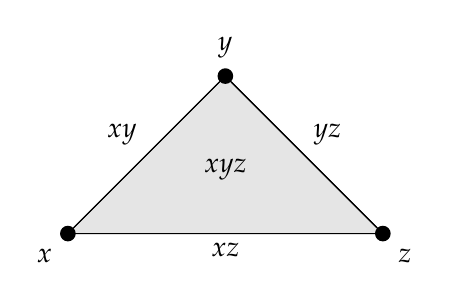
\begin{tikzpicture}

\draw[fill=gray!20] (0,0) -- (2,2) -- (4,0)-- (0,0);

\node[circle, fill=black, inner sep=2pt, label=below left:$x $] (a) at (0,0) {};
\node[circle, fill=black, inner sep=2pt, label=above :$y $] (b) at (2,2) {};
\node[circle, fill=black, inner sep=2pt, label=below right:$z $] (c) at (4,0) {};


\draw[] (a) -- (b) node [midway, above left] {$ xy $};
\draw[] (b) -- (c) node [midway, above right] {$ yz $};
\draw[] (c) -- (a) node [midway, below ] {$ xz $};

\node[label=below:$xyz$] (f) at (2,1.2) {};




\end{tikzpicture} \end{center} 

With this in mind, let's restate the definition of a simlicial complex
using this language: 

\begin{defn}\label{defn} An (abstract) \textbf{simplicial complex
$\Delta$ }on the set $\{x_{1},x_{2},\dots,x_{n}\}$ is a set of squarefree
monomials in the variables $x_{1},x_{2},\dots,x_{n}$ such that
\begin{enumerate}
\item $x_{\lambda}\in\Delta$ for all $\lambda=1,2,\dots,n$.
\item If $m$ is a squarefree monomial in $\Delta$, and $m'$ is a squarefree
monomial that divides $m$, then $m'$ is in $\Delta$. 
\end{enumerate}
\end{defn}

\subsection{Simplicial Join, Closure, Stars, and Links}

\subsubsection{Simplicial Join}

\begin{defn}\label{defn} Let $S_{x}$ be a set of squarefree monomials
in $x_{1},\dots,x_{m}$ and let $S_{y}$ be a set of squarefree monomials
in $y_{1},\dots,y_{n}$. Then the join of $S_{x}$ and $S_{y}$, denoted
$S_{x}\star S_{y}$, is the set of squarefree monomials in $x_{1},\dots,x_{m},y_{1},\dots,y_{n}$
of the form $m_{x}m_{y}$, where $m_{x}$ is in $S_{x}$ and $m_{y}$
is in $S_{y}$. \end{defn}

\begin{rem}\label{rem} Let $\Delta$ be a simplicial complex on $\{x_{1},\dots,x_{m}\}$
and $\Delta'$ be a simplicial complexes on $\{y_{1},\dots,y_{n}\}$.
Then it's easy to check that $\Delta\star\Delta'$ is a simplicial
complex on $\{x_{1},\dots,x_{m},y_{1},\dots,y_{n}\}$. Note that $1$
is considered a monomial in both $\Delta$ and $\Delta'$. In particular,
$x_{\lambda}\cdot1=x_{\lambda}$ and $y_{\mu}\cdot1=y_{\mu}$ are
in $\Delta\star\Delta'$. \end{rem}

\subsubsection{Closure, Stars, and Links}

~~~Let $m_{1}$ and $m_{2}$ be monomials in $S$. We write $m_{1}\perp m_{2}$
if $\text{supp}(m_{1})\cap\text{supp}(m_{2})=\emptyset$.

\begin{defn}\label{defn} Let $\Delta$ be a simplicial complex on
$\{x_{1},\dots,x_{n}\}$, and let $m$ be a squarefree monomial in
$\Delta$. 
\begin{enumerate}
\item The \textbf{star }of $m$, denoted $\text{St}(m)$, is the set of
all squarefree monomials $m'$ in $\Delta$ such that $m$ divides
$m'$. 
\item The \textbf{closure }of $m$, denoted $\text{Cl}(m)$, is the smallest
subcomplex of $\Delta$ which contains $\text{St}(m)$.
\item The \textbf{link }of $m$, denoted\textbf{ $\text{Lk}(m)$, }is the
subcomplex of $\Delta$ which consists of the squarefree monomials
$m'$ in $\Delta$ such that $m\perp m'$ and $mm'$ is in $\Delta$. 
\end{enumerate}
\end{defn}

\begin{rem}\label{rem} Every element in $\text{St}(m)$ can be written
as $m'm$ where $m'$ is a squarefree monomial in $S$ such that $m'\perp m$
and $m'm\in\Delta$. Similarly, every element in $\text{Cl}(m)$ can
be written as $\frac{m'm}{m''}$ where $m'$ and $m''$ are squarefree
monomials in $S$ such that $m'\perp m$, $m'm\in\Delta$, and $m''\mid m'm.$
When we write ``let $\frac{m'm}{m''}$ be an element in $\text{Cl}(m)$,
it is understood that $m'$ and $m''$ are squarefree monomials in
$S$ such that $m'\perp m$, $m'm\in\Delta$, and $m''\mid m'm.$
\end{rem}

\begin{example}\label{example} Let $\Delta$ be the simplical complex
as in Example~(\ref{examplesimplicialcomplex}). Then 
\begin{align*}
\text{Lk}(x_{1}x_{3})_{\text{max}} & =\{x_{2}\} & \text{Cl}(x_{1}x_{3})_{\text{max}} & =\{x_{1}x_{2}x_{3}\} & \text{St}(x_{1}x_{3}) & =\{x_{1}x_{2}x_{3},x_{1}x_{3}\}\\
\text{Lk}(x_{1})_{\text{max}} & =\{x_{2}x_{3}\} & \text{Cl}(x_{1})_{\text{max}} & =\{x_{1}x_{2}x_{3}\} & \text{St}(x_{1}) & =\{x_{1}x_{2}x_{3},x_{1}x_{3},x_{1}x_{2},x_{1}\}\\
\text{Lk}(x_{2})_{\text{max}} & =\{x_{1}x_{3},x_{4}\} & \text{Cl}(x_{2})_{\text{max}} & =\{x_{1}x_{2}x_{3},x_{2}x_{4}\} & \text{St}(x_{2}) & =\{x_{1}x_{2}x_{3},x_{2}x_{4},x_{2}x_{3},x_{1}x_{2},x_{2}\}\\
\text{Lk}(x_{4})_{\text{max}} & =\{x_{2},x_{3}\} & \text{Cl}(x_{4})_{\text{max}} & =\{x_{3}x_{4},x_{2}x_{4}\} & \text{St}(x_{4}) & =\{x_{3}x_{4},x_{2}x_{4},x_{4}\}\\
\text{Lk}(x_{5})_{\text{max}} & =\emptyset & \text{Cl}(x_{5})_{\text{max}} & =\{x_{5}\} & \text{St}(x_{5}) & =\{x_{5}\}
\end{align*}

where the ``max'' subscript denotes the subset of facets. \end{example}

\begin{prop}\label{prop} Let $\Delta$ be a simplicial complex on
$\{x_{1},\dots,x_{n}\}$. Then
\begin{enumerate}
\item $\text{St}(x_{\lambda})\cap\text{St}(x_{\mu})=\text{St}(x_{\lambda}x_{\mu}).$
More generally, we have 
\begin{equation}
\text{St}(m)=\bigcap_{x_{\lambda}\in\text{supp}(m)}\text{St}(x_{\lambda}).\label{eq:intersectionstar}
\end{equation}
\item $\text{Cl}(x_{\lambda})=\text{St}(x_{\lambda})\cup\text{Lk}(x_{\lambda})$.
\end{enumerate}
\end{prop}

\begin{proof} \hfill
\begin{enumerate}
\item A squarefree monomial $m$ belongs to $\text{St}(x_{\lambda})\cap\text{St}(x_{\mu})$
if and only if $x_{\lambda}\mid m$ and $x_{\mu}\mid m$ if and only
if $x_{\lambda}x_{\mu}\mid m$ if and only if $m$ belongs to $\text{St}(x_{\lambda}x_{\mu})$.
An easy induction argument gives us (\ref{eq:intersectionstar}).
\item Let $\frac{x_{\lambda}m}{m'}$ be an element in $\text{Cl}(x_{\lambda})$.
If $m'\mid m$, then $x_{\lambda}\cdot\frac{m}{m'}\in\text{St}(x_{\lambda})$.
If $m'\not\mid m$, then $m'=x_{\lambda}$ and thus $\frac{x_{\lambda}m}{m'}=m\in\text{Lk}(x_{\lambda})$.
Therefore, $\text{Cl}(x_{\lambda})\subset\text{St}(x_{\lambda})\cup\text{Lk}(x_{\lambda})$.
For the reverse inclusion, we already know that $\text{St}(x_{\lambda})\subset\text{Cl}(x_{\lambda})$,
so we just need to show that $\text{Lk}(x_{\lambda})\subset\text{Cl}(x_{\lambda})$.
Let $m\in\text{Lk}(x_{\lambda})$. This means that $x_{\lambda}\perp m$
and $x_{\lambda}m\in\Delta$. Then $x_{\lambda}m\in\text{St}(x_{\lambda})$
and so $m=\frac{x_{\lambda}m}{x_{\lambda}}\in\text{Cl}(x_{\lambda})$. 
\end{enumerate}
\end{proof}

\subsection{Squarefree Monomials and Stanley-Reisner Ring}

\subsubsection{Stanley-Reisner Ring}

~~~Let $\Delta$ be a simplicial complex on $\{x_{1},x_{2},\dots,x_{n}\}$.
We denote by $I_{\Delta}$ to be the ideal of nonfaces of $\Delta$,
i.e. $I_{\Delta}$ is generated by the squarefree monomials $m$ in
$S$ which are not in $\Delta$. We define the \textbf{Stanley-Reisner
ring }$K[\Delta]$ of the simplicial complex $\Delta$ to be the $K$-algebra
$K[\Delta]:=S/I_{\Delta}$. We will also denote by $I_{\Delta}^{\text{sq}}$
to mean $I_{\Delta}^{\text{sq}}:=\langle I_{\Delta},x_{1}^{2},\dots,x_{n}^{2}\rangle$. 

~~~Conversely, if $I$ is a squarefree monomial ideal in $S$.
Then we denote by $\Delta_{I}$ the simplicial complex on $\{x_{1},x_{2},\dots,x_{n}\}$
whose ideal of nonfaces is $I$, i.e. $\Delta_{I}$ consists of all
squarefree monomials which do not belong to $I$. 

\begin{example}\label{example} Consider $S=K[x_{1},x_{2},x_{3},x_{4},x_{5}]$
and $I_{\Delta}=\langle x_{1}x_{4},x_{1}x_{5},x_{2}x_{5},x_{2}x_{3}x_{4},x_{3}x_{5},x_{4}x_{5}\rangle$.
Then $S/I_{\Delta}$ is the Stanley-Reisner ring of the simplex $\Delta$
given in Example~(\ref{examplesimplicialcomplex}). From the correspondence
between squarefree monomials and simplices, we obtain an isomorphism
of chain complexes over $K$ from $\widetilde{C}_{\bullet}(\Delta;K)$
to $\mathbf{A}_{\bullet}(S_{I_{\Delta}^{\text{sq}}})$. Let's write
down each homogeneous piece side by side:
\begin{align*}
K^{F_{2}(\Delta)} & =Ke_{\{1,2,3\}} & (S_{I_{\Delta}^{\text{sq}}})_{_{3}} & =Kx_{1}x_{2}x_{3}\\
K^{F_{1}(\Delta)} & =Ke_{\{1,3\}}+Ke_{\{1,2\}}+Ke_{\{2,3\}}+Ke_{\{2,4\}}+Ke_{\{3,4\}} & (S_{I_{\Delta}^{\text{sq}}})_{_{2}} & =Kx_{1}x_{3}+Kx_{1}x_{2}+Kx_{2}x_{3}+Kx_{2}x_{4}+Kx_{3}x_{4}\\
K^{F_{0}(\Delta)} & =Ke_{\{1\}}+Ke_{\{2\}}+Ke_{\{3\}}+Ke_{\{4\}}+Ke_{\{5\}} & (S_{I_{\Delta}^{\text{sq}}})_{_{1}} & =Kx_{1}+Kx_{2}+Kx_{3}+Kx_{4}+Kx_{5}\\
F_{-1}(\Delta) & =K_{e_{\emptyset}} & (S_{I_{\Delta}^{\text{sq}}})_{_{0}} & =K
\end{align*}
As mentioned above, the way the differential acts on squarefree monomials
precisely matches the way the boundary map acts on the corresponding
simplices. It follows that $H_{i}(S_{I_{\Delta}^{\text{sq}}})\cong\widetilde{H}_{i-1}(\Delta;K)$.
In partciular, $H_{2}(S_{I_{\Delta}^{\text{sq}}})=\left[d(x_{2}x_{3}x_{4})\right]K$
and $H_{1}(S_{I_{\Delta}^{\text{sq}}})=\left[d(x_{2}x_{5})\right]K.$
\end{example}

\begin{rem}\label{rem} In fact, it turns out that $H_{i}(S_{I_{\Delta}})\cong H_{i}(S_{I_{\Delta}^{\text{sq}}})$.
\end{rem}

\begin{prop}\label{prop} Let $I$ be a squarefree monomial ideal
and let $\Delta_{I}$ be its corresponding simplicial complex. Let
$m$ be a squarefree monomial which is not in $I$. Then $I:m$ is
the squarefree monomial ideal whose corresponding simplicial complex
is $\Delta_{I:m}=\text{Cl}(m)$. \end{prop}

\begin{proof} Let $G=\{m_{1},\dots,m_{r}\}$ be the unique reduced
basis of $I$. We obtain the unique reduced basis of $I:m$ as follows:
if $m_{\lambda}\in G$ such that $m_{\lambda}=m\widetilde{m}_{\lambda}$
where $\widetilde{m}_{\lambda}$ is a squarefree monomial in $S$
such that $\widetilde{m}_{\lambda}\perp m$, then we replace $m_{\lambda}$
with $\widetilde{m}_{\lambda}$. We do this for each such $m_{\lambda}$
in $G$ to get a new set $\widetilde{G}$. Then $\widetilde{G}$ is
the unique reduced basis of $I:m$. Each monomial in $\widetilde{G}$
is clearly squarefree, and thus $I:m$ is squarefree. 

~~~ Let $m'\in\Delta_{I:m}$. This means that $mm'\notin I$. We
want to show that $m'\in\text{Cl}(m)$. Since $I$ is squarefree,
we may assume that $\text{supp}(m')\cap\text{supp}(m)=\emptyset$.
But then this implies that $m'\in\text{Lk}(m)\subset\text{Cl}(m)$,
since $mm'\notin I$ is equivalent to saying $mm'\in\Delta_{I}$. 

\end{proof}

\begin{proof} Let $\frac{m'm}{m''}\in\text{Cl}(m)$. If $m'\perp m$,
then $m'\in\text{Lk}(m)$, since we must have $m'm\in\Delta_{I}$.
\end{proof}

Let $m'$ be a squarefree monomial in $\Delta_{I:m}$. This means
that $mm'$ does not belong to $I$. 

\begin{prop}\label{prop} Let $I$ be a squarefree monomial ideal
and let $m$ be a . Then $I:m$ is the squarefree monomial ideal whose
corresponding simplicial complex is $\Delta_{I:m}=\text{Cl}(m)$.
\end{prop}

\begin{prop}\label{prop} Let $I$ be a squarefree monomial ideal
and let $\Delta_{I}$ be its corresponding simplicial complex. Then
$I:x_{\lambda}^{2}=I:x_{\lambda}$. Moreover, $I:x_{\lambda}$ is
the squarefree monomial ideal whose corresponding simplicial complex
is $\Delta_{I:x_{\lambda}}=\text{Cl}(x_{\lambda})$. \end{prop}

\begin{proof} We have $I:x_{\lambda}^{2}=I:x_{\lambda}$ since $I$
is a squarefree monomial ideal: let . An element 

Let $m$ be a squarefree monomial in $\Delta_{I:x_{\lambda}}$. This
means that $x_{\lambda}m$ does not belong to $I$. We may assume
that $m\perp x_{\lambda}$ (otherwise, we consider $m/x_{\lambda}$).
Then $m\in\text{Cl}(x_{\lambda})$ since $m=\frac{x_{\lambda}m}{x_{\lambda}}$
where $x_{\lambda}m\in\text{St}(x_{\lambda})$ and $x_{\lambda}\mid x_{\lambda}m$.
\end{proof}

\section{Generalizing from Characteristic $2$ to any Characteristic}

~~~In this section, we want to show how to generalize all of our
previous constructions by replacing the base field $\mathbb{F}_{2}$
with an arbitrary field $K$ whose characteristic is not necessarily
equal to $2$. 

\subsection{Non-Commutative $G$-Algebras}

~~~Let $K\langle x_{1},\dots,x_{n}\rangle$ be the free associative
$K$-algebra, generated by $\{x_{1},\dots,x_{n}\}$ over $K$. A $K$-basis
of $K\langle x_{1},\dots,x_{n}\rangle$ consists of \textbf{words
$x_{i_{1}}^{\alpha_{1}}x_{i_{2}}^{\alpha_{2}}\cdots x_{i_{r}}^{\alpha_{r}}$},
where $1\leq i_{1},i_{2},\dots,i_{r}\leq n$ with $r\geq0$ and $\alpha_{i}\ge0$.
The elements of the form \textbf{$x_{i_{1}}^{\alpha_{1}}x_{i_{2}}^{\alpha_{2}}\cdots x_{i_{r}}^{\alpha_{r}}$},
with ordered indices $1\leq i_{1}<i_{2}<\cdots<i_{r}\leq n$, are
often called \textbf{standard words }and form a subset of the set
of all words. The main difference between standard words and monomials
is that the ordering matters! For instance, $xy^{2}$ is a standard
word in $K\langle x,y\rangle$ but $y^{2}x$ is not a standard work
in $K\langle x,y\rangle$, even though we consider both $xy^{2}$
and $y^{2}x$ to be monomials in $K[x,y]$. In this case, we can simply
write a standard words as $x_{1}^{\alpha_{1}}x_{2}^{\alpha_{2}}\cdots x_{n}^{\alpha_{n}}$.

~~~We can simplify the notation for standard words as follows:
Let $\alpha=(\alpha_{1},\dots,\alpha_{n})$ be an $n$-tuple of nonnegative
integers. Then we set
\[
x^{\alpha}:=x_{1}^{\alpha_{1}}x_{2}^{\alpha_{2}}\cdots x_{n}^{\alpha_{n}}.
\]

Note that $x^{\alpha}=1$ when $\alpha=(0,\dots,0)$. We also denote
$|\alpha|:=\alpha_{1}+\alpha_{2}+\cdots+\alpha_{n}$ and call this
the \textbf{degree }of $x^{\alpha}$. A \textbf{standard polynomial
}$f$ in $K\langle x_{1},\dots,x_{n}\rangle$ with coefficients in
a field $K$ is a finite linear combination of standard words. We
will write a standard polynomial $f$ in the form 
\[
f=\sum_{\alpha}a_{\alpha}x^{\alpha},\quad a_{\alpha}\in K,
\]
where the sum is over a finite number of $n$-tuples $\alpha=(\alpha_{1},\dots,\alpha_{n})$.
If $a_{\alpha}\neq0$, then we call $a_{\alpha}x^{\alpha}$ a term
of $f$ and $x^{\alpha}$ a standard word of $f$. We say that $f$
is \textbf{homogeneous of degree $i$ }if all the standard words of
$f$ have degree $i$. 

\subsection{Anticommutative Polynomial Rings}

~~~Every finitely presented associative $K$-algebra $A$ is isomorphic
to $K\langle x_{1},\dots,x_{n}\rangle/I$ for some $n\in\mathbb{N}$
and some two-sided ideal $I$ in $K\langle x_{1},\dots,x_{n}\rangle$.
For our purposes we will be interested in the following finitely presented
$K$-algebra, which we denote by $T$:
\[
T:=K\langle x_{1},\dots,x_{n}\rangle/\langle x_{j}x_{k}+x_{k}x_{j}\mid1\leq j<k\leq n\rangle.
\]
Here, $\langle x_{j}x_{k}+x_{k}x_{j}\mid1\leq j<k\leq n\rangle$ is
the two sided ideal in $K\langle x_{1},\dots,x_{n}\rangle$ generated
by $\{x_{j}x_{k}+x_{k}x_{j}\mid1\leq j<k\leq n\}$. We often call
$T$ the \textbf{anticommutive polynomial ring}. Note that a ring
$R$ is assumed to be commutative, so we must be careful using this
terminology. However, we believe our terminology is justified since
$T$ behaves very much like the \emph{polynomial ring} $S$. The main
difference between $T$ and $S$ is that we have the anticommutative
relations for distinct variables in $T$: 
\[
x_{j}x_{k}=-x_{k}x_{j}\text{ whenever }j\neq k.
\]

~~~On the other hand, there are a plethora of similarities. For
instance, just like how the polynomial ring $S$ is a graded $K$-algebra,
where the homogeneous component $S_{i}$ is the $K$-vector space
of all homogeneous polynomials $f\in S$ of degree $i$, the anticommutative
polynomial ring $T$ is a graded $K$-algebra, where the homogeneous
component $T_{i}$ is the $K$-vector space of all homogeneous standard
polynomials $f\in S$ of degree $i$. By a graded $K$-algebra, we
mean there is a direct sum $T=\bigoplus_{i\geq0}T_{i}$ where $T_{i}T_{j}\subseteq T_{i+j}$,
$T_{j}T_{i}\subseteq T_{i+j}$, and $T_{0}=K$.

\begin{example}\label{example} Consider the anticommutative polynomial
ring $T=K\langle x,y,z\rangle/\langle xy+yx,xz+zx,yz+zy\rangle$ and
the polynomial ring $S$. In $T$, we have the anticommuative relations
$xy=-yx$, $xz=-zx$, and $yz=-zy$. In $S$, we have the commutative
relations $xy=yx$, $xz=zx$, and $yz=zy$. Let's write the first
few homogeneous terms of $T$ and $S$:
\begin{align*}
T_{0} & =K & S_{0} & =K\\
T_{1} & =Kx+Ky & S_{1} & =Kx+Ky\\
T_{2} & =Kx^{2}+Kxy+Ky^{2} & S_{2} & =Kx^{2}+Kyx+Ky^{2}\\
T_{3} & =Kx^{3}+Kx^{2}y+Kxy^{2}+Ky^{3} & S_{3} & =Kx^{3}+Kyx^{2}+Kxy^{2}+Ky^{3}\\
 & \vdots &  & \vdots
\end{align*}

\end{example}

\subsubsection{Differential}

~~~We want to construct a \textbf{differential map $d$ for $T$
}in analogy to the differential map for $S$. We construct the map
as follows: We first set $d(x_{j})=1$ for all $x_{j}$ where $1\leq j\leq n$.
Next, we use the Leibniz law (\ref{eq:leibniz1}) to extend this map
to standard words $x_{i_{1}}^{\alpha_{1}}x_{i_{2}}^{\alpha_{2}}\cdots x_{i_{r}}^{\alpha_{r}}$.
Now that we've defined $d$ on the set of standard words, we turn
it into a $K$-linear map by extending it linearly to all of $T$.
We also have $d^{2}=0$. Then 

\begin{example}\label{example} Let's do some computations in the
anticommutative polynomial ring $T$ in three variables $x,y,z$.
Our goal is to calculate $d(x^{3}+xyz+2yz^{2})$. First let's calculate
$d(x^{3})$: 

\begin{align*}
d(x^{3}) & =d(x)x^{2}-xd(x^{2})\\
 & =x^{2}-x(d(x)x-xd(x))\\
 & =x^{2}.
\end{align*}

Next, let's calculate $d(xyz)$:
\begin{align*}
d(xyz) & =d(x)yz-xd(yz)\\
 & =yz-x(d(y)z-yd(z))\\
 & =yz-x(z-y)\\
 & =yz-xz+xy
\end{align*}

Next, let's calculate $d(2yz^{2})$
\begin{align*}
d(2yz^{2}) & =2d(yz^{2})\\
 & =2(d(y)z^{2}-yd(z^{2}))\\
 & =2z^{2}.
\end{align*}

Combining everything together, we have 
\begin{align*}
d(x^{3}+xyz+2yz^{2}) & =d(x^{3})+d(xyz)+d(2yz^{2})\\
 & =x^{2}+yz-xz+xy+2z^{2}.
\end{align*}
\end{example} 

~~~It is clear from the way we constructed $d$ that it gives $T$
the structure of a differential graded algebra over $K$. 

\part{Homological Constructions over a Ring of Characteristic $2$}

~~~Throughout this part of the article, let $R$ be a ring of characteristic
$2$ and let $a_{1},\dots,a_{n}\in R$ be nonzero elements in $R$.
We let $S$ denote the \textbf{polynomial ring over} $R$. That is,

\[
S:=R[x_{1},\dots,x_{n}].
\]
Our aim in this part of article is to generalize the differential
graded algebra constructions done in Part II by replacing the base
field $\mathbb{F}_{2}$ with the ring $R$. 

\section{Constructing the Differential Graded $R$-algebra $(S,a_{1},\dots,a_{n})$}

\subsection{Defining the Differential}

~~~The polynomial ring $S$ over $R$ is a graded $R$-algebra,
where the homogeneous component $S_{i}$ is the free $R$-module generated
by the monomials of degree $i$. We want to construct a map $d:S\to S$
which gives $S$ the structure of a differential graded $R$-algebra.
Informally, this map will be $d:=\sum_{\lambda=1}^{n}a_{\lambda}\partial_{x_{\lambda}}$:
If $f$ is a homogeneous polynomial in $S$, expressed in the monomial
basis as
\[
f=\sum_{\lambda=1}^{r}b_{\lambda}x_{1}^{\alpha_{1\lambda}}\cdots x_{\mu}^{\alpha_{\mu\lambda}}\cdots x_{n}^{\alpha_{n\lambda}},
\]
 where $b_{\lambda}\in R$ and $\alpha_{\mu\lambda}\in\mathbb{Z}_{\geq0}$
for all $\lambda=1,\dots,r$ and $\mu=1,\dots,n$. Then
\[
d(f)=\sum_{\substack{1\leq\mu\leq n\\
1\leq\lambda\leq r
}
}\alpha_{\mu\lambda}a_{\mu}b_{\lambda}x_{1}^{\alpha_{1\lambda}}\cdots x_{\mu}^{\alpha_{\mu\lambda}-1}\cdots x_{n}^{\alpha_{n\lambda}},
\]
where $\alpha_{\mu\lambda}a_{\mu}b_{\lambda}x_{1}^{\alpha_{1\lambda}}\cdots x_{\mu}^{\alpha_{\mu\lambda}-1}\cdots x_{n}^{\alpha_{n\lambda}}=0$
if $\alpha_{\mu\lambda}$ is even (remember, we are working in characteristic
$2$).

~~~We want to construct this map in a more formal way. We do this
in the following way: First we define $d$ on $R$ as $d(r)=0$ for
all $r$ in $R$. Now, we define $d$ on the monomials in $S$ by
induction on the degree of the monomial.
\begin{itemize}
\item \textbf{Base Case: }We define $d(x_{\lambda}):=a_{\lambda}$ for all
$1\leq\lambda\leq n$. 
\item \textbf{Induction}: Assume that $d$ is defined on all monomials of
degree $i\geq1$. Let $m$ be a monomial of degree $i+1$. Then we
can decompose $m$ as $m=x_{\lambda}m_{\lambda}$ for some $1\leq\lambda\leq n$
where $m_{\lambda}$ is a monomial of degree $i$. Using the decomposition
together with the induction step, we define
\begin{align*}
d(m) & :=d(x_{\lambda}m_{\lambda})\\
 & :=d(x_{\lambda})m_{\lambda}+x_{\lambda}d(m_{\lambda})\\
 & =a_{\lambda}m_{\lambda}+x_{\lambda}d(m_{\lambda}).
\end{align*}
\end{itemize}
Observe that the induction step does not depend on the decomposition.
We can prove this again by induction on the degree of the monomial: 
\begin{itemize}
\item \textbf{Base Case: }If $m$ is a monomial of degree $2$, then we
can decompose $m$ in two wasy: as $m=x_{\lambda}x_{\mu}$ or $m=x_{\mu}x_{\lambda}$.
It is clear that $d$ is well-defined in this case. 
\item \textbf{Induction}: Assume that $d$ is well-defined on all monomials
of degree $i\geq1$. Let $m$ be a monomial of degree $i+1$ and let
$m=x_{\lambda}m_{\lambda}$ and $m=x_{\mu}m_{\mu}$ be two decompositions
of $m$. Then using the decomposition $m=x_{\lambda}m_{\lambda}$,
we have 
\begin{align*}
d(m) & =a_{\lambda}m_{\lambda}+x_{\lambda}d(m_{\lambda})\\
 & =a_{\lambda}m_{\lambda}+x_{\lambda}d(x_{\mu}m_{\mu\lambda})\\
 & =a_{\lambda}m_{\lambda}+x_{\lambda}a_{\mu}m_{\mu\lambda}+x_{\lambda}x_{\mu}d(m_{\mu\lambda})\\
 & =a_{\lambda}m_{\lambda}+x_{\lambda}a_{\mu}x_{\mu}^{-1}x_{\lambda}^{-1}m+x_{\lambda}x_{\mu}d(m_{\mu\lambda})\\
 & =a_{\lambda}m_{\lambda}+a_{\mu}x_{\mu}^{-1}m+x_{\lambda}x_{\mu}d(m_{\mu\lambda})\\
 & =a_{\lambda}m_{\lambda}+a_{\mu}m_{\mu}+x_{\lambda}x_{\mu}d(m_{\mu\lambda})
\end{align*}
where we used the fact that $m_{\mu\lambda}=x_{\mu}^{-1}x_{\lambda}^{-1}m$
and $m_{\mu}=x_{\mu}^{-1}m$. On other hand, using the decomposition
$m=x_{\mu}m_{\mu}$, a similar computation shows us that 
\[
d(m)=a_{\mu}m_{\mu}=a_{\lambda}m_{\lambda}+x_{\mu}x_{\lambda}d(m_{\lambda\mu}).
\]
Therefore, both decompositions lead to the same result. 
\end{itemize}
~~~Now that $d$ is defined on all monomials, we define $d$ on
all homogeneous polynomials $f$ of degree $i$, by extending $d$
$R$-linearly. Thus, if we express $f$ in terms of the monomial basis,
say $f=c_{1}m_{1}+\cdots+c_{k}m_{k}$, then 
\[
d(f):=c_{1}d(m_{1})+\cdots+c_{k}d(m_{k}).
\]

\subsection{Showing that the Differential Satisfies Leibniz Law}

~~~Given the way $d$ is defined, we see that $d:S\to S$ is a
graded $R$-linear map of degree $-1$. We now want to show that $d$
satisfies Leibniz law. To do this, we first show that it satisfies
Leibniz law for all pairs of monomials.

\begin{prop}\label{prop} Let $m_{1}$ and $m_{2}$ be monomials in
$S$. Then
\[
d(m_{1}m_{2})=d(m_{1})m_{2}+m_{1}d(m_{2}).
\]
\end{prop}

\begin{proof} We prove this by induction on the degree of $m_{1}m_{2}$.
For the base case, we have 
\[
d(x_{\lambda}x_{\mu})=d(x_{\lambda})x_{\mu}+x_{\lambda}d(x_{\mu})
\]
by definition. Now assume that the proposition is true for all monomials
$m_{1}$ and $m_{2}$ such that $\text{deg}(m_{1}m_{2})\leq i$. Let
$m_{1}$ and $m_{2}$ be two monomials such that $\text{deg}(m_{1}m_{2})=i+1$.
If $\text{deg}(m_{1})=0$ or $\text{deg}(m_{2})=0$, then the Leibniz
law is obviously satisfied. Therefore, we may assume that $\text{deg}(m_{1})>0$
and $\text{deg}(m_{2})>0$. Let $m_{1}=x_{\lambda}m$ be a decomposition
of $m_{1}$. Then $\text{deg}(mm_{2})\leq i$ and $d(x_{\lambda}m)\leq i$,
and so by induction, we have 
\begin{align*}
d(m_{1}m_{2}) & =d(x_{\lambda}mm_{2})\\
 & =d(x_{\lambda})mm_{2}+x_{\lambda}d(mm_{2})\\
 & =a_{\lambda}mm_{2}+x_{\lambda}\left(d(m)m_{2}+md(m_{2})\right)\\
 & =a_{\lambda}mm_{2}+x_{\lambda}d(m)m_{2}+x_{\lambda}md(m_{2})\\
 & =(d(x_{\lambda})m+x_{\lambda}d(m))m_{2}+x_{\lambda}md(m_{2})\\
 & =d(x_{\lambda}m)m_{2}+x_{\lambda}md(m_{2})\\
 & =d(m_{1})m_{2}+m_{1}d(m_{2}).
\end{align*}
\end{proof}

~~~Now we show that Leibniz law is satisfied for all pairs of homogeneous
polynomials.

\begin{prop}\label{prop} Let $f_{1}$ and $f_{2}$ be homogeneous
polynomials in $S$. Then 
\[
d(f_{1}f_{2})=d(f_{1})f_{2}+f_{2}d(f_{2})
\]
\end{prop}

\begin{proof} Write $f_{1}$ and $f_{2}$ in terms of the monomial
basis of $S$:
\[
f_{1}=\sum_{\lambda=1}^{r}b_{\lambda}m_{1\lambda}\qquad\text{and}\qquad f_{2}=\sum_{\mu=1}^{s}c_{\mu}m_{2\mu}
\]
 where $b_{\lambda},c_{\mu}\in R$ for all $1\leq\lambda\leq r$ and
$1\leq\mu\leq s$. Then
\begin{align*}
d\left(f_{1}f_{2}\right) & =d\left(\left(\sum_{\lambda=1}^{r}b_{\lambda}m_{1\lambda}\right)\left(\sum_{\mu=1}^{s}c_{\mu}m_{2\mu}\right)\right)\\
 & =d\left(\sum_{\lambda,\mu}b_{\lambda}c_{\mu}m_{1\lambda}m_{2\mu}\right)\\
 & =\sum_{\lambda,\mu}b_{\lambda}c_{\mu}d\left(m_{1\lambda}m_{2\mu}\right)\\
 & =\sum_{\lambda,\mu}b_{\lambda}c_{\mu}\left(d(m_{1\lambda})m_{2\mu}+m_{1\lambda}d(m_{2\mu})\right)\\
 & =\sum_{\lambda,\mu}b_{\lambda}c_{\mu}d(m_{1\lambda})m_{2\mu}+\sum_{\lambda,\mu}b_{\lambda}c_{\mu}m_{1\lambda}d(m_{2\mu})\\
 & =\left(\sum_{\lambda=1}^{r}b_{\lambda}d(m_{1\lambda})\right)\left(\sum_{\mu=1}^{s}c_{\mu}m_{2\mu}\right)+\left(\sum_{\lambda=1}^{r}b_{\lambda}m_{1\lambda}\right)\left(\sum_{\mu=1}^{s}c_{\mu}d(m_{2\mu})\right)\\
 & =d\left(\sum_{\lambda=1}^{r}b_{\lambda}m_{1\lambda}\right)\left(\sum_{\mu=1}^{s}c_{\mu}m_{2\mu}\right)+\left(\sum_{\lambda=1}^{r}b_{\lambda}m_{1\lambda}\right)d\left(\sum_{\mu=1}^{s}c_{\mu}m_{2\mu}\right)\\
 & =d(f_{1})f_{2}+f_{1}d(f_{2}).
\end{align*}
\end{proof}

\subsubsection{Showing that the Differential Satisfies $d^{2}=0$}

~~~With Leibniz law established, it is easy to show that $d^{2}=0$.
Indeed, to show that $d^{2}=0$, it suffices to show that $d^{2}(m)=0$
for all monomials in $S$. We prove this in the next proposition. 

\begin{prop}\label{prop} For all monomials $m$ in $S$, we have
$d^{2}(m)=0$. \end{prop}

\begin{proof} We prove this by induction on the degree of $m$. For
the base case, we have 
\[
d^{2}(x_{\lambda})=d(a_{\lambda})=0.
\]
Now assume that the proposition is true for all monomials of degree
$i>1$. Let $m$ be a monomial of degree $i+1$. Then we can write
$m=m_{1}m_{2}$ where $m_{1}$ and $m_{2}$ are monomials of degree
$\leq i$. Thus, $d^{2}(m_{1})=d^{2}(m_{2})=0$ by induction. Therefore
\begin{align*}
d^{2}(m) & =d^{2}(m_{1}m_{2})\\
 & =d(d(m_{1})m_{2}+m_{1}d(m_{2}))\\
 & =d(d(m_{1})m_{2})+d(m_{1}d(m_{2}))\\
 & =d^{2}(m_{1})m_{2}+d(m_{1})d(m_{2})+d(m_{1})d(m_{2})+m_{1}d^{2}(m_{2})\\
 & =d(m_{1})d(m_{2})+d(m_{1})d(m_{2})\\
 & =0.
\end{align*}
\end{proof}

\subsubsection{The Differential $d$ Gives $S$ the Structure of a Differential
Graded $R$-Algebra}

~~~We have shown that the differential $d$ gives $S$ the structure
of a differential graded $R$-algebra. We denote this differential
graded $R$-algebra as $(S,a_{1},\dots,a_{n})$ and denote its homology
as $H(S,a_{1},\dots,a_{n})$. 

\section{Constructing the Differential Graded $R$-algebra $(S/I,a_{1},\dots,a_{n})$}

~~~Throughout this section, we fix a homogeneous ideal $I$ in
$S$. Recall that $S/I$ is a graded $R$-algebra. If $I$ satisfies
an additional condition, we can give $S/I$ the structure of a differential
graded $R$-algebra where the differential $\overline{d}$ on $S/I$
is induced by the differential $d$ on $S$. We state this additional
requirement in the next definition.

\begin{defn}\label{defn} Let $I$ be a homogeneous ideal in $S$.
We say $I$ is $d$-\textbf{stable }if $d$ maps $I$ into $I$. \end{defn}

\begin{theorem}\label{theoremdstablediffgradalg} Suppose $I$ is
$d$-stable. Then the differential $d:S\to S$ induces a graded linear
map of degree $-1$, denoted $\overline{d}:S/I\to S/I$, where 
\[
\overline{d}(\overline{f})=\overline{d(f)}\text{ for all }f\in S.
\]

Moreover, $\overline{d}$ gives $S/I$ the structure of a differential
graded $R$-algebra. \end{theorem}

\begin{proof} Indeed, the map $\overline{d}$ is well-defined since
$d$ is $I$-stable. To see why, let $f+g$ and $f,$ where $g\in I$
and $f\in S$, be two different representatives of a class in $S/I$,
i.e. $\overline{f+g}=\overline{f}\in S/I$. Then 
\begin{align*}
\overline{d}\left(\overline{f+g}\right) & =\overline{d(f+g)}\\
 & =\overline{d(f)+d(g)}\\
 & =\overline{d(f)}\\
 & =\overline{d}(\overline{f}).
\end{align*}

where $\overline{d(f)+d(g)}=\overline{d(f)}$ since $d(g)\in I$.
Also, $\overline{d}$ is a graded linear map of degree $-1$ such
that $\overline{d}^{2}=0$ and such that $\overline{d}$ satisfies
Leibniz law since it inherits these properties from $d$. \end{proof}

\begin{rem}\label{rem} If the context is clear, we will just write
$d$ instead of $\overline{d}$. \end{rem}

~~~We will formally denote this differential graded $R$-algebra
as $(S/I,a_{1},\dots,a_{n})$ and denote its homology as $H(S/I,a_{1},\dots,a_{n})$.
The next proposition gives a necessary and sufficient condition for
a finitely generated ideal $I$ to be $d$-stable.

\begin{prop}\label{propcriteriondstable} Let $I$ be a homogeneous
ideal in $S$. Then $I$ is $d$-stable if and only if for some generating
set $F=\{f_{1},\dots,f_{r}\}$ of $I$, we have $d(f_{\lambda})\in I$
for all $\lambda=1,\dots,r$. \end{prop}

\begin{proof} One direction is trivial, so let's prove the other
direction. Let $F=\{f_{1},\dots,f_{r}\}$ be a generating set for
$I$ such that $d(f_{\lambda})\in I$ for all $\lambda=1,\dots,r$
and let $f\in I$. Since $\{f_{1},\dots,f_{r}\}$ generates $I$,
we can write $f=\sum_{\lambda=1}^{r}q_{\lambda}f_{\lambda}$ for some
$q_{1},\dots,q_{r}\in S$. Thus, by Leibniz law, we have
\begin{align*}
d(f) & =d\left(\sum_{\lambda=1}^{r}q_{\lambda}f_{\lambda}\right)\\
 & =\sum_{\lambda=1}^{r}d(q_{\lambda}f_{\lambda})\\
 & =\sum_{\lambda=1}^{r}(d(q_{\lambda})f_{\lambda}+q_{\lambda}d(f_{\lambda}))\in I.
\end{align*}
Thus, $I$ is $d$-stable. \end{proof} 

\subsubsection{Koszul Complex}

~~~Suppose $I$ is generated by $\left\{ x_{1}^{2},\dots,x_{n}^{2}\right\} $.
Then $S/I$ is a differential graded $R$-algebra by Proposition~(\ref{propcriteriondstable}).
This differential graded $R$-algebra is isomorphic to the Koszul
complex of $\varphi$, where $\varphi:S_{1}:=\bigoplus_{\lambda=1}^{n}Rx_{\lambda}\to R$
is the unique $R$-linear map such that $\varphi(x_{\lambda})=a_{\lambda}$
for all $\lambda=1,\dots,n$. We denote this Koszul complex as $\mathcal{K}(a_{1},\dots,a_{n})$. 

\begin{example}\label{example} Let $R=\mathbb{F}_{2}[x,y]/\langle xy\rangle$
and let $a_{1}=x$ and $a_{2}=y$. Then $S=R[u,v]$ has a differential
graded $R$-algebra structure with the differential $d$ where $d(u)=x$
and $d(v)=y$. Using graded lexicographical ordering on the monomials,
we can explicitly write $S$ as a chain complex over $R$ using matrices
as the linear maps:

\begin{center}\begin{tikzcd}[ampersand replacement=\&] \cdots  \arrow[r] \& R^4 \arrow{rrrr}{\begin{pmatrix} s & t & 0 & 0 \\ 0 & 0 & 0 & 0 \\ 0 & 0 & s & t \end{pmatrix}} \& \& \& \& R^3 \arrow{rrr}{\begin{pmatrix} 0 & t & 0 \\ 0 & s & 0 \end{pmatrix}}  \& \& \& R^2 \arrow{rr}{\begin{pmatrix} s & t \end{pmatrix}}  \& \& R \arrow[r] \& 0  \end{tikzcd}\end{center}

~~~Now let $I$ be the homogeneous ideal in $S$ generated by $\{x^{2},y^{2}\}$.
Then $S/I$ is just the Koszul complex $\mathcal{K}(a_{1},a_{2})$.
Using graded lexicographical ordering on the monomials, we can explicitly
write $S/I$ as a chain complex over $R$ using matrices as the linear
maps:

\begin{center}\begin{tikzcd}[ampersand replacement=\&] 0 \arrow[r] \& R \arrow{rr}{\begin{pmatrix} t \\ s \end{pmatrix}}   \& \& R^2 \arrow{rr}{\begin{pmatrix} s & t \end{pmatrix}}  \& \& R \arrow[r] \& 0  \end{tikzcd}\end{center}

\end{example}

\subsubsection{Blow up algebras}

\begin{defn}\label{defnblowup} Let $Q$ be an ideal in $R$. The
\textbf{blowup algebra of $Q$ in $R$ }is the $R$-algebra
\[
B_{Q}(R):=R+tQ+t^{2}Q^{2}+t^{3}Q^{3}+\cdots\cong R\oplus Q\oplus Q^{2}\oplus Q^{3}\oplus\cdots.
\]

The multiplication in $B_{Q}(A)$ is induced by the multiplication
$Q^{i}\times Q^{j}\to Q^{i+j}$. \end{defn}

\begin{prop}\label{propblowupofneotherianisnoetherian} Let $R$ be
a Noetherian ring and $Q\subset R$ an ideal. Then $B_{Q}(R)$ is
a Noetherian ring. \end{prop}

\begin{proof} Since $R$ is Noetherian, $Q$ is finitely generated,
say $Q=\langle a_{1},\dots,a_{n}\rangle$. Then the map $\varphi:R[x_{1},\dots,x_{n}]\to B_{Q}(R)$,
induced by $\varphi(x_{\lambda})=ta_{\lambda}$ for all $\lambda=1,\dots,n$,
is a surjective ring homomorphism from a Noetherian ring. Therefore
$B_{Q}(R)$ is a Noetherian ring. \end{proof}

\begin{example}\label{exampleblowupalgebra} Let $R=\mathbb{F}_{2}[x,y]/\langle y^{2}+x^{3}+x^{2}\rangle$
and let $\mathfrak{m}$ be the maximal ideal in $R$ generated by
$\{\overline{x},\overline{y}\}$. Then
\[
S=R[u,v]\cong\mathbb{F}_{2}[x,y,u,v]/\langle y^{2}+x^{3}+x^{2}\rangle
\]
has a differential graded $R$-algebra structure where the differential
$d$ is induced by $d(u)=\overline{x}$ and $d(v)=\overline{y}$.
There is a surjective homomorphism from $S$ to the blow up algebra
at $\mathfrak{m}$ given by
\[
\varphi:S:=\mathbb{F}_{2}[x,y,u,v]/\langle y^{2}+x^{3}+x^{2}\rangle\to B_{\mathfrak{m}}(R),
\]
where $\varphi$ is induced by $\varphi(u)=t\overline{x}$ and $v\mapsto t\overline{y}$.
Using Singular, we find that the kernel of $\varphi$ is an ideal
which is homogeneous in the variables $u,v,$ and is generated by
given by $\{f_{1},f_{2},f_{3}\}$, where 
\begin{align*}
f_{1} & =\overline{x}v+\overline{y}u\\
f_{2} & =\overline{x}u^{2}+u^{2}+v^{2}\\
f_{3} & =\overline{x}^{2}u+\overline{x}u+\overline{y}v
\end{align*}
Observe that $d(f_{1})=d(f_{2})=d(f_{3})\in\text{Ker}(\varphi)$.
It follows from Proposition~(\ref{propcriteriondstable}) that $\text{Ker}(\varphi)$
is $d$-stable. Therefore the blowup algebra $B_{\mathfrak{m}}(R)\cong S/\text{Ker}(\varphi)$
is a differential graded $R$-algebra by Theorem~(\ref{theoremdstablediffgradalg}).
\end{example}

~~~Example~(\ref{exampleblowupalgebra}) seems to imply that blow
up algebras are differential graded $R$-algebras. The next theorem
tells us that this is indeed true.

\begin{theorem}\label{theoremblowupalgaisdgalg} Let $Q$ be a finitely
generated ideal in $R$ with generating set $\{a_{1},\dots,a_{n}\}$.
Then the blow up algebra $B_{Q}(R)$ is a differential graded $R$-algebra.
\end{theorem}

\begin{proof} Let $\varphi:S:=R[x_{1},\dots,x_{n}]\to B_{Q}(R)$
be the unique graded $R$-algebra homomorphism such that $\varphi(x_{\lambda})=ta_{\lambda}$
for all $\lambda=1,\dots,n$. If we can show that $\text{Ker}(\varphi)$
is $d$-stable, then Theorem~(\ref{theoremdstablediffgradalg}) would
imply that $B_{Q}(R)$ is a differential graded $R$-algebra. So let's
show that $\text{Ker}(\varphi)$ is $d$-stable. 

~~~Let $f\in\text{Ker}(\varphi)$. We will show that $\varphi(d(f))=0$,
and hence $\text{Ker}(\varphi)$ is $d$-stable. Since $\text{Ker}(\varphi)$
is a homogeneous ideal, we may assume that $f$ is homogeneous, say
of degree $i$. Write $f$ and $d(f)$ in terms of the monomial basis:
\[
f=\sum_{\lambda=1}^{r}b_{\lambda}x_{1}^{\alpha_{1\lambda}}\cdots x_{n}^{\alpha_{n\lambda}}\qquad\text{and}\qquad d(f)=\sum_{\substack{1\leq\mu\leq n\\
1\leq\lambda\leq r
}
}\alpha_{\mu\lambda}a_{\mu}b_{\lambda}x_{1}^{\alpha_{1\lambda}}\cdots x_{\mu}^{\alpha_{\mu\lambda}-1}\cdots x_{n}^{\alpha_{n\lambda}}.
\]
where $b_{\lambda}\in R$ and $\alpha_{\mu\lambda}\in\mathbb{Z}_{\geq0}$
for all $\lambda=1,\dots,r$ and $\mu=1,\dots n$. Then 
\begin{align*}
0 & =\varphi(f)\\
 & =\varphi\left(\sum_{\lambda=1}^{r}b_{\lambda}x_{1}^{\alpha_{1\lambda}}\cdots x_{n}^{\alpha_{n\lambda}}\right)\\
 & =\sum_{\lambda=1}^{r}b_{\lambda}\varphi(x_{1})^{\alpha_{1\lambda}}\cdots\varphi(x_{n})^{\alpha_{n\lambda}}\\
 & =t^{i}\left(\sum_{\lambda=1}^{r}b_{\lambda}a_{1}^{\alpha_{1\lambda}}\cdots a_{n}{}^{\alpha_{n\lambda}}\right)
\end{align*}
implies that $\sum_{\lambda=1}^{r}b_{\lambda}a_{1}^{\alpha_{1\lambda}}\cdots a_{n}{}^{\alpha_{n\lambda}}=0$.
Therefore
\begin{align*}
\varphi(d(f)) & =\varphi\left(\sum_{\substack{1\leq\mu\leq n\\
1\leq\lambda\leq r
}
}\alpha_{\mu\lambda}a_{\mu}b_{\lambda}x_{1}^{\alpha_{1\lambda}}\cdots x_{\mu}^{\alpha_{\mu\lambda}-1}\cdots x_{n}^{\alpha_{n\lambda}}\right)\\
 & =\sum_{\substack{1\leq\mu\leq n\\
1\leq\lambda\leq r
}
}\alpha_{\mu\lambda}a_{\mu}b_{\lambda}\varphi(x_{1})^{\alpha_{1\lambda}}\cdots\varphi(x_{\mu})^{\alpha_{\mu\lambda}-1}\cdots\varphi(x_{n})^{\alpha_{n\lambda}}\\
 & =t^{i-1}\left(\sum_{\substack{1\leq\mu\leq n\\
1\leq\lambda\leq r
}
}\alpha_{\mu\lambda}a_{\mu}b_{\lambda}a_{1}^{\alpha_{1\lambda}}\cdots a_{\mu}^{\alpha_{\mu\lambda}-1}\cdots a_{n}^{\alpha_{n\lambda}}\right)\\
 & =t^{i-1}\left(\sum_{\lambda=1}^{r}\left(\sum_{\mu=1}^{n}\alpha_{\mu\lambda}\right)\left(\sum_{\lambda=1}^{r}b_{\lambda}a_{1}^{\alpha_{1\lambda}}\cdots a_{n}{}^{\alpha_{n\lambda}}\right)\right)\\
 & =t^{i-1}\left(i\sum_{\lambda=1}^{r}b_{\lambda}a_{1}^{a_{1\lambda}}\cdots a_{n}^{a_{n\lambda}}\right)\\
 & =0.
\end{align*}
where $\sum_{\mu=1}^{n}\alpha_{\mu\lambda}=i$ since $f$ is homogeneous.
\end{proof}

\section{Calculating The Homologies $H_{i}(S,a_{1},\dots,a_{n})$ and $H_{i}(S/I,a_{1},\dots,a_{n})$}

\begin{prop}\label{propSisfree} Suppose $(S/I,a_{1},\dots,a_{n})$
is a differential graded $R$-algebra and suppose that there are \textbf{$b_{1},b_{2},\dots,b_{n}\in R$
}such 
\begin{equation}
b_{1}a_{1}+b_{2}a_{2}+\cdots+b_{n}a_{n}=1.\label{eq:unitideal}
\end{equation}
Then $H(S/I,a_{1},\dots,a_{n})=0$. \end{prop}

\begin{proof} Let $\overline{f}$ be a homogeneous polynomial of
degree $i$ such that $\overline{d}(\overline{f})=0$. Then
\begin{align*}
\overline{d}((b_{1}\overline{x}_{1}+b_{2}\overline{x}_{2}+\cdots+b_{n}\overline{x}_{n})\overline{f}) & =\overline{d}(b_{1}\overline{x}_{1}+b_{2}\overline{x}_{2}+\cdots+b_{n}\overline{x}_{n})\overline{f}+(b_{1}\overline{x}_{\lambda}+b_{2}\overline{x}_{2}+\cdots+b_{n}\overline{x}_{n})\overline{d}(\overline{f})\\
 & =\overline{d}(b_{1}\overline{x}_{1}+b_{2}\overline{x}_{2}+\cdots+b_{n}\overline{x}_{n})\overline{f}\\
 & =(b_{1}\overline{d}(\overline{x}_{\lambda})+b_{2}\overline{d}(\overline{x}_{2})+\cdots+b_{n}\overline{d}(\overline{x}_{n}))\overline{f}\\
 & =(b_{1}a_{1}+b_{2}a_{2}+\cdots+b_{n}a_{n})\overline{f}\\
 & =\overline{f}.
\end{align*}
Therefore, $\text{Ker}(\overline{d})=\text{Im}(\overline{d})$, and
hence $H(S/I,a_{1},\dots,a_{n})=0$. \end{proof}

\begin{rem}\label{remSIisfreeforspecialG} The condition (\ref{eq:unitideal})
is equivalent to saying that $\{a_{1},\dots,a_{n}\}$ generates the
unit ideal. \end{rem}

\subsection{Decomposition $H_{i}(S/I)$}

\begin{prop}\label{prop} Let $S/I$ be a differential graded $R$-algebra
and let $g$ be a homogeneous polynomial in $S$ of degree $j$ such
that $d(g)$ is in $I$. Then $S/\langle I,g\rangle$ and $S/(I:g)$
are differential graded $R$-algebras. Moreover, we have a short exact
sequence of differential graded $R$-algebras

\begin{equation}\label{sesdga}\begin{tikzcd}[row sep=5] 0 \arrow[r] & (S/(I:g))(-j) \arrow[r, "\cdot g"] & S/I \arrow[r] & S/\langle I \text{,} g \rangle \arrow[r] & 0 \\ & \overline{f} \arrow[r,mapsto,shorten >=0.5cm,shorten <=0.5cm] & \overline{fg} \end{tikzcd}\end{equation}

\end{prop}

\begin{proof} Since $d(g)$ is in $I$, Proposition~(\ref{propcriteriondstable})
implies that $\langle I,g\rangle$ is $d$-stable. Therefore $S/\langle I,g\rangle$
is a differential graded $R$-algebra. To prove that $S/I:g$ is a
differential graded $R$-algebra, we just need to prove that $I:g$
is $d$-stable. Let $f\in I:g$. Then since $fg\in I$ and $I$ is
$d$-stable, it follows that $d(fg)=d(f)g+fd(g)\in I$. Since $d(g)\in I$,
it follows that $d(f)g\in I$. Therefore $d(f)\in I:g$, which implies
that $I:g$ is $d$-stable. Finally, (\ref{sesdga}) is clearly a
short exact sequence of graded $R$-modules, and thus of differential
graded $R$-algebras. \end{proof}

~~~The short exact sequence (\ref{sesdga}) gives rise to a long
exact sequence in homology:

\begin{center}\begin{tikzcd}[row sep=40]  && \cdots \arrow[r] \arrow[d, phantom, ""{coordinate, name=Z'}] & H_{i+1} (S / \langle I \text{,} g \rangle  ) \arrow[dll, " \lambda  ", swap, rounded corners, to path={ -- ([xshift=2ex]\tikztostart.east) |- (Z') [near end]\tikztonodes -| ([xshift=-2ex]\tikztotarget.west) -- (\tikztotarget)}] 



\\  & H_{i-j} (S /( I:g )) \arrow[r, "\cdot g"] & H_{i} (S/ I) \arrow[r] \arrow[d, phantom, ""{coordinate, name=Z}] & H_{i} (S / \langle I \text{,} g \rangle  ) \arrow[dll, " \lambda ", swap, rounded corners, to path={ -- ([xshift=2ex]\tikztostart.east) |- (Z) [near end]\tikztonodes -| ([xshift=-2ex]\tikztotarget.west) -- (\tikztotarget)}] 

\\ & H_{i-j-1} (S /( I:g ) ) \arrow[r, "\cdot g "] & H_{i-1} (S / I ) \arrow[r] & \cdots 

\end{tikzcd}\end{center}

Let us work out the details of the connecting map: Let $\overline{f}$
be a homogeneous polynomial in $S/\langle I,g\rangle$ which represents
a class $[\overline{f}]$ in $H_{i}(S/\langle I,g\rangle)$. This
means that $f$ is a homogeneous polyomial in $S$ such that $d(f)\in\langle I,g\rangle$.
We lift $\overline{f}\in S/\langle I,g\rangle$ to $S/I$ and we apply
to $d$ to get $\overline{d(f)}\in S/I$. Finally, we pull this element
back to $g^{-1}\overline{d(f)}\in S/(I:g)$. However, note that $d(f)\in\langle I,g\rangle$,
and so in particular, $d(f)\in I$. Therefore 
\[
\lambda(\overline{f})=g^{-1}\overline{d(f)}=0.
\]
Therefore the long exact sequence breaks up into a bunch of short
exact sequences of $R$-modules as

\begin{center}\begin{tikzcd}[row sep=40] 0 \arrow[r]  & H_{i-j} (S/ (I:g) ) \arrow[r, "\cdot g"] & H_{i} (S /I ) \arrow[r] & H_{i} (S / {\langle I \text{,} g \rangle }) \arrow[r] & 0,  

\end{tikzcd}\end{center}

for all $i\geq0$. It's easy to see that these short exact sequences
split. Therefore, we have the following decomposition in homology:
\begin{equation}
H_{i-j}(S/(I:g))\oplus H_{i}(S/\langle I,g\rangle)\cong H_{i}(S/I),\label{eq:homologydirectsum-1}
\end{equation}

where we map the representative $(f_{1},f_{2})$ in $H_{i-j}(S/(I:g))\oplus H_{i}(S/\langle I,g\rangle)$
to the representative $gf_{1}+f_{2}$ in $H_{i}(S/I)$. We summarize
this discussion in the form of a theorem. 

\begin{theorem}\label{theoremdecomposition} Let $I$ be a homogeneous
ideal and let $g$ be a homogeneous polynomial of degree $j$ such
that $d(g)$ is in $I$. Then we have an isomorphism 
\[
H_{i-j}(S/(I:g))\oplus H_{i}(S/\langle I,g\rangle)\cong H_{i}(S/I)
\]
given by mapping the representative $(f_{1},f_{2})$ in $H_{i-j}(S_{I:g})\oplus H_{i}(S_{\langle I,g\rangle})$
to the representative $gf_{1}+f_{2}$ in $H_{i}(S_{I})$. \end{theorem}

\section{Constructing the Differential Graded $R$-algebra $(S_{w},f_{1},\dots,f_{n})$}

~~~Let $S_{w}$ be the polynomial ring $R[x_{1},\dots,x_{n}]$
over $R$ endowed with the grading with respect to the weight $w=(w_{1},\dots,w_{n})$,
where we may assume that $w_{1}\leq\cdots\leq w_{n}$. Let $d:=\sum_{\lambda=1}^{n}f_{\lambda}\partial_{x_{\lambda}}$,
where $f_{\lambda}$ is a homogeneous polynomial in $S_{w}$ of weighted
degree $w_{\lambda}-1$ for all $\lambda=1,\dots,n$. Then $d$ is
an graded endomorphism $d:S_{w}\to S_{w}$ of degree $-1$. We want
to describe the conditions that the $f_{\lambda}$ need to satisfy
in order for $d$ to give $S_{w}$ the structure of a differential
graded $R$-algebra. Since $d$ is defined in terms of partial derivatives,
we easily get Leibniz law: Let $m_{1}$ and $m_{2}$ be two monomials
in $S_{w}$. Then we have 
\begin{align*}
d(m_{1}m_{2}) & =\sum_{\lambda=1}^{n}f_{\lambda}\partial_{x_{\lambda}}(m_{1}m_{2})\\
 & =\sum_{\lambda=1}^{n}f_{\lambda}(\partial_{x_{\lambda}}(m_{1})m_{2}+m_{1}\partial_{x_{\lambda}}(m_{2}))\\
 & =\sum_{\lambda=1}^{n}\left(f_{\lambda}\partial_{x_{\lambda}}(m_{1})m_{2}+m_{1}f_{\lambda}\partial_{x_{\lambda}}(m_{2})\right)\\
 & =\left(\sum_{\lambda=1}^{n}f_{\lambda}\partial_{x_{\lambda}}(m_{1})\right)m_{2}+m_{1}\left(\sum_{\lambda=1}^{n}f_{\lambda}\partial_{x_{\lambda}}(m_{2})\right)\\
 & =d(m_{1})m_{2}+m_{1}d(m_{2}).
\end{align*}

Now we just need to figure out when $d^{2}=0$. First note that since
$R$ has characteristic $2$, we have $\partial_{x_{\mu}}^{2}=0$.
Also, since $\text{deg}(f_{\lambda})=w_{\lambda}-1$ we have $\partial_{x_{\mu}}(f_{\lambda})=0$
whenever $1\leq\lambda<\mu\leq n$. Therefore, 
\begin{equation}
d^{2}=\left(\sum_{\lambda=1}^{n}f_{\lambda}\partial_{x_{\lambda}}\right)^{2}=\sum_{1\leq\lambda<\mu\leq n}f_{\lambda}\partial_{x_{\lambda}}(f_{\mu})\partial_{x_{\mu}}\label{eq:plugin-1}
\end{equation}
Plugging in $x_{\mu}$ into both sides of (\ref{eq:plugin}), we obtain
\[
d^{2}(x_{\mu})=\sum_{1\leq\lambda<\mu}f_{\lambda}\partial_{x_{\lambda}}(f_{\mu}).
\]
Therefore, in order for $d^{2}=0$, we need 
\begin{equation}
\sum_{1\leq\lambda<\mu}f_{\lambda}\partial_{x_{\lambda}}(f_{\mu})=0\text{ for all }1\leq\lambda<\mu\leq n.\label{eq:weightedpolychain-1}
\end{equation}

We summarize this discussion in the form of a theorem

\begin{theorem}\label{theorem} Let $S_{w}$ be the polynomial ring
$R[x_{1},\dots,x_{n}]$ over $R$ endowed with the grading with respect
to the weight $w=(w_{1},\dots,w_{n})$. Let $d:=\sum_{\lambda=1}^{n}f_{\lambda}\partial_{x_{\lambda}}$,
where $f_{\lambda}$ is a homogeneous polynomial of weighted degree
$w_{\lambda}-1$ for all $\lambda=1,\dots,n$, such that $f_{\lambda}\partial_{x_{\lambda}}(f_{\mu})=0$
for all $1\leq\lambda<\mu\leq n$. Then $d$ gives $S_{w}$ the structure
of a differential graded $R$-algebra. Moreover, if $I$ is a $d$-stable
homogeneous ideal in $S_{w}$, then $S_{w}/I$ is a differential graded
$R$-algebra. \end{theorem}

\begin{proof} Our discussion above demonstrates that $d$ does indeed
give $S_{w}$ the structure of a differential graded $R$-algebra.
If $I$ is a $d$-stable homogeneous ideal in $S_{w}$, then map $\overline{d}:S_{w}/I\to S_{w}/I$,
given by $\overline{d}(\overline{f})=\overline{d(f)}$ is well-defined
and gives $S_{w}/I$ the structure of a differential graded $R$-algebra
since it inherits these properties from $d$. \end{proof}

\begin{example}\label{example} Let $R$ be a ring of characteristic
$2$ and let let $S_{w}$ be the polynomial ring $R[x_{1},x_{2},x_{3}]$
over $R$ endowed with the grading with respect to the weight $w=(1,2,4)$.
Then the possible choices of $f_{1},f_{2}$ and $f_{3}$ are 
\begin{align*}
f_{1} & =r_{1}\\
f_{2} & =r_{2}x_{1}\\
f_{3} & =r_{3}x_{1}^{3}+r_{4}x_{1}x_{2}.
\end{align*}
where $r_{1},r_{2},r_{3},r_{4}\in R$. The condition $f_{1}\partial_{x_{1}}(f_{2})=0$
implies $r_{1}r_{2}=0$. The condition $f_{1}\partial_{x_{1}}(f_{3})+f_{2}\partial_{x_{2}}(f_{3})=0$
implies $r_{1}r_{4}=0$ and $r_{1}r_{3}+r_{2}r_{4}=0$. \end{example}
\end{document}
